\documentclass[11pt,a4paper]{amsart}
\usepackage[T1]{fontenc}
\usepackage[utf8]{inputenc}
\usepackage{lmodern,microtype}
\usepackage{amsmath,amssymb,amsthm,mathtools}
\usepackage{booktabs,array,longtable,enumitem,xcolor,graphicx}
\usepackage[ruled,vlined,linesnumbered]{algorithm2e}
\usepackage{tikz}
\usepackage{etoolbox}
\usepackage[margin=1.15in]{geometry}
\usepackage[colorlinks=true,linkcolor=blue!50!black,citecolor=blue!50!black,urlcolor=blue!50!black]{hyperref}
\usepackage[capitalise,noabbrev]{cleveref}
\hypersetup{pdftitle={The 6x6x6 tic-tac-toe game is a draw}}
% macros.tex -- shared notation for all sections (maintained by the editor)
\newtheorem{theorem}{Theorem}[section]
\newtheorem{lemma}[theorem]{Lemma}
\newtheorem{proposition}[theorem]{Proposition}
\newtheorem{corollary}[theorem]{Corollary}
\newtheorem{fact}[theorem]{Computed Fact}
\theoremstyle{definition}
\newtheorem{definition}[theorem]{Definition}
\newtheorem{example}[theorem]{Example}
\theoremstyle{remark}
\newtheorem{remark}[theorem]{Remark}
% players and stones
\newcommand{\Maker}{Maker}            % first player
\newcommand{\Breaker}{Breaker}        % second player
\newcommand{\Q}{Q}                    % the board {0,...,5}^3 (216 cells)
\newcommand{\Lines}{\mathcal{L}}      % the 148 lines
\newcommand{\live}[1]{\mathcal{L}(#1)}% live lines w.r.t. Breaker's stones #1
\newcommand{\N}{N}                    % N(S) = union of the lines in S
\newcommand{\sur}{\operatorname{sur}} % surplus  sur_F(S) = |N(S)\F| - 2|S|
\newcommand{\dfc}{\operatorname{def}} % deficiency def_Y(S) = 2|S| - |N(S)\Y|
\newcommand{\slack}{\operatorname{slack}}
\newcommand{\G}{G}                    % symmetry group, |G| = 1152
\newcommand{\canon}{\operatorname{canon}}
\newcommand{\antip}[1]{\overline{#1}} % antipode
\newcommand{\Busy}{\mathcal{K}}       % the 24 busy cells
\newcommand{\CC}{\mathsf{C}}          % C(B,F,k): pairing certificate
\newcommand{\CPhi}{\mathsf{C}_\Phi}   % C_Phi(B,F,k): surplus condition
\newcommand{\LEAF}{\mathsf{LEAF}}     % LEAF(B,F,k)
\newcommand{\WON}{\textup{\textsc{won}}}
\newcommand{\VOID}{\textup{\textsc{void}}}
\newcommand{\LOST}{\mathsf{LOST}}
\newcommand{\Pst}{\mathsf{P}}         % P-state (Maker to move): \Pst(B,F,t)
\newcommand{\Qst}{\mathsf{Q}}         % Q-state (Breaker to move): \Qst(B,F,t)
\newcommand{\Rmax}{R_{\max}}
\newcommand{\Tbl}{\mathrm{Tbl}}
\newcommand{\Lv}{\mathrm{Lv}}
\newcommand{\Tseven}{T_7}
\newcommand{\Teight}{T_8}
\newcommand{\computed}{\textup{\textsc{computed}}}
\newcommand{\code}[1]{\texttt{#1}}
% --- Section 5 (abstract game) ---
\newcommand{\Etwo}{\mathrm{E2}}        % pattern E2 (a threat and a danger pair)
\newcommand{\Ethree}{\mathrm{E3}}      % pattern E3 (two danger pairs)
\newcommand{\TABLE}{\textup{\textsc{table}}}    % TABLE mode of sigma
\newcommand{\PAIRING}{\textup{\textsc{pairing}}}% PAIRING mode of sigma
\newcommand{\WONp}{\WON^{+}}           % WON in the eager variant
\newcommand{\rk}{\operatorname{rk}}    % rank of a state (not \rho, which is the reversal i -> 5-i)
% --- computational sections ---
\DeclareRobustCommand{\fn}[1]{{\upshape\path{#1}}} % file names and command-line options (robust; always upright)
% provenance paragraph of a Computed Fact: the statement is in italics, the provenance upright
\newcommand{\established}{\upshape\emph{Established by:}\space}
\newcommand{\accept}{\textup{\textsc{accept}}}
\newcommand{\reject}{\textup{\textsc{reject}}}
\newcommand{\worst}{\operatorname{worst}} % worst(B,F,k): largest violation of Hall's condition
% --- Section 9 (the 7x7x7 board) ---
\newcommand{\Qseven}{\Q_7}             % the board {0,...,6}^3
% --- cross-reference names (cleveref) ---
\crefname{fact}{Computed Fact}{Computed Facts}
\Crefname{fact}{Computed Fact}{Computed Facts}
\crefname{algocf}{Algorithm}{Algorithms}
\Crefname{algocf}{Algorithm}{Algorithms}
\crefname{appendix}{Appendix}{Appendices}
\Crefname{appendix}{Appendix}{Appendices}


% amsart puts no space above the caption of a table, because it expects table captions on top;
% all tables of this paper have their captions below.
\makeatletter
\patchcmd{\@makecaption}{\hbox to\hsize{\kern\captionindent\box\@ne\hss}\nobreak}%
  {\addvspace{6pt}\hbox to\hsize{\kern\captionindent\box\@ne\hss}\nobreak}{}{\PackageWarning{paper}{caption patch failed}}
\makeatother
% many displays, tables and algorithms: do not stretch the pages to equal height
\raggedbottom
\begin{document}
% sec_front.tex -- title, authors, abstract, classification (editor)
\title[$6\times6\times6$ tic-tac-toe is a draw]{The $6\times6\times6$ tic-tac-toe game is a draw}

\author{[Author names and affiliations to be supplied]}

\subjclass[2020]{Primary 91A46; Secondary 05C57, 05D15, 68V05}

\keywords{Tic-tac-toe, positional game, Maker--Breaker game, pairing strategy, Hall's theorem,
computer-assisted proof}

\begin{abstract}
We prove that tic-tac-toe on the $6\times6\times6$ board is a draw. More precisely, in the
Maker--Breaker game on the $148$ lines of this board, Breaker, moving second, can prevent Maker from ever
occupying a whole line; by strategy stealing, the ordinary game is then a draw. The proof is
computer-assisted. A pairing strategy, the classical tool for such results, does not exist on the empty
board and cannot exist before Breaker has placed seven stones. We show that Breaker can reach, within ten
rounds, a position in which a pairing strategy takes over. Until then he follows a finite table, answers
Maker's immediate threats by forced replies, and takes note of Maker's other stones only when the table
runs into them; a certificate derived from Hall's condition guarantees a pairing for every admissible
placement of the stones not yet noted. The table has $93{,}164$ entries and ends in $106{,}723$ certified
positions. It was found by a search and verified in exact integer arithmetic by independently written
programs. As a corollary, Breaker also wins on the $7\times7\times7$ board, a result first obtained by
Cain, Raymond and K\"allersj\"o. To our knowledge, $5\times5\times5$ is now the only
$n\times n\times n$ game whose outcome is unknown.
\end{abstract}

\maketitle

\setcounter{tocdepth}{1}
\tableofcontents
        % title, authors, abstract            (editor)
% sec_intro.tex -- Section 1: Introduction (editor)
\section{Introduction}\label{sec:intro}

\subsection{The game}\label{ssec:intro-game}

Tic-tac-toe on the board $n^d=\{0,\dots,n-1\}^d$ is played by two players who alternately occupy an
empty cell. A \emph{line} is a set of $n$ cells of the form $\{(f_1(t),\dots,f_d(t)) : 0\le t\le n-1\}$,
where each coordinate $f_i(t)$ is constant, equal to $t$, or equal to $n-1-t$, and not all coordinates
are constant; there are $((n+2)^d-n^d)/2$ lines~\cite[Theorem~1]{GolombHales2002}. The player who first
occupies all $n$ cells of a line wins, and if the board is filled without a winner, the game is a draw.
The game is finite, so either one of the players has a winning strategy or both players can force a
draw; by the strategy-stealing argument the second player never has a winning strategy
(\cref{prop:stealing}). For each pair $(n,d)$ the question is therefore whether the first player wins
or the game is a draw.

A draw is usually proved by proving more. In the \emph{Maker--Breaker game} on the same board the
players are called Maker and Breaker; Maker wins if he occupies all cells of some line, and Breaker wins
otherwise, that is, if he occupies at least one cell of every line. If Breaker wins this game as the
second player, then the same strategy prevents the first player of the ordinary game from winning, and
the ordinary game is a draw; in the terminology of Beck~\cite{Beck2008} it is then even a \emph{Strong
Draw}. See~\cite{Beck2008,HefetzKrivelevichStojakovicSzabo2014,Krivelevich2014} for background on
positional games. The simplest strategies for Breaker are \emph{pairing strategies}: Breaker fixes two
cells on every line such that the pairs of different lines are disjoint, and whenever Maker takes a
cell of a pair, Breaker takes the other one. A pairing needs two cells for every line, so it can exist
only if the number of cells is at least twice the number of lines.

\subsection{Known results}\label{ssec:intro-known}

Hales and Jewett~\cite{HalesJewett1963} proved that the $n^d$ game is a draw by a pairing strategy if
$n\ge 3^d-1$ and $n$ is odd, or $n\ge 2^{d+1}-2$ and $n$ is even, and that for every fixed $n$ the first
player wins if $d$ is large enough; see~\cite[p.~300]{ErdosSelfridge1973}
and~\cite[Theorem~2.1 and Corollary~3.4]{Krivelevich2014}. For $d=3$ these bounds give a draw only for
even $n\ge 14$ and odd $n\ge 27$, and much more is known (\cref{tab:known}).

\begin{table}[ht]
\centering\small
\begin{tabular}{@{}cccl@{}}
\toprule
$n$ & lines & cells & outcome of the $n\times n\times n$ game\\
\midrule
$\le 3$ & & & first player wins (elementary)\\
$4$ & $76$ & $64$ & first player wins \cite{Patashnik1980,AllisSchoo1992,Allis1994}\\
$5$ & $109$ & $125$ & unknown; conjectured to be a draw \cite{Beck2008,GolombHales2002}\\
$6$ & $148$ & $216$ & draw (\cref{thm:main})\\
$7$ & $193$ & $343$ & draw (\cite{CainRaymondKallersjo2025}, preprint; \cref{cor:seven-intro})\\
$\ge 8$ & $3n^2+6n+4$ & $n^3$ & draw by a pairing strategy \cite{GolombHales2002,BerlekampConwayGuy2003}\\
\bottomrule
\end{tabular}
\caption{Tic-tac-toe on the board $n\times n\times n$.}
\label{tab:known}
\end{table}

The first player wins for $n\le 4$: this is elementary for $n\le 3$, and for $n=4$, the game Qubic, it
is a computer-assisted theorem of Patashnik~\cite{Patashnik1980}, which was later reproved with
different search methods by Allis and Schoo~\cite{AllisSchoo1992,Allis1994}. For $n\ge 8$ the second
player draws by an explicit pairing strategy, which goes back to
Golomb~\cite{GolombHales2002,BerlekampConwayGuy2003}. For $n\le 7$ there is no pairing strategy on the
empty board, because the $3n^2+6n+4$ lines would need more cells than there are: $218>125$ for $n=5$,
$296>216$ for $n=6$, and $386>343$ for $n=7$. The cases $n=5,6,7$ have long been expected to be draws.
Golomb and Hales~\cite[Table~1]{GolombHales2002} place them, marked as uncertain, in the region where
the second player can force a draw but not by a pairing strategy, and Beck~\cite[p.~1]{Beck2008} calls
$5\times5\times5$ tic-tac-toe ``a hopeless open problem (it is conjectured to be a draw game)''. The
criterion of Erd\H{o}s and Selfridge~\cite{ErdosSelfridge1973} does not decide any of the three cases
(\cref{ssec:remarks}).

Recently Cain, Raymond and K\"allersj\"o~\cite{CainRaymondKallersjo2025} gave, in a preprint, a
computer-assisted proof that Breaker wins the Maker--Breaker game on the $7\times7\times7$ board: after
three or four prescribed moves of Breaker a pairing strategy exists against every continuation of
Maker. They list $n=5$ and $n=6$ as the two remaining open cases and remark about the second one that
``with sufficient care beyond the scope of what we are willing to attempt, it may be possible to
resolve the $6^3$ game computationally''~\cite[Section~6.2]{CainRaymondKallersjo2025}. The present paper
does this.

\subsection{The result}\label{ssec:intro-result}

From now on the board is $\Q=\{0,\dots,5\}^3$, with $216$ cells and $148$ lines, and Maker is the
player who moves first.

\begin{theorem}[computer-assisted]\label{thm:main}
In the Maker--Breaker game on the $148$ lines of the $6\times6\times6$ board, \Breaker, moving second,
has a winning strategy: a strategy that prescribes an empty cell whenever \Breaker{} is to move and under
which \Maker{} never owns all six cells of a line. Consequently, ordinary $6\times6\times6$ tic-tac-toe
is a draw: each of the two players has a strategy with which this player never loses.
\end{theorem}

The theorem is computer-assisted in the following precise sense. \Cref{sec:board,sec:pairing,sec:leaf,sec:game}
define a finite \emph{abstract game}, whose states are labeled \WON{} by a recursion that depends on an
integer parameter $\Rmax$, and prove by hand: \emph{if the root of the abstract game is \WON{} for some
$\Rmax$, then both assertions of \cref{thm:main} hold} (\cref{lem:certificate}, \cref{thm:sigma} and
\cref{cor:draw}; the formal proof of \cref{thm:main} is given in \cref{thm:main-proof}). That the root
is \WON{} for $\Rmax=10$ is \cref{fact:H} in \cref{sec:certificate}. It is a finite statement about two
explicit files, which was established by running programs, and it is the only computed statement on
which \cref{thm:main} depends.

To our knowledge, \cref{thm:main} is the first proof that the $6\times6\times6$ game is a draw; we
found no earlier proof or claim in the literature. A consequence of \cref{thm:main} is a new proof of
the result of~\cite{CainRaymondKallersjo2025} for the $7\times7\times7$ board.

\begin{corollary}[computer-assisted, via \cref{thm:main}]\label{cor:seven-intro}
In the Maker--Breaker game on the $193$ lines of the $7\times7\times7$ board, \Breaker, moving second,
has a winning strategy. Consequently, ordinary $7\times7\times7$ tic-tac-toe is a draw.
\end{corollary}

This is \cref{cor:seven} in \cref{sec:discussion}. Its proof uses the decomposition of the
$7\times7\times7$ board by its three mid-planes, after Golomb and Hales~\cite{GolombHales2002}: the
cells outside the mid-planes form a $6\times6\times6$ board, on which Breaker plays the strategy of
\cref{thm:main}, and the lines inside the mid-planes admit a pairing, which is given explicitly and can
be checked by hand. The proof does not depend on the computation of~\cite{CainRaymondKallersjo2025}.
Granting \cref{thm:main} and the result for $n=7$, the $5\times5\times5$ game is, to our knowledge, the
only $n\times n\times n$ game whose outcome is unknown.

\subsection{The method in outline}\label{ssec:intro-method}

\emph{No pairing on the empty board.} The $148$ lines would need $296$ cells, and there are $216$. A
stone of Breaker kills the lines through its cell, at most seven of them, and a count shows that no
pairing of the surviving lines can exist before Breaker has placed seven stones (\cref{prop:seven}).
Seven or eight well-chosen stones do admit a pairing on an otherwise empty board
(\cref{ex:T7,ex:T8} and \cref{fact:T-pairings}). But when Breaker has placed them, Maker has placed as many stones, the pairing has
to avoid these, and whether this is possible depends on where they are.

\emph{Admissible positions and leaf certificates.} Two configurations leave Breaker no choice: a line
without a stone of Breaker on which Maker has five stones (a \emph{threat}), and two such lines with four
stones of Maker each that meet in an empty cell (a \emph{danger pair}). Breaker answers them at once, by
taking the sixth cell of the threat or the common cell of the danger pair. A set of stones of Maker
without such configurations is called \emph{admissible} (\cref{def:admissible}); admissibility is exactly
Hall's condition for one and for two lines. A \emph{leaf certificate} is a condition on Breaker's
stones $B$, on a known subset $F$ of Maker's stones and on the number $t$ of Maker's stones which
guarantees that a pairing exists for \emph{every} admissible placement of Maker's remaining $t-|F|$
stones. We use a sufficient condition, $\LEAF(B,F,t)$, which is derived from Hall's theorem and is
decided by exact computations with augmenting paths (\cref{sec:leaf}).

\emph{Forced replies and lazy revelation.} Before a leaf certificate holds, Breaker plays from a table.
A table with an entry for every position would be far too large. The table used here is indexed by the
triple $(B,F,t)$ alone, where $F$ is the set of \emph{revealed} stones of Maker. A stone of Maker is
revealed in two situations only: when it takes part in a threat or in a danger pair, which Breaker has
to answer by the forced reply, and when the table tells Breaker to occupy a cell that turns out to be
occupied, in which case the stone found there is revealed and the table is consulted again. A move of
Maker that creates neither a threat nor a danger pair thus leads to a single successor, wherever it was
made. This is made precise by the abstract game of \cref{sec:game}. A \emph{certificate} consists of a
table of moves and a list of leaves; it is \emph{valid} if every state that can be reached is a leaf
with a leaf certificate or has all the entries it needs (\cref{def:certificate}). The soundness theorem
(\cref{thm:soundness}) shows that a valid certificate yields a strategy for Breaker under which Maker's
stones are admissible at the beginning of every round, until a leaf is reached and a pairing strategy
takes over. One more point has to be taken care of: a single move of Maker might create a threat and a
danger pair, or two danger pairs, which cannot be answered by one reply. This requires at least eleven
stones of Maker (\cref{prop:lost-stones}) and therefore cannot happen during the first ten rounds.

\emph{The certificate.} The certificate of this paper lets Breaker play from the table for at most ten
rounds. It has $93{,}164$ table entries and $106{,}723$ leaves, up to the $1{,}152$ symmetries of the
board, and Breaker switches to a pairing strategy after round $8$, $9$ or $10$ (\cref{sec:certificate}).
It was found by a heuristic search in about one minute. The search is not part of the proof: the
certificate was verified from scratch by programs that were written independently of the search and of
each other (\cref{sec:verification}).

\subsection{Comparison with the proof for the \texorpdfstring{$7\times7\times7$}{7x7x7} board}
\label{ssec:intro-seven}

The idea of letting Breaker place a few stones and then switch to a pairing found by bipartite matching
is that of~\cite{CainRaymondKallersjo2025}. On the $7\times7\times7$ board three or four opening moves
suffice. Maker has then placed so few stones that every line still has at least three empty cells, so
no threat has to be answered before the pairing takes over, and the pairings are computed for every
position that can have arisen~\cite{CainRaymondKallersjo2025}. On the $6\times6\times6$ board the
situation is different in three respects. At least seven stones of Breaker are needed before any
pairing can exist, so Maker has time to build threats and danger pairs, which must be answered on the
way; the states of our certificate have $143{,}498$ successors that arise from a threat and $28{,}275$
that arise from a danger pair (\cref{tab:tree}). The number of positions that Maker can reach in eight
to ten rounds is far too large for an enumeration, which is why the table depends on Maker's stones only through the
revealed ones and why the pairing has to be guaranteed by a certificate that covers all admissible placements
of the others. And the pairing is reached only after eight to ten rounds, along a strategy tree whose
validity is the computed part of the proof.

\subsection{The nature of the proof}\label{ssec:intro-nature}

We state plainly what is proved by hand, what is computed, and what has to be trusted.

\emph{Proved by hand.} All statements called Theorem, Proposition, Lemma or Corollary are proved in the
paper. Three of them are marked ``computer-assisted'': \cref{thm:main} and the two statements of its
corollary for the $7\times7\times7$ board (\cref{cor:seven-intro,cor:seven}) depend, in addition to
the written proofs, on \cref{fact:H}. The written proofs include
the geometry of the board (\cref{lem:geometry,lem:group}), the pairing strategy, the implication from
the leaf certificate to the existence of pairings (\cref{thm:leaf-implies-C}), the soundness of the
abstract game (\cref{thm:soundness,thm:sigma}) and the strategy-stealing argument. The only results
quoted from the literature in these proofs are Hall's theorem, in the form of the max-flow min-cut
theorem with integrality, and, for the second assertion of \cref{thm:main}, the determinacy of finite
games.

\emph{Computed.} Statements established by running programs are called \emph{Computed Facts} and name
the programs that established them. Exactly one of them, \cref{fact:H}, is used in the proof of
\cref{thm:main}: it says that the two certificate files form a valid certificate. \Cref{sec:verification}
states the two algorithms that check this, precisely enough to be implemented from the paper, and
proves them correct (\cref{prop:verify-correct,prop:leaf-correct}). The check was carried out by two
independent programs of the supplementary archive and by two further independent programs written
during an internal review, all with the same result and the same counts of states in every round. All of them use integer
arithmetic only; no floating-point computation and no random choice enters the proof. The other
Computed Facts and the cross-checks reported in \cref{sec:verification}, among them an integer program
solved in floating-point arithmetic and one million simulated games, are not used in the proof.

\emph{Trusted.} A reader who accepts \cref{thm:main} trusts the written proofs and at least one
implementation of the two verification algorithms, together with the compiler or interpreter, the
operating system and the hardware on which it ran (\cref{ssec:trust}). The search that produced the
certificate is not trusted. Nothing has been formally verified in a proof assistant; we come back to
this in \cref{ssec:open}.

\subsection{Availability}\label{ssec:intro-artifact}

The certificate, the sources of all programs and the outputs of the runs reported here are collected
in a supplementary archive (the \emph{artifact}), which is described in \cref{sec:repro}; it is
available at [repository URL to be added]. The certificate consists of two text files, whose formats are specified in
\cref{sec:formats}, with the SHA-256 checksums
\begin{center}\small
\begin{tabular}{@{}ll@{}}
\fn{strategy.tbl} & \texttt{13629393fcdcee87a03f2c9c73f640d9584d2134a46f90dad9393dc92c9ce3fc}\\
\fn{leaves.txt}   & \texttt{3c14c7814e296e812b4fdf3cda2f446c6ce4865d15d351980e7fecc7690fd470}
\end{tabular}
\end{center}
Verifying the certificate with the supplied programs takes a few seconds with the main verifier and a
few minutes with the second one (\cref{ssec:certifying}).

\subsection{Organization of the paper}\label{ssec:intro-org}

\Cref{sec:board} describes the board, its $148$ lines and its group of $1{,}152$ symmetries.
\Cref{sec:pairing} treats pairings and Hall's condition, and \cref{sec:leaf} the admissible sets and the
leaf certificates. \Cref{sec:game} defines the abstract game, certificates and Breaker's strategy, and
proves the soundness theorem and, from it, \cref{thm:main}. \Cref{sec:certificate} states the computed
fact and describes the certificate and the search that found it. \Cref{sec:verification} gives the
verification algorithms and reports on the verifiers, their audits and further cross-checks, and
\cref{sec:repro} describes the archive and how to reproduce the computation. \Cref{sec:discussion}
contains the corollary on the $7\times7\times7$ board, remarks and open problems. \Cref{sec:formats}
specifies the file formats and gives test vectors for an independent verifier, \cref{sec:ip} describes
an integer program that was used as a cross-check, \cref{sec:extra} contains supplementary results that
are not used in the proof of \cref{thm:main}, and \cref{sec:seven-pairing} gives the pairing used for
the $7\times7\times7$ board.
        % 1  Introduction                      (editor)
\section{The board}\label{sec:board}

This section fixes the notation for the board and proves the elementary facts about its geometry on
which the whole argument rests: the number of lines, the fact that two cells determine at most one line,
the number of lines through a cell, and the group of symmetries that is used to store positions in a
canonical form. All of this is easily confirmed by a few lines of code, and every program of
\cref{sec:verification} does so; we give proofs by hand so that the main theorem depends on no computed
description of the board.

\subsection{Cells and lines}\label{ssec:lines}

The \emph{board} is $\Q=\{0,1,\dots,5\}^3$; its $216$ elements are the \emph{cells}. We write a cell as
$c=(c_1,c_2,c_3)$ or as $(x,y,z)$. Let $\rho$ denote the reversal $i\mapsto 5-i$ of $\{0,\dots,5\}$.

A \emph{parametrization} is a triple $f=(f_1,f_2,f_3)$ of maps $\{0,\dots,5\}\to\{0,\dots,5\}$ each of which
is a constant map, the identity, or $\rho$, and which are not all constant. A coordinate $i$ is
\emph{active} in $f$ if $f_i$ is not constant. The \emph{line} of $f$ is the set
\[
  \ell(f)=\{f(t) : 0\le t\le 5\},\qquad f(t)=(f_1(t),f_2(t),f_3(t)),
\]
and $\Lines$ denotes the set of all lines. Clearly $\ell(f\circ\rho)=\ell(f)$, where
$f\circ\rho=(f_1\circ\rho,f_2\circ\rho,f_3\circ\rho)$; note that $f\circ\rho$ has the same active coordinates
as $f$. A line with one, two or three active coordinates is called an \emph{axis line}, a \emph{face
diagonal} or a \emph{space diagonal}, respectively; by part~(a) of the following lemma this does not
depend on the parametrization.

\begin{lemma}[Geometry of the board]\label{lem:geometry}
\begin{enumerate}[label=\textup{(\alph*)}]
\item Every line consists of six distinct cells and has exactly two parametrizations, $f$ and $f\circ\rho$.
\item There are exactly $148$ lines: $108$ axis lines, $36$ face diagonals and $4$ space diagonals.
\item Two distinct cells lie on at most one line. Equivalently, two distinct lines have at most one cell in
      common.
\end{enumerate}
\end{lemma}

\begin{proof}
Let $f$ be a parametrization, let $t_1\ne t_2$, and put $p=f(t_1)$, $q=f(t_2)$. If $f_i$ is constant, then
$p_i=q_i$; if $i$ is active, then $f_i$ is injective and $p_i\ne q_i$. Hence
\begin{equation}\label{eq:active}
  \text{the active coordinates of $f$ are exactly the coordinates in which $p$ and $q$ differ.}
\end{equation}
Since at least one coordinate is active, $f$ is injective, so $\ell(f)$ has six cells.

Now let $p\ne q$ be two cells of a line $\ell$, and let $i_0$ be the smallest coordinate with
$p_{i_0}\ne q_{i_0}$. By \eqref{eq:active} the coordinate $i_0$ is active in every parametrization of $\ell$,
and exactly one of the two maps $f_{i_0}$, $f_{i_0}\circ\rho$ is the identity; so $\ell$ has a
parametrization $f$ with $f_{i_0}=\mathrm{id}$. We claim that such an $f$ is determined by $p$ and $q$.
Indeed, let $p=f(t_1)$. Then $t_1=f_{i_0}(t_1)=p_{i_0}$. If $p_i=q_i$, then $f_i$ is the constant map with
value $p_i$, by \eqref{eq:active}. If $p_i\ne q_i$, then $f_i\in\{\mathrm{id},\rho\}$ by \eqref{eq:active},
and $f_i(t_1)=p_i$ means that $p_i=t_1$ if $f_i=\mathrm{id}$ and $p_i=5-t_1$ if $f_i=\rho$. As
$t_1\ne 5-t_1$ (because $5$ is odd), these two cases exclude each other, so $f_i$ is determined by $p_i$
and $t_1=p_{i_0}$.

(c) If $p\ne q$ lie on two lines $\ell$ and $\ell'$, then both lines have a parametrization whose
$i_0$-th component is the identity, where $i_0$ depends only on $p$ and $q$; by the claim the two
parametrizations coincide, hence $\ell=\ell'$. The second formulation is equivalent to the first.

(a) Let $\ell(f)=\ell(f')$, choose two cells $p\ne q$ of this line and define $i_0$ as above. One of
$f,f\circ\rho$ and one of $f',f'\circ\rho$ has the identity as its $i_0$-th component, and these two
parametrizations coincide by the claim. Hence $f'\in\{f,f\circ\rho\}$. Finally $f\circ\rho\ne f$, since an
active component is changed.

(b) By (a) the number of lines is half the number of parametrizations. A parametrization with a given set
of $j$ active coordinates is obtained by choosing $\mathrm{id}$ or $\rho$ for each active coordinate and one
of six constants for each of the others, in $2^j6^{3-j}$ ways. This gives $3\cdot 2\cdot 36/2=108$ axis
lines, $3\cdot 4\cdot 6/2=36$ face diagonals and $8/2=4$ space diagonals; in total
$(8^3-6^3)/2=148$ lines.
\end{proof}

Part (c) is used constantly, mostly in the form $|a\cap b|\le 1$ for distinct lines $a,b$. Two cells that
lie on a common line are called \emph{collinear}. The proof gives a test for collinearity which we record
for later use.

\begin{corollary}[Collinearity]\label{cor:collinear}
Two distinct cells $p,q$ are collinear if and only if there are numbers $t_1\ne t_2$ such that
$(p_i,q_i)\in\{(t_1,t_2),(5-t_1,5-t_2)\}$ for every coordinate $i$ with $p_i\ne q_i$. The line through
$p$ and $q$ is then an axis line, a face diagonal or a space diagonal according as $p$ and $q$ differ in
one, two or three coordinates.
\end{corollary}

\begin{proof}
If $p=f(t_1)$ and $q=f(t_2)$ for a parametrization $f$, then $t_1\ne t_2$, and for a coordinate $i$ with
$p_i\ne q_i$ we have $f_i=\mathrm{id}$ or $f_i=\rho$ by \eqref{eq:active}, that is,
$(p_i,q_i)=(t_1,t_2)$ or $(p_i,q_i)=(5-t_1,5-t_2)$. Conversely, given $t_1\ne t_2$ with the stated property,
let $f_i$ be the constant $p_i$ if $p_i=q_i$, the identity if $(p_i,q_i)=(t_1,t_2)$, and $\rho$ otherwise;
then $f$ is a parametrization (as $p\ne q$) with $f(t_1)=p$ and $f(t_2)=q$. The last statement is
\eqref{eq:active}.
\end{proof}

\subsection{Lines through a cell; busy cells}\label{ssec:busy}

For $i\in\{0,\dots,5\}$ let $\lambda(i)=\min(i,5-i)\in\{0,1,2\}$ be the \emph{level} of $i$; thus
$\lambda(i)=\lambda(j)$ if and only if $j\in\{i,5-i\}$.

\begin{lemma}[Lines through a cell]\label{lem:degree}
Let $c=(c_1,c_2,c_3)$ be a cell and let $A$ be a non-empty set of coordinates. There is a line through $c$
whose set of active coordinates is $A$ if and only if the levels $\lambda(c_i)$, $i\in A$, are all equal;
in this case there is exactly one such line. Consequently $c$ lies on exactly three axis lines, on
exactly one face diagonal for every pair $i<j$ with $\lambda(c_i)=\lambda(c_j)$, and on exactly one space
diagonal if $\lambda(c_1)=\lambda(c_2)=\lambda(c_3)$, and on no other line. The number of lines through $c$
is $7$, $4$ or $3$ according as the levels $\lambda(c_1),\lambda(c_2),\lambda(c_3)$ take one, two or three
distinct values, and there are $24$, $144$ and $48$ cells of these three kinds.
\end{lemma}

\begin{proof}
Let $i_0=\min A$. By \cref{lem:geometry}\,(a) a line with active set $A$ has exactly one parametrization
$f$ with $f_{i_0}=\mathrm{id}$, and $c=f(t)$ holds for some $t$ if and only if it holds for $t=c_{i_0}$.
This requires $f_i$ to be the constant $c_i$ for $i\notin A$, and for $i\in A$ it requires
$f_i=\mathrm{id}$ and $c_i=c_{i_0}$, or $f_i=\rho$ and $c_i=5-c_{i_0}$. Since $c_{i_0}\ne 5-c_{i_0}$, such
an $f$ exists if and only if $c_i\in\{c_{i_0},5-c_{i_0}\}$ for all $i\in A$, and then it is unique. This
proves the first statement, and the list of lines through $c$ follows by taking $|A|=1,2,3$. If the three
levels are equal, $c$ lies on $3+3+1=7$ lines; if exactly two are equal, on $3+1=4$; if they are distinct,
on $3$. Each triple of levels belongs to $2^3=8$ cells; $3$ triples are constant, $6$ consist of distinct
levels, and $27-3-6=18$ contain exactly two equal levels, which gives $24$, $48$ and $144$ cells.
\end{proof}

As a check, counting the incident pairs (cell, line) in two ways gives
$24\cdot 7+144\cdot 4+48\cdot 3=888=148\cdot 6$.

\begin{definition}[Busy cells, antipodes]\label{def:busy}
A cell $(x,y,z)$ is \emph{busy} if $\lambda(x)=\lambda(y)=\lambda(z)$; this common value is its \emph{level}.
The set of the $24$ busy cells is denoted by $\Busy$. The \emph{antipode} of a cell $c=(x,y,z)$ is
$\antip{c}=(5-x,5-y,5-z)$.
\end{definition}

By \cref{lem:degree} the busy cells are exactly the cells that lie on seven lines, and exactly the cells
that lie on a space diagonal; every other cell lies on three or four lines. A stone on a busy cell
therefore meets more lines than any other stone, which is why these cells play the main role in the
opening of the game. The eight busy cells of level $j$ are the corners $\{j,5-j\}^3$ of a cube; see
\cref{fig:busy}.

\begin{figure}[t]
\centering
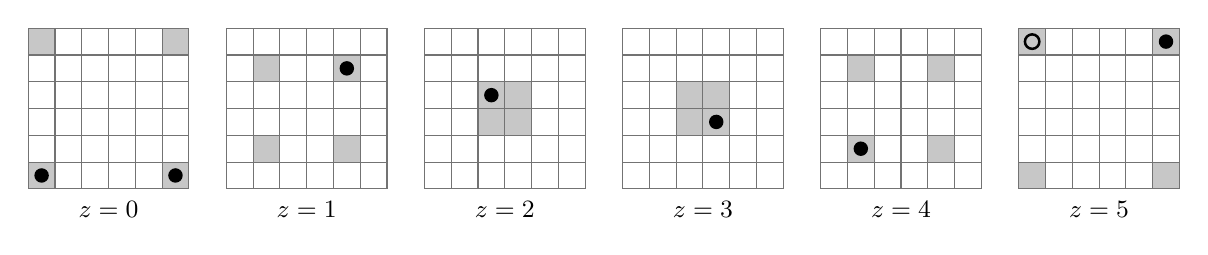
\begin{tikzpicture}[scale=0.34]
\foreach \z in {0,...,5} {
  \begin{scope}[shift={(7.4*\z,0)}]
    \pgfmathtruncatemacro{\w}{5-\z}
    \foreach \x in {\z,\w} { \foreach \y in {\z,\w} { \fill[black!22] (\x,\y) rectangle ++(1,1); } }
    \draw[step=1,black!55,thin] (0,0) grid (6,6);
    \node[below] at (3,-0.1) {\small $z=\z$};
  \end{scope}
}
\foreach \x/\y/\z in {0/0/0,5/0/0,4/4/1,2/3/2,3/2/3,1/1/4,5/5/5}
  { \fill (7.4*\z+\x+0.5,\y+0.5) circle (0.27); }
\draw[line width=0.9pt] (7.4*5+0+0.5,5+0.5) circle (0.27);
\end{tikzpicture}
\caption{The six layers $z=0,\dots,5$ of the board; in each layer $x$ increases to the right and $y$
upwards. Shaded: the $24$ busy cells. Dots: the seven cells of the set $\Tseven$ of \cref{ex:T7};
the set $\Teight$ of \cref{ex:T8} contains in addition the cell $(0,5,5)$ marked by a ring.}
\label{fig:busy}
\end{figure}

\begin{lemma}[Busy cells and lines]\label{lem:busy}
\begin{enumerate}[label=\textup{(\alph*)}]
\item A space diagonal consists of six busy cells, two of each level, and contains the antipode of each
      of its cells. The four space diagonals are pairwise disjoint and partition $\Busy$.
\item Every face diagonal contains exactly two busy cells. An axis line contains two busy cells or none;
      exactly $72$ axis lines contain none, namely those whose two constant coordinates have different
      levels.
\item Two distinct busy cells are collinear if and only if they have the same level or lie on the same
      space diagonal.
\end{enumerate}
\end{lemma}

\begin{proof}
(a) Let $f$ be a parametrization with three active coordinates. The coordinates of $f(t)$ are $t$ or
$5-t$, so $f(t)$ is busy of level $\lambda(t)$, and each level occurs for two values of $t$. For each $i$
we have $5-f_i(t)=f_i(5-t)$, both for $f_i=\mathrm{id}$ and for $f_i=\rho$; hence
$\antip{f(t)}=f(5-t)\in\ell(f)$. By \cref{lem:degree} every busy cell lies on exactly one space diagonal.

(b) On a face diagonal with constant coordinate $v$ the cell with parameter $t$ has the levels
$\lambda(t),\lambda(t),\lambda(v)$ and is busy if and only if $t\in\{v,5-v\}$. On an axis line with constant
coordinates $v,w$ the cell with parameter $t$ is busy if and only if $\lambda(t)=\lambda(v)=\lambda(w)$;
this holds for two values of $t$ if $\lambda(v)=\lambda(w)$ and for none otherwise. For each of the three
directions there are $36-3\cdot 4=24$ pairs $(v,w)$ with $\lambda(v)\ne\lambda(w)$.

(c) Let $p\ne q$ be busy. If both have level $j$, then $(p_i,q_i)\in\{(j,5-j),(5-j,j)\}$ whenever
$p_i\ne q_i$, and $p,q$ are collinear by \cref{cor:collinear} with $(t_1,t_2)=(j,5-j)$. If their levels are
different, then $p_i\ne q_i$ for every $i$, so by \cref{cor:collinear} a line through $p$ and $q$ is a
space diagonal.
\end{proof}

\subsection{Symmetries}\label{ssec:group}

Let $H$ be the group of all permutations $s$ of $\{0,\dots,5\}$ that commute with $\rho$, that is,
$s(5-i)=5-s(i)$ for all $i$. Such an $s$ permutes the three pairs $\{0,5\}$, $\{1,4\}$, $\{2,3\}$ and is
determined by $s(0),s(1),s(2)$, for which there are $6$, $4$ and $2$ possibilities; hence $|H|=48$. We
consider three kinds of maps $\Q\to\Q$:
\begin{itemize}
\item for a permutation $\pi$ of $\{1,2,3\}$, the map $\Pi_\pi$ that moves the $i$-th coordinate to
      position $\pi(i)$: $(\Pi_\pi c)_{\pi(i)}=c_i$;
\item for a set $r\subseteq\{1,2,3\}$, the map $\mathrm{P}_r$ that replaces $c_i$ by $5-c_i$ for every
      $i\in r$;
\item for $s\in H$, the map $\Sigma_s$ that applies $s$ to every coordinate:
      $\Sigma_s(c)=(s(c_1),s(c_2),s(c_3))$.
\end{itemize}
Let
\[
  \G=\{\Sigma_s\circ\mathrm{P}_r\circ\Pi_\pi : s\in H,\ r\subseteq\{1,2,3\},\ \pi\in S_3\}.
\]
The $48$ maps $\mathrm{P}_r\circ\Pi_\pi$ are the symmetries of the cube. The maps $\Sigma_s$ with
$s\notin\{\mathrm{id},\rho\}$ are not isometries: they permute and reverse the three pairs of layers
$\{i,5-i\}$ in all three directions simultaneously. For a map $g$ and a set $Y$ of cells we write
$gY=\{g(c):c\in Y\}$, and $gS=\{gl : l\in S\}$ for a set $S$ of lines.

\begin{lemma}[The group $\G$]\label{lem:group}
\begin{enumerate}[label=\textup{(\alph*)}]
\item Every $g\in\G$ is a bijection of $\Q$ that maps every line onto a line of the same kind (axis line,
      face diagonal, space diagonal). Hence $g$ induces a permutation $l\mapsto gl$ of $\Lines$.
\item $\G$ is closed under composition and under inversion, that is, $\G$ is a group.
\item $|\G|=1{,}152$.
\item Every $g\in\G$ maps $\Busy$ onto $\Busy$ and commutes with the antipodal map:
      $g(\antip{c})=\antip{g(c)}$ for every cell $c$.
\end{enumerate}
\end{lemma}

\begin{proof}
(a) The maps $\Pi_\pi$, $\mathrm{P}_r$, $\Sigma_s$ are bijections with inverses $\Pi_{\pi^{-1}}$,
$\mathrm{P}_r$, $\Sigma_{s^{-1}}$. Let $f$ be a parametrization. Then $\Pi_\pi(\ell(f))=\ell(f')$, where
$f'$ arises from $f$ by permuting the components. Next, $\mathrm{P}_r(\ell(f))=\ell(f')$ with
$f'_i=\rho\circ f_i$ for $i\in r$ and $f'_i=f_i$ otherwise; here $\rho\circ f_i$ is constant, $\rho$ or the
identity if $f_i$ is constant, the identity or $\rho$, respectively. Finally,
$\Sigma_s(\ell(f))=\{(s f_1(t),s f_2(t),s f_3(t)):0\le t\le 5\}$. With the new parameter $t'=s(t)$, which
runs through $\{0,\dots,5\}$ as $t$ does, we have $s(f_i(t))=s(v)$ if $f_i$ is the constant $v$,
$s(f_i(t))=t'$ if $f_i=\mathrm{id}$, and $s(f_i(t))=s(5-t)=5-t'$ if $f_i=\rho$; so
$\Sigma_s(\ell(f))=\ell(f')$, where $f'$ has the same components as $f$ except that each constant $v$ is
replaced by $s(v)$. In all three cases $f'$ is a parametrization with as many active coordinates as $f$.
Thus each of the three kinds of maps, and therefore each $g\in\G$, maps lines onto lines of the same kind.
Being injective on cells, $g$ induces an injective map of the finite set $\Lines$ into itself, that is, a
permutation.

(b) Each of the sets $\G_\Sigma=\{\Sigma_s\}$, $\G_{\mathrm P}=\{\mathrm{P}_r\}$, $\G_\Pi=\{\Pi_\pi\}$ is a
subgroup of the symmetric group of $\Q$, because $\Sigma_s\Sigma_{s'}=\Sigma_{ss'}$,
$\mathrm{P}_r\mathrm{P}_{r'}=\mathrm{P}_{r\triangle r'}$ and $\Pi_\pi\Pi_{\pi'}=\Pi_{\pi\pi'}$. Moreover
\[
  \Sigma_s\Pi_\pi=\Pi_\pi\Sigma_s,\qquad \Sigma_s\mathrm{P}_r=\mathrm{P}_r\Sigma_s,\qquad
  \Pi_\pi\mathrm{P}_r\Pi_\pi^{-1}=\mathrm{P}_{\pi(r)}:
\]
the first relation is obvious, the second holds because $s\rho=\rho s$, and the third says that reversing
the coordinates in $r$ and then moving coordinate $i$ to position $\pi(i)$ is the same as first moving
the coordinates and then reversing those in $\pi(r)$. By the third relation
$K=\G_{\mathrm P}\G_\Pi=\G_\Pi\G_{\mathrm P}$ is a subgroup; by the first two, every element of $\G_\Sigma$
commutes with every element of $K$. Hence $\G=\G_\Sigma K=K\G_\Sigma$ is closed under composition,
$(\sigma\kappa)(\sigma'\kappa')=(\sigma\sigma')(\kappa\kappa')$, and under inversion,
$(\sigma\kappa)^{-1}=\sigma^{-1}\kappa^{-1}$ for $\sigma,\sigma'\in\G_\Sigma$ and $\kappa,\kappa'\in K$.

(c) We have $|\G_\Sigma|=48$. A map $\Pi_\pi$ fixes the cell $(0,0,0)$, while $\mathrm{P}_r(0,0,0)$ has the
entry $5$ exactly in the positions of $r$; hence $\G_{\mathrm P}\cap\G_\Pi=\{\mathrm{id}\}$ and
$|K|=8\cdot 6=48$. Suppose that $\Sigma_s=\mathrm{P}_r\Pi_\pi$, and evaluate both sides at the cells
$(i,i,i)$: the left side is $(s(i),s(i),s(i))$, and the right side has the entry $5-i$ in the positions of
$r$ and the entry $i$ elsewhere. As $i\ne 5-i$, either $r=\emptyset$ and $s=\mathrm{id}$, or $r=\{1,2,3\}$
and $s=\rho$; in both cases $\Sigma_s=\mathrm{P}_r$, so $\Pi_\pi=\mathrm{id}$. Hence
$\G_\Sigma\cap K=\{\mathrm{id},\Sigma_\rho\}$, where $\Sigma_\rho=\mathrm{P}_{\{1,2,3\}}$, and
$|\G|=|\G_\Sigma|\,|K|/|\G_\Sigma\cap K|=48\cdot 48/2=1{,}152$.

(d) By (a), $g$ permutes the space diagonals, and $\Busy$ is their union (\cref{lem:busy}\,(a)). The
antipodal map is $\Sigma_\rho=\mathrm{P}_{\{1,2,3\}}$. It commutes with every $\Sigma_s$ and every
$\mathrm{P}_r$, and with every $\Pi_\pi$ by the third relation above with $r=\{1,2,3\}$.
\end{proof}

The triples $(s,r,\pi)$ thus describe each map of $\G$ exactly twice. The group property in (b) is what
makes canonical forms well behaved (\cref{lem:canon} below).

\subsection{Stones and live lines}\label{ssec:live}

Throughout the paper $B$ denotes a set of cells occupied by \Breaker{} and $X$ a set of cells occupied by
\Maker{} (their \emph{stones}), with $B\cap X=\emptyset$. For a set $Y$ of cells and a cell $c$ we write
$Y+c$ for $Y\cup\{c\}$. A line is \emph{live} (with respect to $B$) if it contains no cell of $B$, and
\emph{dead} otherwise; only live lines can still be completed by \Maker. We write
\[
  \live{B}=\{l\in\Lines : l\cap B=\emptyset\},\qquad \N(S)=\bigcup_{l\in S}l\quad(S\subseteq\Lines)
\]
for the set of live lines and for the set of cells covered by a set $S$ of lines. If $S\subseteq\live{B}$,
then $\N(S)\cap B=\emptyset$. For $g\in\G$ it follows from \cref{lem:group}\,(a) that
\begin{equation}\label{eq:inv-basic}
  \live{gB}=g\,\live{B},\qquad \N(gS)=g\,\N(S),\qquad |gl\cap gY|=|l\cap Y|
\end{equation}
for all sets $B,Y$ of cells, all lines $l$ and all sets $S$ of lines. All notions introduced in
\cref{sec:pairing,sec:leaf} are defined in terms of cells, lines, membership and cardinalities only, and
are therefore invariant under $\G$; the precise statement is \cref{lem:invariance} at the end of
\cref{sec:leaf}.

\subsection{Canonical forms}\label{ssec:canon}

The strategy constructed in this paper is stored as a table of positions, and positions that differ by a
map of $\G$ are stored only once. To this end we order the cells lexicographically, $(x,y,z)<(x',y',z')$
if $x<x'$, or $x=x'$ and $y<y'$, or $x=x'$, $y=y'$ and $z<z'$; equivalently, by the number $36x+6y+z$,
which serves as the name of the cell in the files of \cref{sec:formats}. For two different sets $A,A'$ of
cells we put
\[
  A<A' \quad:\Longleftrightarrow\quad \text{the smallest cell of the symmetric difference }A\triangle A'
  \text{ belongs to }A .
\]
This is a total order on the sets of cells (it is the lexicographic order of the indicator vectors, with
the entry $1$ preceding the entry $0$). For sets of equal size it is the lexicographic order of the
increasingly sorted lists of cells: if $a_1<\dots<a_n$ and $a'_1<\dots<a'_n$ first differ in position $j$
and $a_j<a'_j$, then $a_j$ is the smallest cell of $A\triangle A'$. Pairs of sets are ordered
lexicographically: $(A_1,A_2)<(A'_1,A'_2)$ if $A_1<A'_1$, or $A_1=A'_1$ and $A_2<A'_2$.

\begin{definition}[Canonical form]\label{def:canon}
For two sets $B,F$ of cells, the \emph{canonical form} of the pair $(B,F)$ is
\[
  \canon(B,F)=\min\{(gB,gF) : g\in\G\},
\]
the minimum being taken with respect to the order just defined (the sets $gB$ are compared first). The
pair $(B,F)$ is \emph{canonical} if $\canon(B,F)=(B,F)$.
\end{definition}

In \cref{sec:game} the set $B$ will be the set of \Breaker's stones and $F$ a set of stones of \Maker; a
state of the game there also carries a round number, which is not affected by $\G$.

\begin{lemma}[Canonical forms and translation of moves]\label{lem:canon}
Let $B,F$ be sets of cells.
\begin{enumerate}[label=\textup{(\alph*)}]
\item $\canon(hB,hF)=\canon(B,F)$ for every $h\in\G$.
\item Let $g\in\G$ be any map with $(gB,gF)=\canon(B,F)=:(B^{\mathrm c},F^{\mathrm c})$, let
      $m^{\mathrm c}$ be a cell and $m=g^{-1}(m^{\mathrm c})$. Then $m\notin B\cup F$ if and only if
      $m^{\mathrm c}\notin B^{\mathrm c}\cup F^{\mathrm c}$, and
      \[
        g(B+m)=B^{\mathrm c}+m^{\mathrm c},\qquad g(F+m)=F^{\mathrm c}+m^{\mathrm c};
      \]
      consequently $\canon(B+m,F)=\canon(B^{\mathrm c}+m^{\mathrm c},F^{\mathrm c})$ and
      $\canon(B,F+m)=\canon(B^{\mathrm c},F^{\mathrm c}+m^{\mathrm c})$.
\item If $g,g'\in\G$ both satisfy $(gB,gF)=(g'B,g'F)=\canon(B,F)$, then $h=g'^{-1}g$ satisfies $hB=B$
      and $hF=F$, and $g'^{-1}(m^{\mathrm c})=h\bigl(g^{-1}(m^{\mathrm c})\bigr)$ for every cell
      $m^{\mathrm c}$.
\end{enumerate}
\end{lemma}

\begin{proof}
(a) Since $\G$ is a group (\cref{lem:group}\,(b)), $g\mapsto gh$ is a bijection of $\G$, so the sets
$\{(ghB,ghF):g\in\G\}$ and $\{(gB,gF):g\in\G\}$ coincide. (b) The displayed equations and the equivalence
hold because $g$ is a bijection with $g(m)=m^{\mathrm c}$; the last statement follows from them by (a),
applied to the pairs $(B+m,F)$ and $(B,F+m)$ with $h=g$. (c) is clear, using again that $\G$ is a group.
\end{proof}

Part (b) is the form in which the lemma is used: the table of \cref{sec:game} lists, for a canonical
pair $(B^{\mathrm c},F^{\mathrm c})$, a cell $m^{\mathrm c}$, and in a position described by $(B,F)$ the
move actually played is $m=g^{-1}(m^{\mathrm c})$. Since every property of positions that matters is
invariant under $\G$, the move $m$ is as good in $(B,F)$ as $m^{\mathrm c}$ is in
$(B^{\mathrm c},F^{\mathrm c})$, and the successor positions have the same canonical forms. If the
canonical form is attained by several maps $g$, the resulting moves differ by a symmetry of the pair
$(B,F)$, by (c); the statement (b) holds for each of them and never uses that $g$ is unique. Part (a)
guarantees that it does not matter whether canonical forms are computed from the real position or from a
position that has already been transformed, which is what the different programs of
\cref{sec:verification} do.

\subsection{The full automorphism group}\label{ssec:aut}

An \emph{automorphism} of the board is a bijection of $\Q$ that maps every line onto a line. By
\cref{lem:group} every element of $\G$ is an automorphism. The proof of the main theorem uses nothing
more, but it is natural to ask whether $\G$ misses any symmetry.

\begin{fact}[The full automorphism group; not used in the proof of \cref{thm:main}]\label{fact:aut}
The automorphism group of the incidence structure $(\Q,\Lines)$ has order $1{,}152$; hence it is equal
to~$\G$.

\established the program \fn{autgroup.cpp} in the directory \fn{logs/canon/} of the
project repository (output \fn{autgroup.log}; see \cref{ssec:artifact}), a
search by individualization and color refinement on the incidence graph with $216+148$ vertices. It
finds a base consisting of three lines and three cells; the orbit of each base point under the pointwise
stabilizer of the preceding ones has $4$, $3$, $2$, $6$, $4$, $2$ elements, respectively, so that the
group has order $4\cdot3\cdot2\cdot6\cdot4\cdot2=1{,}152$.
\end{fact}

For the $4\times4\times4$ board the automorphism group, which has order $192$, was determined by
Silver~\cite{Silver1967}, and the automorphism groups of the boards $n^d$ in general were characterized
by Dvo\v{r}\'ak and Valla~\cite{DvorakValla2021}. We did not rely on these results:
\cref{fact:aut} is a direct computation for the present board.

\begin{table}[tb]
\centering\small
\begin{tabular}{@{}lp{0.74\textwidth}@{}}
\toprule
symbol & meaning \\
\midrule
$\Q$, $\Lines$ & the $216$ cells and the $148$ lines (\cref{ssec:lines}) \\
$\lambda(i)$ & level $\min(i,5-i)$ of a coordinate value \\
$\Busy$, $\antip{c}$ & the $24$ busy cells; the antipode of the cell $c$ (\cref{def:busy}) \\
$\G$ & the group of $1{,}152$ symmetries (\cref{lem:group}) \\
$B$, $X$, $F$ & \Breaker's stones, \Maker's stones, the revealed stones of \Maker{} ($F\subseteq X$) \\
$Y+c$ & $Y\cup\{c\}$ \\
$\live{B}$ & the live lines, i.e.\ the lines without a cell of $B$ \\
$\N(S)$ & the union of the lines in $S$ \\
$\canon(B,F)$ & canonical form of a pair of sets (\cref{def:canon}) \\
$\dfc_X(S)$, $\slack(B)$ & deficiency $2|S|-|\N(S)\setminus X|$; slack $216-|B|-2|\live{B}|$ (\cref{sec:pairing}) \\
$\sur_F(S)$, $\Phi(B,F)$ & surplus $|\N(S)\setminus F|-2|S|$; least surplus of an $F$-connected set of
      at least three live lines (\cref{sec:leaf}) \\
$\mu(U)$ & least surplus of a set of live lines containing $U$ (\cref{ssec:deciding}) \\
$\CC$, $\CPhi$, $\LEAF$ & the certificates of \cref{def:C,def:leaf} \\
\bottomrule
\end{tabular}
\caption{Notation introduced in \cref{sec:board,sec:pairing,sec:leaf}.}
\label{tab:notation}
\end{table}
        % 2  The board                         (author A)
\section{Pairings and Hall's condition}\label{sec:pairing}

A pairing strategy is the simplest way in which \Breaker{} can win a game of this kind: he fixes, for
every line, two of its cells, such that the pairs of different lines are disjoint, and whenever \Maker{}
takes a cell of a pair he takes the other one. Pairing strategies for $n^d$ tic-tac-toe go back to
Hales and Jewett~\cite{HalesJewett1963}; see also~\cite{Beck2008,Krivelevich2014}. On the empty $6\times6\times6$ board
there is no pairing, since the $148$ lines would need $296$ cells. In this section we study pairings in
positions in which some lines are already dead and some cells are occupied by \Maker: the strategy that
goes with them (\cref{lem:pairing}), the criterion for their existence (\cref{lem:hall}), and the number
of stones that \Breaker{} needs before a pairing can exist at all.

\subsection{The pairing strategy}\label{ssec:pairing-strategy}

Recall the rules of the Maker--Breaker game on the board: the players alternately occupy an empty cell,
\Maker{} moving first, and \Maker{} wins if at some moment he owns all six cells of a line. A
\emph{position} is described by the disjoint sets $B$ and $X$ of the stones of \Breaker{} and of \Maker;
it is \Maker's turn if $|B|=|X|$, and \Breaker's turn if $|X|=|B|+1$.

\begin{definition}[Pairing]\label{def:pairing}
Let $B,X$ be disjoint sets of cells. A \emph{pairing for $(B,X)$} is a family $\pi=(\pi(l))_{l\in\live{B}}$
of pairwise disjoint sets with $\pi(l)\subseteq l\setminus X$ and $|\pi(l)|=2$ for every live line $l$.
\end{definition}

The cells of $\pi(l)$ are empty: they are not in $X$ by definition and not in $B$ because $l$ is live.
We say that the two cells of $\pi(l)$ are \emph{assigned to} $l$, and that each of them is the
\emph{partner} of the other.

\begin{lemma}[Pairing strategy]\label{lem:pairing}
Consider a position $(B,X)$ with \Maker{} to move, so that $|B|=|X|$, and let $\pi$ be a pairing for
$(B,X)$. Suppose that from now on \Breaker{} answers every move $x$ of \Maker{} by the following rule:
\begin{quote}
if $x\in\pi(l)$ for some $l\in\live{B}$ and the partner of $x$ is empty, take the partner of $x$;
otherwise take an arbitrary empty cell.
\end{quote}
Then, whenever \Breaker{} is to move, the rule names an empty cell, and \Maker{} never owns all six cells
of a line, neither in the position $(B,X)$ nor at any later moment.
\end{lemma}

\begin{proof}
Since $|B|=|X|$ and the players alternate, the number of occupied cells is odd after each move of \Maker,
hence at most $215$: there is an empty cell, and the rule names one. (The line $l$ in the rule is unique,
because the sets $\pi(l)$ are disjoint.)

We claim that the following holds whenever \Maker{} is to move:
\begin{equation}\label{eq:pairing-inv}
  \text{every line $l\in\live{B}$ contains a stone of \Breaker, or both cells of $\pi(l)$ are empty.}
\end{equation}
Here $\live{B}$ refers to the set $B$ of the initial position. In the initial position both cells of
$\pi(l)$ are empty for every $l\in\live{B}$. Assume that \eqref{eq:pairing-inv} holds, let \Maker{} play
$x$ and \Breaker{} reply $z$, and let $l\in\live{B}$. If $l$ contained a stone of \Breaker{} before, it
still does. Otherwise both cells of $\pi(l)$ were empty. If $x\in\pi(l)$, the partner of $x$ is empty, so
$z$ is this partner, and $l$ now contains the stone $z$ of \Breaker. If $x\notin\pi(l)$, then either
$z\in\pi(l)\subseteq l$, and $l$ contains a stone of \Breaker, or both cells of $\pi(l)$ are still empty.
Thus \eqref{eq:pairing-inv} holds again.

Now suppose that at some moment \Maker{} owns all six cells of a line $l$. Then $l$ contains no stone of
\Breaker; in particular $l\cap B=\emptyset$, so $l\in\live{B}$. In the initial position this is
impossible, because $\pi(l)\subseteq l\setminus X$ is not empty. So \Maker{} completed $l$ by a later move
$x$; just before this move he owned five cells of $l$, and $x$ was the only empty cell of $l$. But by
\eqref{eq:pairing-inv}, applied just before the move $x$, the two cells of $\pi(l)\subseteq l$ were both
empty, a contradiction.
\end{proof}

The second alternative of the rule cannot be dispensed with. The partner of $x$ may already hold a stone
of \Breaker, placed earlier as an arbitrary move; the line is then dead, and nothing needs to be done for
it. (The partner of $x$ never holds a stone of \Maker{} when \Maker{} plays $x$: when \Maker{} took the
partner, \Breaker{} answered with $x$ unless $x$ was occupied already.) The
lemma is applied in the proof of \cref{thm:sigma}, from the moment at which \Breaker's strategy switches
from its table to a pairing.

\subsection{Hall's condition}\label{ssec:hall}

Let $B,X$ be disjoint sets of cells. For a set $S\subseteq\live{B}$ of live lines the \emph{deficiency} of
$S$ is
\[
  \dfc_X(S)=2|S|-|\N(S)\setminus X| ,
\]
and we put $\delta(B,X)=\max\{\dfc_X(S):S\subseteq\live{B}\}$; note that $\delta(B,X)\ge\dfc_X(\emptyset)=0$.
An \emph{assignment} for $(B,X)$ is a set of pairs $(l,c)$ with $l\in\live{B}$ and $c\in l\setminus X$ in
which every line occurs at most twice and every cell at most once; a pairing is the same thing as an
assignment with $2|\live{B}|$ pairs. The following lemma is Hall's theorem~\cite{Hall1935} for the
bipartite graph between lines and cells in which every live line is taken twice, in its deficiency
version, together with the usual formulation as a flow
problem~\cite{FordFulkerson1962,Schrijver2003}.

\begin{lemma}[Hall's condition]\label{lem:hall}
Let $B,X$ be disjoint sets of cells and $L=\live{B}$.
\begin{enumerate}[label=\textup{(\alph*)}]
\item The maximum number of pairs in an assignment for $(B,X)$ is $2|L|-\delta(B,X)$.
\item A pairing for $(B,X)$ exists if and only if $\delta(B,X)=0$, that is, if and only if
      \[
         |\N(S)\setminus X|\ge 2|S|\qquad\text{for every } S\subseteq\live{B}.
      \]
\item The number in \textup{(a)} is the value of a maximum flow in the following network $\mathcal N(B,X)$:
      a source $s$, a node for every line $l\in L$, a node for every cell $c\in\N(L)\setminus X$, and a
      sink $t$; arcs $s\to l$ of capacity $2$, arcs $l\to c$ of capacity $1$ for $c\in l\setminus X$, and
      arcs $c\to t$ of capacity $1$.
\item If $X\subseteq X'$ and $X'\cap B=\emptyset$, then $\dfc_X(S)\le\dfc_{X'}(S)$ for every
      $S\subseteq\live{B}$, hence $\delta(B,X)\le\delta(B,X')$; a pairing for $(B,X')$ is also a pairing for
      $(B,X)$.
\item If $B\subseteq B'$ and $B'\cap X=\emptyset$, then the restriction of a pairing for $(B,X)$ to
      $\live{B'}$ is a pairing for $(B',X)$.
\end{enumerate}
\end{lemma}

\begin{proof}
The integral flows in $\mathcal N(B,X)$ are exactly the assignments for $(B,X)$: a flow of $1$ on the arc
$l\to c$ means that the pair $(l,c)$ belongs to the assignment, and the value of the flow is the number of
pairs. As the capacities are integers, there is a maximum flow that is
integral~\cite{FordFulkerson1962}; so the maximum in (a) equals the maximum flow value, and by the
max-flow min-cut theorem it equals the minimum capacity of a cut. Let $A$ be a set of nodes with $s\in A$,
$t\notin A$, and put $S=A\cap L$. The capacity of the cut defined by $A$ is
\[
  2|L\setminus S|+\#\{(l,c): l\in S,\ c\in l\setminus X,\ c\notin A\}+\#\{c : c\in A\}.
\]
Every cell $c\in\N(S)\setminus X$ contributes at least $1$ to the sum of the last two terms: the arc
$c\to t$ if $c\in A$, and an arc $l\to c$ with $l\in S$ otherwise. Hence the capacity is at least
$2|L|-2|S|+|\N(S)\setminus X|=2|L|-\dfc_X(S)$, and equality holds for $A=\{s\}\cup S\cup(\N(S)\setminus X)$.
The minimum capacity of a cut is therefore $2|L|-\delta(B,X)$, which proves (a) and (c). A pairing is an
assignment with $2|L|$ pairs, so (b) is the case $\delta(B,X)=0$ of (a). (d) holds because
$\N(S)\setminus X'\subseteq\N(S)\setminus X$ and $l\setminus X'\subseteq l\setminus X$. (e) holds because
$\live{B'}\subseteq\live{B}$.
\end{proof}

A maximum assignment, and with it either a pairing or a set $S$ violating the condition in (b), is found
by any algorithm for bipartite matching, for instance by augmenting
paths~\cite{FordFulkerson1962,HopcroftKarp1973}. The graphs involved have at most $148$ lines and $216$
cells, and all quantities are small integers; no floating-point arithmetic occurs.

\subsection{Slack, and the number of stones that Breaker needs}\label{ssec:slack}

The simplest obstruction to a pairing is the number of cells.

\begin{definition}[Slack]\label{def:slack}
For a set $B$ of cells, $\slack(B)=(216-|B|)-2\,|\live{B}|$.
\end{definition}

\begin{lemma}\label{lem:slack-bound}
If a pairing for $(B,X)$ exists, then $|X|\le\slack(B)$, and the pairing leaves exactly $\slack(B)-|X|$
cells outside $B\cup X$ unassigned.
\end{lemma}

\begin{proof}
The $2|\live{B}|$ assigned cells are distinct and lie outside $B\cup X$, a set of $216-|B|-|X|$ cells.
\end{proof}

\begin{proposition}[Fewer than seven stones do not suffice]\label{prop:seven}
If $|B|\le 6$, then $\slack(B)<0$, and there is no pairing for $(B,X)$, whatever $X$ is. In particular
there is no pairing on the empty board.
\end{proposition}

\begin{proof}
Every cell lies on at most seven lines (\cref{lem:degree}), so $|\live{B}|\ge 148-7|B|$ and
\[
  \slack(B)\le 216-|B|-2\,(148-7|B|)=13|B|-80\le -2 .
\]
For instance, six stones leave at least $106$ live lines, which need $212$ cells, while only $210$ cells
are free. The claim follows from \cref{lem:slack-bound}.
\end{proof}

So \Breaker{} cannot use a pairing strategy before his seventh move, and when he has made it, \Maker{}
has seven stones on the board as well. For sets of busy cells the slack is easily computed.

\begin{lemma}[Slack of a set of busy cells]\label{lem:busy-slack}
Let $B\subseteq\Busy$ be a set of busy cells that has at most two cells on each of the four space
diagonals, and let $p(B)$ be the number of pairs of collinear cells in $B$; by \cref{lem:busy}\,\textup{(c)}
these are the pairs of cells of $B$ that have the same level or lie on the same space diagonal. Then
\[
  |\live{B}|=148-7|B|+p(B)\qquad\text{and}\qquad \slack(B)=13|B|-80-2p(B).
\]
\end{lemma}

\begin{proof}
A line that is not a space diagonal contains at most two busy cells (\cref{lem:busy}\,(b)); so by the
hypothesis no line contains more than two cells of $B$. Each cell of $B$ lies on seven lines. A dead line
is counted once or twice in the resulting number $7|B|$, and twice if and only if it contains two cells
of $B$. The lines with two cells of $B$ correspond bijectively to the collinear pairs in $B$, because
two cells lie on at most one line (\cref{lem:geometry}\,(c)) and no line contains three cells of $B$.
Hence there are $7|B|-p(B)$ dead lines. The second formula follows from \cref{def:slack}.
\end{proof}

\subsection{Two examples}\label{ssec:examples}

\begin{example}[The set $\Tseven$]\label{ex:T7}
Let
\[
  \Tseven=\{(0,0,0),\ (5,5,5),\ (5,0,0),\ (1,1,4),\ (4,4,1),\ (2,3,2),\ (3,2,3)\}
\]
(see \cref{fig:busy}). All seven cells are busy; the first three have level $0$, the next two level
$1$, the last two level $2$. The cells $(0,0,0),(5,5,5)$ lie on the space diagonal $\{(t,t,t)\}$, the
cells $(1,1,4),(4,4,1)$ on $\{(t,t,5-t)\}$, the cells $(2,3,2),(3,2,3)$ on $\{(t,5-t,t)\}$, and $(5,0,0)$ on
$\{(5-t,t,t)\}$. So no space diagonal contains more than two cells of $\Tseven$, and two cells of
different levels never lie on the same space diagonal. By \cref{lem:busy}\,(c) the collinear pairs are
the pairs of equal level, hence $p(\Tseven)=3+1+1=5$, and by \cref{lem:busy-slack}
\[
  |\live{\Tseven}|=148-49+5=104,\qquad \slack(\Tseven)=209-208=1 :
\]
the seven stones kill $44$ lines, and the $104$ live lines need all but one of the $209$ remaining cells.
\end{example}

\begin{example}[The set $\Teight$]\label{ex:T8}
Let $\Teight=\Tseven+(0,5,5)$. The new cell is busy of level $0$ and lies on the space diagonal
$\{(5-t,t,t)\}$ together with $(5,0,0)$. Again no space diagonal contains more than two cells of
$\Teight$, cells of different levels lie on different space diagonals, and the collinear pairs are the
pairs of equal level: $p(\Teight)=6+1+1=8$. Hence
\[
  |\live{\Teight}|=148-56+8=100,\qquad \slack(\Teight)=208-200=8 :
\]
the eighth stone kills only four further lines (three of the seven lines through it contain one of the
cells $(0,0,0)$, $(5,5,5)$, $(5,0,0)$ and are dead already), but it raises the slack from $1$ to $8$.
\end{example}

\begin{fact}[Pairings for $\Tseven$ and $\Teight$]\label{fact:T-pairings}
There is a pairing for $(\Tseven,\emptyset)$ and a pairing for $(\Teight,\emptyset)$.

\established bipartite matching in the programs \fn{bin/minstones} (for $\Tseven$; output in
\fn{logs/minstones/run.log}), \fn{bin/test_core} (both sets; \fn{logs/core/test_core.log}) and,
with independent code, \fn{bin/treecheck} with the option \fn{--leafcheck}, which reports that $\LEAF(\Tseven,\emptyset,1)$
and $\LEAF(\Teight,\emptyset,8)$ hold (a pairing is part of the predicate $\LEAF$, \cref{def:leaf}), and
in the script \fn{secA_check1.py} in the directory \fn{logs/paper/} of the project repository; the
outputs of the last two are in the file \fn{secA_checks.log} in the same directory (see
\cref{ssec:artifact}).
\end{fact}

Together with \cref{prop:seven} this shows that seven is the least number of stones of \Breaker{} for
which a pairing can exist. A pairing is a certificate that is easy to check, and each of the programs
named above checks the pairing it has found against \cref{def:pairing}.

\subsection{Why this is not yet a strategy}\label{ssec:not-yet}

Neither example gives \Breaker{} a strategy. He needs seven or eight moves to occupy $\Tseven$ or
$\Teight$, and \Maker{} has made as many moves in the meantime. Suppose that after eight rounds
\Breaker{} does own $B=\Teight$, and let $X$ be the set of the eight stones of \Maker. What \Breaker{}
needs is a pairing for $(\Teight,X)$, not for $(\Teight,\emptyset)$, and three things can go wrong.
\begin{itemize}
\item By \cref{lem:slack-bound} a pairing for $(B,X)$ requires $|X|\le\slack(B)$. This rules out
      $\Tseven$, whose slack is $1$, and for $\Teight$ with $|X|=8$ it means that the pairing must use
      \emph{every} remaining cell.
\item Whether a pairing exists depends on where the stones of \Maker{} are. If five of them lie on a live
      line, or if they form two live lines with four stones each that meet in an empty cell, there is no
      pairing (\cref{lem:one-two} below). \Breaker{} can prevent such configurations, but only by
      answering them at once, and such a forced reply is in general not a cell of $\Teight$.
\item \Maker{} may simply occupy cells of $\Teight$ himself.
\end{itemize}
The next section deals with the first two points: it singles out the sets $X$ that \Breaker{} can
enforce by answering immediate threats (the \emph{admissible} sets) and gives a criterion, decidable by
exact integer computations, which guarantees a pairing for $(B,X)$ for every admissible set $X$ that is
compatible with what \Breaker{} knows. For instance, for \emph{every} $\Teight$-admissible set $X$ of
eight cells there is a pairing for $(\Teight,X)$ (\cref{fact:T8-leaf}). The third point,
and the forced replies, are the subject of \cref{sec:game}: there a finite table of moves steers every
play into a position for which the criterion holds.
      % 3  Pairings and Hall's condition     (author A)
\section{Leaf certificates}\label{sec:leaf}

Suppose that after $t$ rounds \Breaker{} wants to switch to a pairing strategy. He knows the set $B$ of his
own stones. The strategy of \cref{sec:game} does not keep track of all stones of \Maker, however, but
only of a subset $F\subseteq X$, the \emph{revealed} stones, and of their total number $t=|X|$. About the
remaining $\theta=t-|F|$ \emph{unrevealed} stones it knows only that $X$ is \emph{admissible}, a condition
that \Breaker{} enforces by answering immediate threats. A \emph{leaf certificate} is a property of the
triple $(B,F,t)$ which guarantees that there is a pairing for $(B,X)$ for \emph{every} set $X$ that is
compatible with this knowledge. In this section we define admissibility (\cref{ssec:adm}), the certificate
$\CC$ that is needed and the stronger certificate $\LEAF$ that is actually computed (\cref{ssec:certs}); we
show how $\LEAF$ is decided by exact integer computations (\cref{ssec:deciding}), prove that it is monotone
in all its arguments (\cref{ssec:monotone}), and examine the case $F=\emptyset$ (\cref{ssec:Fempty}).

\subsection{Admissible sets}\label{ssec:adm}

\begin{definition}[Threats, danger pairs, admissible sets]\label{def:admissible}
Let $B$ and $X$ be disjoint sets of cells; lines are live or dead with respect to $B$.
\begin{itemize}
\item A \emph{threat} of $X$ is a live line with exactly five cells in $X$.
\item A \emph{danger pair} of $X$ is a pair of distinct live lines $a,b$, each with exactly four cells in
      $X$, that have a common cell which is not in $X$. This cell is the \emph{common cell} of the pair; by
      \cref{lem:geometry}\,\textup{(c)} it is the only common cell of $a$ and $b$.
\item $X$ is \emph{$B$-admissible} if every live line has at most four cells in $X$ and $X$ has no danger
      pair.
\end{itemize}
A set $X$ that meets $B$ is not $B$-admissible.
\end{definition}

The two forbidden configurations are the situations in which \Breaker{} has no time to lose. If \Maker{}
has five stones on a live line, \Breaker{} must take its sixth cell at once. If \Maker's stones form a
danger pair $a,b$ with common cell $c$ and \Maker{} is allowed to play $c$, then $a$ and $b$ become
threats simultaneously and only one of them can be answered; the natural reply of \Breaker{} is to take
$c$ himself, which kills both lines. The strategy of \cref{sec:game} makes exactly these replies, and
\cref{lem:threat,lem:danger} show that after such a reply the stones of \Maker{} are admissible again,
unless \Maker{} has created two such configurations by a single move; this requires at least eleven
stones of \Maker{} (\cref{prop:lost-stones}) and does not happen in the positions that matter. In this
way the admissibility of $X$ is an invariant of the first phase of \Breaker's strategy: it holds at the
beginning of every round until \Breaker{} switches to a pairing (\cref{thm:soundness}).
\Cref{lem:one-two} below shows from another side that admissibility is the right hypothesis: it is precisely Hall's
condition for sets of one and two lines, and hence necessary for the existence of a pairing.

\begin{lemma}[Admissibility is inherited]\label{lem:adm-closed}
Let $B$ and $X$ be disjoint sets of cells.
\begin{enumerate}[label=\textup{(\alph*)}]
\item If $X$ is $B$-admissible and $X'\subseteq X$, then $X'$ is $B$-admissible.
\item If $X$ is $B$-admissible, $B\subseteq B'$ and $B'\cap X=\emptyset$, then $X$ is $B'$-admissible.
\item If a set $F$ is not $B$-admissible, then no set $X\supseteq F$ is $B$-admissible.
\end{enumerate}
\end{lemma}

\begin{proof}
(a) Every live line has at most four cells in $X'$. Suppose that $a,b$ is a danger pair of $X'$ with
common cell $c\notin X'$. Then $|a\cap X|\ge 4$ and $|b\cap X|\ge 4$, so both numbers are $4$, because $X$
is admissible; hence $a\cap X=a\cap X'$ and $b\cap X=b\cap X'$. As $c\in a$ and $c\notin X'$, this gives
$c\notin X$. So $a,b$ is a danger pair of $X$, a contradiction. (b) Every line that is live with respect
to $B'$ is live with respect to $B$, and the two conditions of \cref{def:admissible} concern live lines
only. (c) is the contrapositive of (a).
\end{proof}

\begin{lemma}[Admissibility is Hall's condition for one and two lines]\label{lem:one-two}
Let $B$ and $X$ be disjoint sets of cells. Then $X$ is $B$-admissible if and only if
\begin{enumerate}[label=\textup{(\alph*)}]
\item $|l\setminus X|\ge 2$ for every live line $l$, and
\item $|(a\cup b)\setminus X|\ge 4$ for any two distinct live lines $a,b$.
\end{enumerate}
In particular, if there is a pairing for $(B,X)$, then $X$ is $B$-admissible.
\end{lemma}

\begin{proof}
Condition (a) says that every live line has at most four cells in $X$. Assume that this is the case, and
let $a\ne b$ be live lines. If $a\cap b=\emptyset$, then $|(a\cup b)\setminus X|=|a\setminus X|+|b\setminus
X|\ge 4$. Otherwise $a\cap b=\{c\}$ and $|a\cup b|=11$ by \cref{lem:geometry}\,(c). If $c\in X$, then
$|X\cap(a\cup b)|=|X\cap a|+|X\cap b|-1\le 7$, so $|(a\cup b)\setminus X|\ge 4$. If $c\notin X$, then
$|X\cap(a\cup b)|=|X\cap a|+|X\cap b|\le 8$, with equality if and only if both lines have exactly four
cells in $X$, that is, if and only if $a,b$ is a danger pair; so $|(a\cup b)\setminus X|\ge 4$ fails
exactly for danger pairs. Hence, given (a), condition (b) says that there is no danger pair. The last
statement follows from \cref{lem:hall}\,(b), since (a) and (b) are the instances $|S|=1$ and $|S|=2$ of
Hall's condition.
\end{proof}

\subsection{The certificates \texorpdfstring{$\CC$}{C} and \texorpdfstring{$\LEAF$}{LEAF}}\label{ssec:certs}

\begin{definition}[The certificate $\CC$]\label{def:C}
Let $B,F$ be disjoint sets of cells and $k\ge|F|$ an integer. The statement $\CC(B,F,k)$ is:
\begin{quote}
for every $B$-admissible set $X$ with $F\subseteq X$ and $|X|\le k$ there is a pairing for $(B,X)$.
\end{quote}
The number $\theta=k-|F|$ is the number of unrevealed stones that the certificate allows for.
\end{definition}

This is exactly what \Breaker{} needs at the moment described at the beginning of the section, with
$k=t$. We note some immediate properties.

\begin{remark}\label{rem:C}
(i) If $F$ is not $B$-admissible, $\CC(B,F,k)$ holds vacuously, by \cref{lem:adm-closed}\,(c). Such pairs
$(B,F)$ do not occur in a play in which \Maker's stones are admissible; in \cref{sec:game} the
corresponding states are called \VOID.

(ii) $\CC(B,F,k)$ implies $\CC(B,F',k)$ for $F\subseteq F'$, $|F'|\le k$, and $\CC(B,F,k')$ for
$|F|\le k'\le k$, because the sets $X$ in question form a subfamily. The dependence on $B$ is less
obvious; see \cref{prop:leaf-monotone}\,(c) and \cref{sec:extra-monoC}.

(iii) In terms of the deficiency of \cref{lem:hall}, $\CC(B,F,k)$ says that
\[
  \worst(B,F,k)=\max\{\delta(B,X) : X\ B\text{-admissible},\ F\subseteq X,\ |X|\le k\}
\]
is zero (for $B$-admissible $F$; otherwise the maximum is taken over the empty family). This is the
optimum of an integer program, which is described in \cref{sec:ip} and was used as a cross-check only.

(iv) $\CC(B,F,k)$ can be decided by enumeration. By \cref{lem:adm-closed}\,(a) every $B$-admissible set
$X=F\cup\{c_1,\dots,c_m\}$ with $c_1<\dots<c_m$ is reached by adding the cells $c_1,\dots,c_m$ in this
order through admissible sets; so a depth-first enumeration that adds cells in increasing order and
discards inadmissible sets visits every admissible $X\supseteq F$ with $|X|\le k$, and $\CC(B,F,k)$ holds if
and only if there is a pairing at every set visited. It would not be enough to test the sets with
exactly $k$ cells, since an admissible set need not be contained in an admissible set with $k$ cells. The
enumeration is feasible only for small $\theta$; it serves as a further cross-check in
\cref{sec:verification}.
\end{remark}

Since $\CC$ quantifies over all admissible sets $X$, it is expensive to decide. We replace it by a
stronger condition on $(B,F,k)$ in which $X$ no longer occurs.

\begin{definition}[Surplus, adjacency, connected sets of lines]\label{def:surplus}
Let $B$ be a set of cells, $Y$ a set of cells and $S\subseteq\live{B}$.
\begin{itemize}
\item The \emph{surplus} of $S$ is $\sur_Y(S)=|\N(S)\setminus Y|-2|S|=-\dfc_Y(S)$.
\item Two distinct live lines are \emph{$Y$-adjacent} if they have a common cell that is not in $Y$.
\item $S$ is \emph{$Y$-connected} if $S\ne\emptyset$ and the graph with vertex set $S$ whose edges are
      the $Y$-adjacent pairs is connected. The vertex sets of the connected components of this graph are
      the \emph{$Y$-components} of $S$.
\end{itemize}
\end{definition}

We use these notions for $Y=F$ and, in one proof, for $Y=X$. A set $S$ of live lines with
$\sur_F(S)=\sigma\ge 0$ can absorb $\sigma$ further stones of \Maker{} in $\N(S)$ before Hall's condition
fails for $S$; so one would like every set $S$ to have surplus at least $\theta$. For a single line or
for two lines this is too much to ask (their surplus is at most $4$ and $8$), and it is not needed,
because there admissibility takes over (\cref{lem:one-two}). Sets that are not connected need not be
considered either, because the surplus is additive over components (\cref{lem:additive}). This leads to
the following definition.

\begin{definition}[The certificates $\CPhi$ and $\LEAF$]\label{def:leaf}
Let $B,F$ be disjoint sets of cells. Put
\[
  \Phi(B,F)=\min\{\sur_F(S) : S\subseteq\live{B},\ S\ F\text{-connected},\ |S|\ge 3\},
\]
with $\Phi(B,F)=\infty$ if there is no such $S$. For an integer $k\ge|F|$,
\begin{itemize}
\item $\CPhi(B,F,k)$ is the statement $\Phi(B,F)\ge k-|F|$: every $F$-connected set $S$ of at least three
      live lines has $\sur_F(S)\ge k-|F|$;
\item $\LEAF(B,F,k)$ is the conjunction of
  \begin{enumerate}[label=\textup{(L\arabic*)}]
  \item $F$ is $B$-admissible,
  \item there is a pairing for $(B,F)$,
  \item $\CPhi(B,F,k)$.
  \end{enumerate}
\end{itemize}
\end{definition}

\begin{lemma}[Additivity over components]\label{lem:additive}
Let $Y$ be a set of cells, $S\subseteq\live{B}$, and let $S_1,\dots,S_r$ be the $Y$-components of $S$. Then
the sets $\N(S_i)\setminus Y$ are pairwise disjoint. Consequently
\[
  \sur_Y(S)=\sum_{i=1}^r\sur_Y(S_i)\qquad\text{and}\qquad \dfc_Y(S)=\sum_{i=1}^r\dfc_Y(S_i).
\]
\end{lemma}

\begin{proof}
A cell $c\notin Y$ in $\N(S_i)\cap\N(S_j)$, $i\ne j$, would lie on a line of $S_i$ and on a line of $S_j$;
these two lines would be $Y$-adjacent, which is impossible for lines in different components. Hence
$|\N(S)\setminus Y|=\sum_i|\N(S_i)\setminus Y|$, and $|S|=\sum_i|S_i|$.
\end{proof}

\begin{theorem}[$\LEAF$ implies $\CC$]\label{thm:leaf-implies-C}
Let $B,F$ be disjoint sets of cells and $k\ge|F|$. If $\CPhi(B,F,k)$ holds, then $\CC(B,F,k)$ holds. In
particular, $\LEAF(B,F,k)$ implies $\CC(B,F,k)$.
\end{theorem}

\begin{proof}
Let $X$ be a $B$-admissible set with $F\subseteq X$ and $|X|\le k$, and suppose that there is no pairing for
$(B,X)$. By \cref{lem:hall}\,(b) there is a set $S\subseteq\live{B}$ with $\dfc_X(S)>0$. By
\cref{lem:additive}, applied with $Y=X$, some $X$-component $S'$ of $S$ has $\dfc_X(S')>0$, that is,
\begin{equation}\label{eq:violator}
  |\N(S')\setminus X|<2|S'| ,
\end{equation}
and $S'$ is $X$-connected. We distinguish three cases.

\emph{$|S'|=1$.} Then \eqref{eq:violator} contradicts \cref{lem:one-two}\,(a).

\emph{$|S'|=2$.} Then \eqref{eq:violator} contradicts \cref{lem:one-two}\,(b).

\emph{$|S'|\ge 3$.} Since $F\subseteq X$, a common cell of two lines that is not in $X$ is not in $F$; so
$X$-adjacent lines are $F$-adjacent, and $S'$ is $F$-connected. By $\CPhi(B,F,k)$,
\[
  |\N(S')\setminus F|-2|S'|\ \ge\ k-|F|\ \ge\ |X|-|F|\ =\ |X\setminus F|\ \ge\ |(X\setminus F)\cap\N(S')| .
\]
Hence $|\N(S')\setminus X|=|\N(S')\setminus F|-|(X\setminus F)\cap\N(S')|\ge 2|S'|$, contradicting
\eqref{eq:violator}.
\end{proof}

\begin{remark}\label{rem:leaf}
(i) The proof uses only condition (L3). If (L1) fails, $\CC(B,F,k)$ is vacuous (\cref{rem:C}\,(i)).

(ii) Conditions (L1) and (L3) imply (L2): by the theorem $\CC(B,F,k)$ holds, and $X=F$ is a $B$-admissible
set with $|X|\le k$. We keep (L2) in the definition because the algorithm that decides (L3) starts from a
pairing for $(B,F)$; the three conditions are evaluated in this order (\cref{alg:leaf}).

(iii) For $\theta=0$ the certificate is exact. Indeed, $\CPhi(B,F,|F|)$ says that $\sur_F(S)\ge 0$ for
certain sets $S$, which follows from (L2) by \cref{lem:hall}\,(b). So $\LEAF(B,F,|F|)$ holds if and only if
$F$ is $B$-admissible and there is a pairing for $(B,F)$; for $B$-admissible $F$ this is precisely
$\CC(B,F,|F|)$, in which $X=F$ is the only set to be considered.

(iv) In general $\LEAF$ is only sufficient for $\CC$: a set $S$ with small surplus is harmless if the
cells of $\N(S)$ cannot take $\theta$ further stones in an admissible way. \Cref{ex:C-not-leaf} gives an
instance that can be checked by hand; instances with $F\ne\emptyset$ that are closer to positions of the
game were found in the cross-checks of \cref{sec:verification}. The two certificates agree for $\theta=0$
by (iii), and for $F=\emptyset$ and $k\le 10$ by \cref{prop:leaf-equals-C}.
\end{remark}

\begin{example}[$\CC$ holds, $\LEAF$ fails]\label{ex:C-not-leaf}
Let $o=(0,0,0)$, and let $T$ consist of the three lines through $o$ in the plane $x=0$,
\[
  a_1=\{(0,0,t)\},\qquad a_2=\{(0,t,0)\},\qquad a_3=\{(0,t,t)\}\qquad(0\le t\le 5),
\]
so that $|\N(T)|=3\cdot 5+1=16$. Let $B=\Q\setminus\N(T)$, a set of $200$ cells, $F=\emptyset$ and $k=11$.
(This is an instance of the predicates, not a position of the game.)

\emph{$\LEAF(B,\emptyset,11)$ is false.} A line $l\notin T$ meets each line of $T$ in at most one cell, so
it has at most three cells in $\N(T)$ and contains a cell of $B$. Hence $\live{B}=T$. The set $T$ is
$\emptyset$-connected, since its lines have the common cell $o$, and $\sur_\emptyset(T)=16-6=10<11$. So
(L3) fails.

\emph{$\CC(B,\emptyset,11)$ is true.} Let $X$ be $B$-admissible; then $X\subseteq\N(T)$. We claim that
$|X|\le 10$. If $o\in X$, the three numbers $|X\cap a_i|$ are at most $4$ and add up to $|X|+2$. If
$o\notin X$, at most one line of $T$ has four cells in $X$, since two such lines would be a danger pair
with common cell $o$; so $|X|\le 4+3+3$. Now we verify Hall's condition for the non-empty subsets $S$ of
$\live{B}=T$. For $|S|=1$ and $|S|=2$ it holds by \cref{lem:one-two}. For $S=T$ we have
$|\N(T)\setminus X|\ge 16-10=6=2|T|$. By \cref{lem:hall}\,(b) there is a pairing for $(B,X)$.
\end{example}

\subsection{Deciding \texorpdfstring{$\LEAF$}{LEAF}: triples and augmenting paths}\label{ssec:deciding}

Conditions (L1) and (L2) are decided directly from the definitions, (L2) by bipartite matching
(\cref{lem:hall}). Condition (L3) quantifies over all $F$-connected sets of live lines, of which there
may be exponentially many. We show that it suffices to consider the $F$-connected sets of three lines,
and that for each of them the relevant minimum of the surplus is obtained by augmenting a pairing. The
results of this subsection justify the algorithm of \cref{sec:verification} (\cref{alg:leaf}); they are
not needed for the implication $\LEAF\Rightarrow\CC$.

Throughout this subsection $B$ and $F$ are fixed disjoint sets of cells, and $\theta\ge 0$ is an integer.
An \emph{$F$-connected triple} is an $F$-connected set of three live lines. For a set $U\subseteq\live{B}$
let
\[
  \mu(U)=\min\{\sur_F(S) : U\subseteq S\subseteq\live{B}\}.
\]

\begin{lemma}\label{lem:triple}
Every $F$-connected set $S$ of at least three live lines contains an $F$-connected triple.
\end{lemma}

\begin{proof}
A spanning tree of the graph of $F$-adjacency on $S$ has at least three vertices and therefore a vertex
of degree at least $2$ (a tree in which all degrees are at most $1$ has at most one edge). This vertex
and two of its neighbors form an $F$-connected triple.
\end{proof}

\begin{proposition}[Reduction to triples]\label{prop:triples}
Assume that there is a pairing for $(B,F)$.
\begin{enumerate}[label=\textup{(\alph*)}]
\item For every $F$-connected set $U\subseteq\live{B}$ the minimum defining $\mu(U)$ is attained by an
      $F$-connected set:
      \[ \mu(U)=\min\{\sur_F(S) : U\subseteq S\subseteq\live{B},\ S\ F\text{-connected}\}. \]
\item $\Phi(B,F)=\min\{\mu(T) : T \text{ an $F$-connected triple}\}$. Hence $\CPhi(B,F,k)$ holds if and only
      if $\mu(T)\ge k-|F|$ for every $F$-connected triple $T$.
\end{enumerate}
The inequality $\Phi(B,F)\ge\min_T\mu(T)$, and with it the implication ``if'' in \textup{(b)}, holds also
without the assumption.
\end{proposition}

\begin{proof}
(a) The inequality ``$\le$'' is trivial. Let $S\supseteq U$ be an arbitrary subset of $\live{B}$, and let
$S_0$ be the $F$-component of $S$ that contains $U$; it exists because $U$ is $F$-connected. By
\cref{lem:additive}, $\sur_F(S)$ is the sum of $\sur_F(S_0)$ and of the surpluses of the other
$F$-components of $S$, each of which is non-negative by \cref{lem:hall}\,(b), because there is a pairing
for $(B,F)$. Hence $\sur_F(S)\ge\sur_F(S_0)$, where $S_0\supseteq U$ is $F$-connected.

(b) An $F$-connected set $S$ with $|S|\ge 3$ contains an $F$-connected triple $T$ (\cref{lem:triple}), and
$\sur_F(S)\ge\mu(T)$ by the definition of $\mu$; this shows $\Phi(B,F)\ge\min_T\mu(T)$ and does not use the
pairing. Conversely, for an $F$-connected triple $T$ there is by (a) an $F$-connected set $S_0\supseteq T$
with $\sur_F(S_0)=\mu(T)$; as $|S_0|\ge 3$, we get $\Phi(B,F)\le\mu(T)$.
\end{proof}

To compute $\mu(U)$ we let the lines of $U$ collect as many cells as possible, while every other live
line keeps two.

\begin{definition}[$U$-assignments and augmenting paths]\label{def:U-assignment}
Let $U\subseteq\live{B}$.
\begin{itemize}
\item A \emph{$U$-assignment} is a map $\alpha$ from a set $\operatorname{dom}(\alpha)$ of cells to
      $\live{B}$ such that $c\in\alpha(c)$ and $c\notin F$ for every $c\in\operatorname{dom}(\alpha)$, every
      line of $\live{B}\setminus U$ is the image of exactly two cells, and every line of $U$ is the image
      of at least two cells. The cells of $\operatorname{dom}(\alpha)$ are \emph{assigned}; the line $l$
      \emph{holds} the cells of $\alpha^{-1}(l)\subseteq l\setminus F$. The \emph{excess} of $\alpha$ is
      \[
        e(\alpha)=|\operatorname{dom}(\alpha)|-2|\live{B}|=\sum_{l\in U}\bigl(|\alpha^{-1}(l)|-2\bigr).
      \]
\item An \emph{alternating path} from a line $l_0$ (with respect to $\alpha$) is a sequence
      \[ l_0,\,c_1,\,l_1,\,\dots,\,c_j,\,l_j\qquad(j\ge 0) \]
      of distinct live lines $l_i$ and of cells $c_i$ such that
      $c_i\in l_{i-1}\setminus F$ and $\alpha(c_i)=l_i$ for $1\le i\le j$. A line is \emph{reachable} from
      $l_0$ if it is the last line of an alternating path from $l_0$; for a set $U'$ of lines,
      $R_\alpha(U')$ denotes the set of lines that are reachable from some line of $U'$. In particular
      $U'\subseteq R_\alpha(U')$.
\item An \emph{augmenting path} from $l_0$ is an alternating path $l_0,c_1,\dots,l_j$ from $l_0$ together
      with a cell $c_{j+1}\in l_j\setminus F$ that is not assigned. To \emph{augment} $\alpha$ along it
      means to replace $\alpha$ by the map $\alpha'$ with $\alpha'(c_i)=l_{i-1}$ for $1\le i\le j+1$ and
      $\alpha'(c)=\alpha(c)$ for all other $c\in\operatorname{dom}(\alpha)$.
\item A set $R\subseteq\live{B}$ is \emph{closed} (with respect to $\alpha$) if every cell of
      $\N(R)\setminus F$ is held by a line of $R$.
\end{itemize}
\end{definition}

A pairing $\pi$ for $(B,F)$, regarded as the map that sends the two cells of $\pi(l)$ to $l$, is a
$U$-assignment of excess $0$ for every $U$. We record three simple facts about these notions.
\begin{enumerate}[label=\textup{(\roman*)}]
\item In an alternating path the cell $c_i$ is held by $l_i\ne l_{i-1}$, so it is not held by $l_{i-1}$;
      and the cells $c_1,\dots,c_j$ are distinct, because they are held by distinct lines.
\item If $\alpha$ is a $U$-assignment and $l_0\in U$, augmenting along an augmenting path from $l_0$ gives a
      $U$-assignment $\alpha'$ with $e(\alpha')=e(\alpha)+1$. Indeed, the line $l_0$ gains the cell $c_1$;
      each line $l_i$, $1\le i\le j$, loses $c_i$ and gains $c_{i+1}$, which it did not hold; no other line
      is affected; and exactly one new cell, $c_{j+1}$, is assigned.
\item If a line $l$ is reachable from $l_0$, and a cell $c\in l\setminus F$ is held by a line $l'\ne l$,
      then $l'$ is reachable from $l_0$: either $l'$ already occurs on an alternating path from $l_0$ to
      $l$, or this path can be extended by $c,l'$.
\end{enumerate}

\begin{proposition}[Computing $\mu$ by augmentation]\label{prop:maxflow}
Let $\pi$ be a pairing for $(B,F)$ and $U\subseteq\live{B}$.
\begin{enumerate}[label=\textup{(\alph*)}]
\item \textup{(Upper bound.)} For every $U$-assignment $\alpha$ and every set $S$ with
      $U\subseteq S\subseteq\live{B}$ we have $e(\alpha)\le\sur_F(S)$. Hence $e(\alpha)\le\mu(U)$.
\item \textup{(Closed sets persist.)} Let $R$ be closed with respect to a $U$-assignment $\alpha$. Then no
      augmenting path contains a line of $R$. Augmenting $\alpha$ along any augmenting path changes
      $\alpha(c)$ for no cell $c\in\N(R)\setminus F$, and $R$ is closed with respect to the new assignment.
\item \textup{(Witness.)} Let $\alpha$ be a $U$-assignment and $U'\subseteq U$ a set such that there is no
      augmenting path from any line of $U'$. Then $R=R_\alpha(U')$ is closed. If $U'=U$, then moreover
      \[
        \sur_F(R)=e(\alpha)=\mu(U),
      \]
      and $R$ is $F$-connected if $U$ is.
\item \textup{(Augmentation.)} Start with $\alpha=\pi$ and augment repeatedly along augmenting paths from
      lines of $U$, chosen arbitrarily, until there is no such path. Then exactly $\mu(U)$ augmentations
      are performed. In particular, $\mu(U)\ge\theta$ if and only if $\theta$ successive augmentations
      are possible.
\item \textup{(One line at a time.)} Let $U=\{u_1,\dots,u_m\}$. Start with $\alpha=\pi$; augment along
      augmenting paths from $u_1$ until there is none, then along augmenting paths from $u_2$ until there
      is none, and so on. After the step for $u_m$ there is no augmenting path from any line of $U$, so
      that again exactly $\mu(U)$ augmentations have been performed.
\end{enumerate}
\end{proposition}

\begin{proof}
(a) The cells held by the lines of $S$ are distinct cells of $\N(S)\setminus F$. Their number is
$\sum_{l\in S}|\alpha^{-1}(l)|=2|S|+e(\alpha)$, because $U\subseteq S$ and every line outside $U$ holds exactly
two cells. Hence $2|S|+e(\alpha)\le|\N(S)\setminus F|$.

(b) Let $l_0,c_1,\dots,l_j,c_{j+1}$ be an augmenting path and suppose that $l_i\in R$ for some $i\le j$. The
cell $c_{i+1}\in l_i\setminus F$ lies in $\N(R)\setminus F$, so it is held by a line of $R$. In particular
it is assigned, hence $i<j$, and $l_{i+1}=\alpha(c_{i+1})\in R$. Repeating the argument we arrive at
$l_j\in R$ and conclude that $c_{j+1}$ is assigned, a contradiction. Thus no augmenting path contains a
line of $R$. Augmenting changes the value of $\alpha$ only at the cells $c_1,\dots,c_{j+1}$ of the path. If
one of them, say $c_i$, belonged to $\N(R)\setminus F$, it would be held by a line of $R$; then $i\le j$
and $l_i=\alpha(c_i)\in R$, which we have just excluded. So the cells of $\N(R)\setminus F$ keep their
lines, and $R$ remains closed.

(c) Let $l\in R$ and $c\in l\setminus F$. If $c$ were not assigned, an alternating path from a line of
$U'$ to $l$ together with $c$ would be an augmenting path from a line of $U'$. So $c$ is held by a line
$l'$, and $l'=l$ or $l'$ is reachable by fact~(iii) above; in both cases $l'\in R$. Hence $R$ is closed.
Now let $U'=U$, so that $U\subseteq R$. The lines of $R$ hold cells of $\N(R)\setminus F$ only, and every
cell of $\N(R)\setminus F$ is held by a line of $R$; therefore
\[
  |\N(R)\setminus F|=\sum_{l\in R}|\alpha^{-1}(l)|=2|R|+e(\alpha),
\]
again because $U\subseteq R$ and the lines outside $U$ hold exactly two cells. Thus $\sur_F(R)=e(\alpha)$,
and by (a) we get $e(\alpha)\le\mu(U)\le\sur_F(R)=e(\alpha)$. Finally, consecutive lines $l_{i-1},l_i$ of an
alternating path are $F$-adjacent, since they share the cell $c_i\notin F$, and all lines of an
alternating path from a line of $U$ belong to $R$. So every line of $R$ is joined to a line of $U$ by a
path of $F$-adjacent lines inside $R$, and $R$ is $F$-connected if $U$ is.

(d) By fact~(ii) every augmentation yields a $U$-assignment and raises the excess by $1$; by (a) the
excess never exceeds $\mu(U)$, which is finite (take $S=\live{B}$), so the procedure stops. When it stops,
there is no augmenting path from any line of $U$, and $e(\alpha)=\mu(U)$ by (c) with $U'=U$. Since the
excess of $\pi$ is $0$, exactly $\mu(U)$ augmentations were performed. If $\mu(U)\ge\theta$, the procedure
therefore does not stop before the $\theta$-th augmentation; conversely, after $\theta$ augmentations
the excess is $\theta\le\mu(U)$ by (a).

(e) When the step for $u_i$ ends, there is no augmenting path from $u_i$, so $R_i=R_\alpha(\{u_i\})$ is
closed by (c), applied with $U'=\{u_i\}$, and $u_i\in R_i$. By (b), $R_i$ stays closed during all later
augmentations, and as long as $R_i$ is closed there is no augmenting path from $u_i\in R_i$. Hence at the
end there is no augmenting path from any line of $U$, and the number of augmentations is $\mu(U)$ by (d).
\end{proof}

\begin{remark}[Flows]\label{rem:flow}
In the language of flows, let $\mathcal N_U$ be the network $\mathcal N(B,F)$ of \cref{lem:hall}\,(c) in
which the arcs $s\to l$ with $l\in U$ have unbounded capacity. A $U$-assignment is an integral flow in
$\mathcal N_U$ that saturates the arcs $s\to l$ for $l\notin U$ and sends at least two units through
each arc $s\to l$ with $l\in U$; its value is $2|\live{B}|+e(\alpha)$. The
augmenting paths of \cref{def:U-assignment} are the augmenting paths from $s$ to $t$ in the residual
network (they start with an arc $s\to l_0$, $l_0\in U$, since the other arcs out of $s$ are saturated),
and $R_\alpha(U)$ is the set of lines that can be reached from $s$ in the residual network. Thus
\cref{prop:maxflow} says that the maximum flow value of $\mathcal N_U$ is $2|\live{B}|+\mu(U)$, and that
a maximum flow is reached from $\pi$ by exactly $\mu(U)$ augmentations; this also follows from the
max-flow min-cut theorem~\cite{FordFulkerson1962} by the computation in the proof of \cref{lem:hall}.

One point requires care in an implementation that uses a finite capacity on the arcs $s\to l$, $l\in U$.
At most $|l\setminus F|\le 6$ units can pass through a line $l$, so any capacity of at least $6$ gives
the same maximum flow. But with capacity exactly $6$ such an arc is saturated when $l$ holds all its six
cells, and $l$ is then not reachable from $s$ in the residual network: for $U=\{l\}$, $F\cap
l=\emptyset$ and an assignment in which $l$ holds its six cells, no line is reachable from $s$, although
the witness of \cref{prop:maxflow}\,(c) is $R_\alpha(U)\ni l$. To obtain the witness one must either use a
capacity of at least $7$, or add the lines of $U$ to the reachable set explicitly, as
\cref{def:U-assignment} does.
\end{remark}

\begin{corollary}[Pruning rules and quick rejection]\label{cor:pruning}
Let $\pi$ be a pairing for $(B,F)$.
\begin{enumerate}[label=\textup{(\alph*)}]
\item If $U\subseteq U'\subseteq\live{B}$, then $\mu(U)\le\mu(U')$. Hence, for an $F$-connected triple $T$:
      if $\mu(\{l\})\ge\theta$ for one line $l\in T$, or $\mu(\{a,b\})\ge\theta$ for two lines $a,b\in T$,
      then $\mu(T)\ge\theta$.
\item Let $S$ be an $F$-component of the set $\live{B}$ of all live lines. Then the number of cells of
      $\N(S)\setminus F$ that are not assigned by $\pi$ is equal to $\sur_F(S)$. Hence, if $|S|\ge 3$ and
      $\pi$ leaves fewer than $\theta$ cells of $\N(S)\setminus F$ unassigned, then
      $\Phi(B,F)\le\sur_F(S)<\theta$.
\end{enumerate}
\end{corollary}

\begin{proof}
(a) The minimum defining $\mu(U')$ is taken over a subfamily of the sets admitted for $\mu(U)$. (b) Let
$c\in\N(S)\setminus F$ be assigned to a line $l'$, and let $l\in S$ be a line through $c$. If $l'\ne l$,
then $l'$ and $l$ are $F$-adjacent, so $l'\in S$, because $S$ is a component of the whole set $\live{B}$.
Thus every assigned cell of $\N(S)\setminus F$ is held by a line of $S$. Conversely, the $2|S|$ cells held
by the lines of $S$ lie in $\N(S)\setminus F$. So exactly $2|S|$ cells of $\N(S)\setminus F$ are assigned,
and $|\N(S)\setminus F|-2|S|=\sur_F(S)$ are not.
\end{proof}

Since a single line holds at most six cells and two lines at most twelve, we have $\mu(\{l\})\le 4$ and
$\mu(\{a,b\})\le 8$; so the first rule in (a) can apply only for $\theta\le 4$ and the second only for
$\theta\le 8$. In (b), counting the cells of $F\cap\N(S)$ as unassigned as well makes the test weaker but
leaves it valid.

\medskip\noindent\textbf{An exact test for $\LEAF$.}
Together these results give the following procedure for deciding $\LEAF(B,F,k)$, where
$\theta=k-|F|\ge 0$. All its steps are computations with small integers on a bipartite graph with at
most $148+216$ vertices.
\begin{enumerate}[label=\textup{\arabic*.}]
\item Test whether $F$ is $B$-admissible (\cref{def:admissible}). If not, $\LEAF(B,F,k)$ is false.
\item Compute a maximum assignment for $(B,F)$ by augmenting paths (\cref{lem:hall}). If some live line
      receives fewer than two cells, there is no pairing and $\LEAF(B,F,k)$ is false. Otherwise a pairing
      $\pi$ has been found.
\item Optionally, apply the quick rejection of \cref{cor:pruning}\,(b) to the $F$-components of
      $\live{B}$ with at least three lines.
\item For every $F$-connected triple $T$ (a line together with two lines that are $F$-adjacent to it),
      decide whether $\mu(T)\ge\theta$: starting from $\pi$, try to perform $\theta$ augmentations from
      the lines of $T$ (\cref{prop:maxflow}\,(d) or (e)). A triple may be skipped if one of its lines or
      pairs of lines is already known to satisfy $\mu\ge\theta$ (\cref{cor:pruning}\,(a)). If the
      procedure stops after fewer than $\theta$ augmentations, then $R=R_\alpha(T)$ is an $F$-connected
      set of at least three live lines with $\sur_F(R)=\mu(T)<\theta$ (\cref{prop:maxflow}\,(c)), and
      $\LEAF(B,F,k)$ is false.
\item If every triple passes, $\LEAF(B,F,k)$ is true (\cref{prop:triples}\,(b)).
\end{enumerate}
A negative answer in steps 3 and 4 comes with a set $S$ of lines whose surplus can be recomputed from
the definition, and a positive answer for a triple $T$ comes with a $T$-assignment of excess $\theta$,
which by \cref{prop:maxflow}\,(a) proves $\sur_F(S)\ge\theta$ for all $S\supseteq T$ without any reference
to the way in which it was found. For the soundness of the main theorem only positive answers matter,
and for these the argument just given, \cref{lem:triple} and \cref{thm:leaf-implies-C} suffice.

\subsection{Monotonicity}\label{ssec:monotone}

The certificate $\LEAF$ can only improve when more stones of \Maker{} are revealed, when fewer stones
have to be allowed for, and when \Breaker{} has more stones.

\begin{proposition}[Monotonicity of $\LEAF$]\label{prop:leaf-monotone}
Assume that $\LEAF(B,F,k)$ holds.
\begin{enumerate}[label=\textup{(\alph*)}]
\item If $F\subseteq F'$, $F'$ is $B$-admissible and $|F'|\le k$, then $\LEAF(B,F',k)$ holds.
\item If $|F|\le k'\le k$, then $\LEAF(B,F,k')$ holds.
\item If $b$ is a cell with $b\notin F$, then $\LEAF(B+b,F,k)$ holds.
\end{enumerate}
\end{proposition}

\begin{proof}
(a) (L1) is assumed. (L2): by \cref{thm:leaf-implies-C}, $\CC(B,F,k)$ holds, and $F'$ is a $B$-admissible
set with $F\subseteq F'$ and $|F'|\le k$; so there is a pairing for $(B,F')$. (L3): let $S$ be an
$F'$-connected set of at least three live lines. A common cell of two lines outside $F'$ is outside
$F$, so $S$ is $F$-connected, and
\[
  \sur_{F'}(S)=\sur_F(S)-|\N(S)\cap(F'\setminus F)|\ \ge\ (k-|F|)-|F'\setminus F|=k-|F'| .
\]

(b) (L1) and (L2) do not involve $k$, and $k'-|F|\le k-|F|$.

(c) (L1) holds by \cref{lem:adm-closed}\,(b), since $(B+b)\cap F=\emptyset$. (L2) holds by
\cref{lem:hall}\,(e). (L3): a set of lines that are live with respect to $B+b$ is a set of lines that are
live with respect to $B$, and neither $F$-adjacency nor $\sur_F$ depends on $B$.
\end{proof}

In terms of \cref{def:leaf}, (a) says that $\Phi(B,F')\ge\Phi(B,F)-|F'\setminus F|$ and (c) says that
$\Phi(B+b,F)\ge\Phi(B,F)$. These properties make $\LEAF$ well suited to a search for certificates; within
this paper, (a) is used in the proof of \cref{prop:lazy-monotone}, and \cref{thm:soundness} does not
depend on the proposition. For the certificate $\CC$ the analogue of (c) is true only for $B$-admissible
$F$, and its proof is considerably longer; it is given in \cref{sec:extra-monoC} and is not used
anywhere.

\subsection{The case \texorpdfstring{$F=\emptyset$}{F empty}}\label{ssec:Fempty}

For $F=\emptyset$ two lines are adjacent if they meet, and we write $\sur(S)$ for $\sur_\emptyset(S)$ and
``connected'' for ``$\emptyset$-connected''. By \cref{lem:geometry}\,(c) a connected set $T$ of three
lines is of one of three kinds:
\begin{itemize}
\item a \emph{triangle}: the three lines meet pairwise, in three distinct cells; $|\N(T)|=18-3=15$ and
      $\sur(T)=9$;
\item a \emph{star}: the three lines pass through one cell; $|\N(T)|=16$ and $\sur(T)=10$;
\item a \emph{path}: two of the lines are disjoint and the third meets both; $|\N(T)|=16$ and
      $\sur(T)=10$.
\end{itemize}
(If the three lines meet pairwise and two of the three meeting cells coincide, this cell lies on all
three lines, and all three meeting cells coincide.)

\begin{lemma}[Ten admissible stones on three lines]\label{lem:433}
Let $a_1,a_2,a_3$ be three distinct live lines, and call a cell of $a_i$ \emph{private} if it lies on
neither of the other two lines. Then each $a_i$ has at least four private cells. If $X_T$ consists of
four private cells of $a_1$, three private cells of $a_2$ and three private cells of $a_3$, then
$|X_T|=10$, and $X_T$ and all its subsets are $B$-admissible.
\end{lemma}

\begin{proof}
Each $a_i$ meets each of the other two lines in at most one cell, so at least four of its cells are
private. A private cell of $a_j$ does not lie on $a_i$ for $i\ne j$; hence the ten chosen cells are
distinct, and $a_1,a_2,a_3$ contain exactly $4$, $3$, $3$ cells of $X_T$. Any other line meets each $a_i$
in at most one cell and so contains at most three cells of $X_T$. Thus no line has more than four cells
in $X_T$, and only one line has four, so there is no danger pair. Moreover $X_T\cap B=\emptyset$, because
the lines are live. The subsets of $X_T$ are $B$-admissible by \cref{lem:adm-closed}\,(a).
\end{proof}

\begin{proposition}[$\LEAF$ is exact for $F=\emptyset$, $k\le 10$]\label{prop:leaf-equals-C}
For every set $B$ of cells and every integer $k$ with $0\le k\le 10$,
\[
  \CC(B,\emptyset,k)\iff\LEAF(B,\emptyset,k).
\]
\end{proposition}

\begin{proof}
``$\Leftarrow$'' is \cref{thm:leaf-implies-C}. For ``$\Rightarrow$'' assume $\CC(B,\emptyset,k)$. Condition
(L1) is trivial, and (L2) is $\CC(B,\emptyset,k)$ applied to $X=\emptyset$. Suppose that (L3) fails: there is
a connected set $S\subseteq\live{B}$ with $|S|\ge 3$ and $\sur(S)\le k-1\le 9$. By (L2) and
\cref{lem:hall}\,(b), $\sur(S)\ge 0$. Put $j=\sur(S)+1$, so that $1\le j\le k\le 10$. Choose a connected
triple $T\subseteq S$ (\cref{lem:triple}) and a subset $X$ with $j$ elements of a set $X_T$ as in
\cref{lem:433}. Then $X$ is $B$-admissible, $|X|=j\le k$, and $X\subseteq\N(T)\subseteq\N(S)$, so that
\[
  |\N(S)\setminus X|=|\N(S)|-j=2|S|+\sur(S)-j=2|S|-1<2|S| .
\]
By \cref{lem:hall}\,(b) there is no pairing for $(B,X)$, which contradicts $\CC(B,\emptyset,k)$.
\end{proof}

The bound $10$ is the size of $X_T$. For $k\ge 11$, or for $F\ne\emptyset$, the construction is not
available, and $\LEAF$ is only sufficient for $\CC$ (\cref{ex:C-not-leaf}).

\begin{corollary}[Slack is necessary]\label{cor:slack-necessary}
Let $B$ be a set of cells with at least three live lines and let $k\le 10$. If $\LEAF(B,\emptyset,k)$
holds, then $\slack(B)\ge k$.
\end{corollary}

\begin{proof}
Choose three live lines and a subset $X$ with $k$ elements of a set $X_T$ as in \cref{lem:433}. By
\cref{thm:leaf-implies-C} there is a pairing for $(B,X)$, and $k=|X|\le\slack(B)$ by
\cref{lem:slack-bound}.
\end{proof}

For $F=\emptyset$ a triangle of live lines limits the certificate to $k\le 9$, since its surplus is $9$.
Sets of busy cells cannot destroy all triangles unless they are large:

\begin{proposition}[Busy sets with at most eleven cells]\label{prop:busy10}
Let $B\subseteq\Busy$ be a set of busy cells with $|B|\le 11$. Then $\live{B}$ contains a triangle.
Consequently $\Phi(B,\emptyset)\le 9$, and $\LEAF(B,\emptyset,k)$ and $\CC(B,\emptyset,k)$ are false for
every $k\ge 10$. In particular, $\LEAF(B,\emptyset,10)$ is false for every set $B$ of ten busy cells.
\end{proposition}

\begin{proof}
A busy cell lies on exactly three face diagonals (\cref{lem:degree}). So at most $33$ of the $36$ face
diagonals contain a cell of $B$, and there is a live face diagonal $d$. A permutation of the coordinates
maps lines onto lines and busy cells onto busy cells (\cref{lem:group}); we may therefore assume that the
constant coordinate of $d$ is the third one, with value $v$, so that
\[
  d=\{(t,t,v):0\le t\le 5\}\qquad\text{or}\qquad d=\{(t,5-t,v):0\le t\le 5\}.
\]
There are four values in $\{0,\dots,5\}$ whose level is different from $\lambda(v)$, and they form two
pairs $\{i,5-i\}$. Let $r$ be a value from one of these pairs and $s$ a value from the other; thus
$\lambda(r)\ne\lambda(v)$, $\lambda(s)\ne\lambda(v)$, and $s\notin\{r,5-r\}$. Consider the axis lines
\[
  a=\{(t,r,v):0\le t\le 5\}\qquad\text{and}\qquad b=\{(s,t,v):0\le t\le 5\}.
\]
By \cref{lem:busy}\,(b) neither of them contains a busy cell, since their constant coordinates have
different levels. Hence $a$ and $b$ are live, like $d$. We have $a\cap b=\{(s,r,v)\}$, and
\[
  d\cap a=\{(r,r,v)\},\quad d\cap b=\{(s,s,v)\}\qquad\text{or}\qquad
  d\cap a=\{(5-r,r,v)\},\quad d\cap b=\{(s,5-s,v)\}
\]
in the two cases. Since $s\ne r$ and $s\ne 5-r$, the three meeting cells are distinct in both cases. So
$T=\{d,a,b\}$ is a triangle of live lines.

Now $T$ is a connected set of three live lines with $\sur(T)=15-6=9$; hence $\Phi(B,\emptyset)\le 9$, and
$\LEAF(B,\emptyset,k)$ is false for $k\ge 10$. By \cref{prop:leaf-equals-C}, $\CC(B,\emptyset,10)$ is false,
and so is $\CC(B,\emptyset,k)$ for every $k\ge 10$ by \cref{rem:C}\,(ii).
\end{proof}

\begin{figure}[t]
\centering
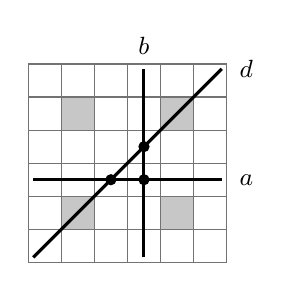
\begin{tikzpicture}[scale=0.42]
\foreach \x in {1,4} { \foreach \y in {1,4} { \fill[black!22] (\x,\y) rectangle ++(1,1); } }
\draw[step=1,black!55,thin] (0,0) grid (6,6);
\draw[line width=1.1pt] (0.15,0.15) -- (5.85,5.85);
\draw[line width=1.1pt] (0.15,2.5) -- (5.85,2.5);
\draw[line width=1.1pt] (3.5,0.15) -- (3.5,5.85);
\fill (2.5,2.5) circle (0.17); \fill (3.5,3.5) circle (0.17); \fill (3.5,2.5) circle (0.17);
\node[right] at (6.1,5.85) {\small $d$};
\node[right] at (6.1,2.5) {\small $a$};
\node[above] at (3.5,6.0) {\small $b$};
\end{tikzpicture}
\caption{The triangle in the proof of \cref{prop:busy10}, drawn in the plane $z=v$ for $v=1$, with
$d=\{(t,t,1)\}$, $r=2$ and $s=3$ ($x$ to the right, $y$ upwards). Shaded: the four busy cells of the
plane. The lines $a$ (row $y=r$) and $b$ (column $x=s$) contain no busy cell.}
\label{fig:triangle}
\end{figure}

More generally, if $T$ is a triangle of live lines none of whose three meeting cells belongs to $F$,
then $T$ is $F$-connected and $\Phi(B,F)\le\sur_F(T)=9-|F\cap\N(T)|$. In the certificate of
\cref{sec:certificate} the largest number of unrevealed stones at a leaf is $\theta=8$.

We finally return to the examples of \cref{ssec:examples}.

\begin{fact}[The sets $\Teight$ and $\Tseven$]\label{fact:T8-leaf}
\begin{enumerate}[label=\textup{(\alph*)}]
\item $\LEAF(\Teight,\emptyset,8)$ holds. Equivalently, by \cref{prop:leaf-equals-C}: for every
      $\Teight$-admissible set $X$ of at most eight cells there is a pairing for $(\Teight,X)$.
\item The set $\live{\Teight}$ of all $100$ live lines is connected and covers the $208$ cells outside
      $\Teight$; so $\sur(\live{\Teight})=208-200=8$, and $\Phi(\Teight,\emptyset)=8$.
\item The set $\live{\Tseven}$ of all $104$ live lines is connected and covers the $209$ cells outside
      $\Tseven$; so $\sur(\live{\Tseven})=1$. Moreover $\LEAF(\Tseven,\emptyset,1)$ holds, and
      $\Phi(\Tseven,\emptyset)=1$.
\end{enumerate}

\established the program \fn{bin/phicheck} (\fn{src/phi.hpp}) and, with independent code, the
program \fn{bin/treecheck} with the option \fn{--leafcheck}. On the four instances
$(\Teight,\emptyset,8)$, $(\Teight,\emptyset,9)$, $(\Tseven,\emptyset,1)$, $(\Tseven,\emptyset,2)$ both
programs report $\LEAF$ to be true, false, true, false, and
for the two negative answers \fn{phicheck} returns the set of all live lines as its witness, with
surplus $8$ and $1$; the outputs are in the file \fn{secA_checks.log} in the directory
\fn{logs/paper/} of the project repository (see \cref{ssec:artifact}). The same values are recorded in
\fn{logs/core/test_core.log} and in the regression file \fn{ip_regression.json} in \fn{results/regression/}. They were confirmed,
together with the statements on connectedness and covering in (b) and (c), by a third program with its
own geometry and its own augmenting-path code (\fn{secA_check1.py} in \fn{logs/paper/}).
\end{fact}

That $\LEAF(\Teight,\emptyset,9)$ and $\LEAF(\Tseven,\emptyset,k)$ for $k\ge 2$ fail does not depend on a
computation: it follows from \cref{cor:slack-necessary}, because $\slack(\Teight)=8$ and
$\slack(\Tseven)=1$ (\cref{ex:T7,ex:T8}). Thus $\Teight$ is a set with which \Breaker{} could switch to a
pairing strategy after eight rounds, provided that \Maker's eight stones are admissible; but there is no
margin, and $\Tseven$ is useless for this purpose. How \Breaker{} reaches a position with a leaf
certificate against every defense of \Maker{} is the subject of the next two sections.

\subsection{Invariance under the symmetry group}\label{ssec:invariance}

For $g\in\G$ and a family $\pi=(\pi(l))_{l\in\live{B}}$ let $g\pi$ denote the family
$(g\pi(g^{-1}l'))_{l'\in\live{gB}}$; recall that $\live{gB}=g\,\live{B}$ by \eqref{eq:inv-basic}.

\begin{lemma}[Invariance]\label{lem:invariance}
Let $g\in\G$, let $B,X,F$ be sets of cells, $S\subseteq\live{B}$, and $k$ an integer.
\begin{enumerate}[label=\textup{(\alph*)}]
\item $\live{gB}=g\,\live{B}$, $\N(gS)=g\,\N(S)$ and $\slack(gB)=\slack(B)$.
\item $X$ is $B$-admissible if and only if $gX$ is $gB$-admissible; the threats and danger pairs of $gX$
      with respect to $gB$ are the images of those of $X$ with respect to $B$.
\item $\pi$ is a pairing for $(B,X)$ if and only if $g\pi$ is a pairing for $(gB,gX)$.
\item $\sur_{gF}(gS)=\sur_F(S)$ and $\dfc_{gX}(gS)=\dfc_X(S)$; two live lines $a,b$ are $F$-adjacent if and
      only if $ga,gb$ are $gF$-adjacent; $S$ is $F$-connected if and only if $gS$ is $gF$-connected; and
      $\Phi(gB,gF)=\Phi(B,F)$.
\item Each of the statements $\CC(B,F,k)$, $\CPhi(B,F,k)$ and $\LEAF(B,F,k)$ holds if and only if the
      corresponding statement holds for $(gB,gF,k)$.
\end{enumerate}
\end{lemma}

\begin{proof}
By \cref{lem:group}, $g$ is a bijection of the cells that induces a bijection $l\mapsto gl$ of the lines,
and $g^{-1}\in\G$. Hence $c\in l$ if and only if $g(c)\in gl$, and $g$ preserves cardinalities,
inclusions, intersections and unions of sets of cells. All notions in (a)--(e) are defined in these
terms: a line $l$ is live for $B$ if and only if $gl$ is live for $gB$; $|gl\cap gX|=|l\cap X|$; a cell
$c$ is a common cell of $a$ and $b$ outside $X$ if and only if $g(c)$ is a common cell of $ga$ and $gb$
outside $gX$; and $|\N(gS)\setminus gY|=|\N(S)\setminus Y|$, $|gS|=|S|$. This gives (a)--(d). For (e), the
map $X\mapsto gX$ is a bijection from the $B$-admissible sets $X\supseteq F$ with $|X|\le k$ onto the
$gB$-admissible sets containing $gF$ with at most $k$ cells, by (b), and it preserves the existence of
a pairing, by (c); the statements for $\CPhi$ and $\LEAF$ follow from (b), (c) and (d).
\end{proof}
         % 4  Leaf certificates                 (author A)
% sec_game.tex -- Section 5: The abstract game and its soundness (author B)

\section{The abstract game and its soundness}\label{sec:game}

On the empty board no pairing exists (the $148$ lines would need $296$ cells), so \Breaker{} cannot follow a
pairing strategy from the first move. Instead \Breaker{} first places stones according to a finite table until
the leaf certificate $\LEAF(B,F,t)$ of \cref{def:leaf} holds, and plays a pairing strategy from then
on. This section makes the table precise. We define a finite \emph{abstract game} whose states are labeled
\WON{} by a recursion, and \emph{certificates}, which are finite witnesses for the statement that the root of
the abstract game is \WON. From a certificate we define a strategy $\sigma$ for \Breaker{} and prove that
$\sigma$ always prescribes an empty cell and never lets \Maker{} own a whole line
(\cref{thm:soundness,thm:sigma}). Together with a strategy-stealing argument this proves
\cref{thm:main}. Every statement of this section is proved by hand. The existence of a certificate
(\cref{fact:H}) enters only as a hypothesis.

\medskip\noindent\textbf{Conventions.}
Throughout, $B$ and $X$ are disjoint sets of cells: the stones of \Breaker{} and of \Maker. Lines are live
with respect to $B$, and $\live{B}$ is the set of live lines. We write $B+e$ for $B\cup\{e\}$. By
\cref{lem:geometry}\,(c) two distinct lines have at most one common cell; this is used constantly, and
references to \cref{lem:geometry} always mean this statement. We use
the terminology of \cref{def:admissible}: a \emph{threat} of $X$ is a live line with exactly five cells in
$X$; a \emph{danger pair} of $X$ consists of two distinct live lines, each with exactly four cells in $X$,
which share a cell outside $X$ (the \emph{common cell} of the pair); and $X$ is \emph{$B$-admissible} if
$X\cap B=\emptyset$, every live line has at most four cells in $X$, and $X$ has no danger pair. Threats and
danger pairs always refer to the set $B$ under consideration, and both words are used for arbitrary sets
$X$ disjoint from $B$, admissible or not. \cref{lem:adm-closed} is used in the following form: if $X$ is
$B$-admissible, then every subset of $X$ is $B$-admissible (part (a)), and $X$ is $B'$-admissible for every
$B'\supseteq B$ that is disjoint from $X$ (part (b)).

\subsection{Lazy revelation}\label{sec:lazy}

A table that lists a reply of \Breaker{} to every position would have to branch, at each move of \Maker, over
all empty cells, of which there are more than $190$ during the first ten rounds. The abstract game avoids
almost all of this branching. It rests on the observation that, as long as \Breaker{} follows a table, the
stones of \Maker{} matter in two ways only.
\begin{enumerate}[label=\textup{(\roman*)},leftmargin=2.2em]
\item \emph{Forced events.} If a move of \Maker{} creates a threat, \Breaker{} must occupy the sixth cell of
  that line at once. If it creates a danger pair, \Breaker{} occupies the common cell of the pair, since
  otherwise \Maker{} could occupy it and create two threats with one move. These are the \emph{forced
  replies}. A forced reply is determined by the stones of \Maker{} on the one or two lines involved, and these
  stones count as \emph{revealed} from then on.
\item \emph{Occupied cells.} If the table tells \Breaker{} to occupy a cell $m$ that already holds a stone of
  \Maker, then this stone is revealed, and \Breaker{} consults the table again.
\end{enumerate}
Accordingly \Breaker{} keeps a \emph{record} $(B,F,t)$: the set $B$ of \Breaker's own stones, the set $F$ of
revealed stones of \Maker, and the number $t$ of completed rounds. The table is indexed by records. The other
$\theta=t-|F|$ stones of \Maker{} are \emph{unrevealed}: \Breaker{} sees them on the board, of course, but
the table does not depend on where they are. A move of \Maker{} that causes no forced event therefore leads
to a single successor record, whichever cell was taken. We call this \emph{lazy revelation}.

Two things have to be paid for. First, at the moment when \Breaker{} stops consulting the table and switches
to a pairing strategy, a pairing must exist for the real position, while the record knows only $F$. As long
as every forced reply has restored admissibility, the set $X$ of \Maker's stones is $B$-admissible at this
moment. So what is needed is a pairing for every $B$-admissible set $X\supseteq F$ with $|X|=t$. This is
guaranteed by the condition $\CC(B,F,t)$ of \cref{def:C}, which by \cref{thm:leaf-implies-C} follows from
the efficiently checkable condition $\LEAF(B,F,t)$. Second, a forced reply need not restore admissibility:
a move of \Maker{} may create a threat together with a danger pair that the forced reply does not destroy,
or two danger pairs that no single reply destroys. Such a move needs at least eleven stones of \Maker{} in
special position (\cref{prop:lost-stones}), and the abstract game excludes it by a conservative
test, $\LOST$, on the record (\cref{def:lost}).

The table itself uses the real position only through the record. The real position enters the strategy
$\sigma$ in three places: the detection of forced events, the test whether the cell named by the table is
occupied, and the pairing computed at the end. Nothing in this section depends on which cells the table
names; in particular they need not be busy cells.

\subsection{States and children}\label{sec:states}

\begin{definition}[States and their children]\label{def:states}\label{def:children}
Let $t\ge 0$ be an integer and let $B,F\subseteq\Q$ be disjoint sets of cells.
\begin{itemize}[leftmargin=2.2em]
\item $\Pst(B,F,t)$ is a \emph{P-state} if $|B|=t$ and $|F|\le t$. (\Maker{} is to move; $t$ rounds have been
  completed.)
\item $\Qst(B,F,t)$ is a \emph{Q-state} if $t\ge 1$, $|B|=t-1$ and $|F|\le t$. (\Breaker{} is to move in round
  $t$, after a move of \Maker{} that caused no forced event.)
\item A state is \VOID{} if $F$ is not $B$-admissible.
\item The \emph{root} is the P-state $\Pst(\emptyset,\emptyset,0)$.
\end{itemize}
In both kinds of states $B$ stands for the stones of \Breaker, $F$ for the revealed stones of \Maker, and
$\theta=t-|F|$ is the number of unrevealed stones of \Maker.

The \emph{children} of a P-state $\Pst(B,F,t)$ are the following states.
\begin{enumerate}[leftmargin=2.6em]
\item[\textup{(a)}] \emph{Quiet move:} the Q-state $\Qst(B,F,t+1)$.
\item[\textup{(c)}] \emph{Threat:} for every live line $l\in\live{B}$ and every cell $e\in l\setminus F$ with
  $|F\cup(l\setminus\{e\})|\le t+1$, the P-state
  \[ \Pst\bigl(B+e,\;F\cup(l\setminus\{e\}),\;t+1\bigr). \]
\item[\textup{(d)}] \emph{Danger:} for every unordered pair of distinct live lines $a,b\in\live{B}$ that meet,
  say $a\cap b=\{c\}$, with $c\notin F$, and for all sets $Q_a\subseteq a\setminus\{c\}$ and
  $Q_b\subseteq b\setminus\{c\}$ with
  \[ |Q_a|=|Q_b|=4,\qquad F\cap a\subseteq Q_a,\qquad F\cap b\subseteq Q_b,\qquad |F\cup Q_a\cup Q_b|\le t+1, \]
  the P-state
  \[ \Pst\bigl(B+c,\;F\cup Q_a\cup Q_b,\;t+1\bigr). \]
\end{enumerate}
The \emph{children} of a Q-state $\Qst(B,F,t)$ \emph{via} a cell $m\notin B\cup F$ are
\begin{enumerate}[leftmargin=2.6em]
\item[\textup{(i)}] \emph{the move is played:} the P-state $\Pst(B+m,\,F,\,t)$;
\item[\textup{(ii)}] \emph{the cell is occupied:} if $|F|<t$, the Q-state $\Qst(B,\,F+m,\,t)$. If $|F|=t$,
  there is no child \textup{(ii)}.
\end{enumerate}
\end{definition}

A \VOID{} state cannot occur in a play in which the stones of \Maker{} are admissible, because subsets of
admissible sets are admissible (\cref{lem:adm-closed}\,(a)). \VOID{} states are not examined further and
count as harmless.

\begin{figure}[t]
\centering
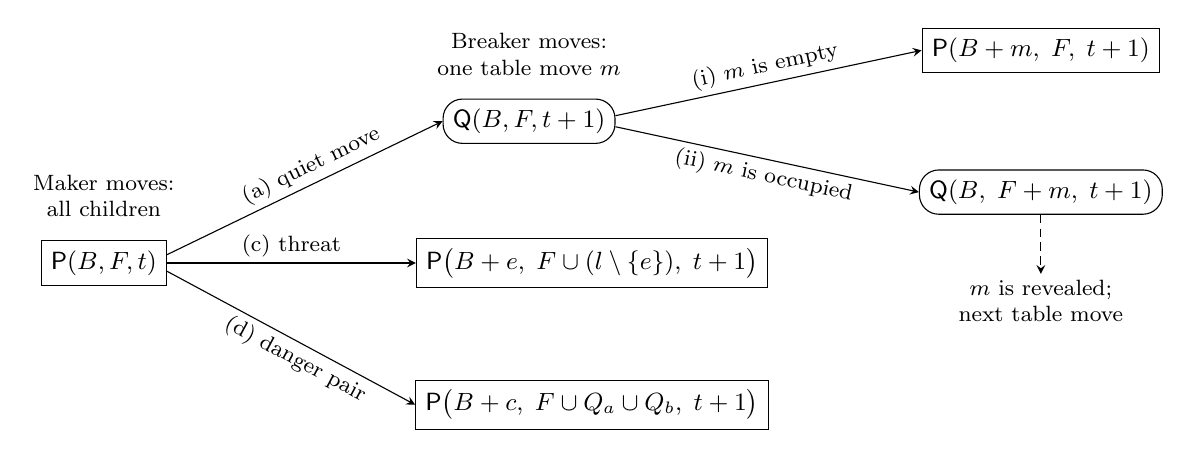
\begin{tikzpicture}[>=stealth,
    pst/.style={draw,rectangle,inner sep=3.5pt,font=\small},
    qst/.style={draw,rectangle,rounded corners=7pt,inner sep=3.5pt,font=\small},
    lbl/.style={font=\footnotesize,inner sep=2pt}]
  \node[pst] (P)  at (0,0)       {$\Pst(B,F,t)$};
  \node[qst] (Q)  at (5.4,1.8)   {$\Qst(B,F,t+1)$};
  \node[pst] (C)  at (6.2,0)     {$\Pst\bigl(B+e,\;F\cup(l\setminus\{e\}),\;t+1\bigr)$};
  \node[pst] (D)  at (6.2,-1.8)  {$\Pst\bigl(B+c,\;F\cup Q_a\cup Q_b,\;t+1\bigr)$};
  \node[pst] (I)  at (11.9,2.7)  {$\Pst(B+m,\;F,\;t+1)$};
  \node[qst] (II) at (11.9,0.9)  {$\Qst(B,\;F+m,\;t+1)$};
  \draw[->] ([yshift=3pt]P.east) -- node[lbl,sloped,above,pos=0.55] {(a) quiet move} (Q.west);
  \draw[->] (P.east) -- node[lbl,above,pos=0.5] {(c) threat} (C.west);
  \draw[->] ([yshift=-3pt]P.east) -- node[lbl,sloped,below,pos=0.55] {(d) danger pair} (D.west);
  \draw[->] ([yshift=2pt]Q.east) -- node[lbl,sloped,above] {(i) $m$ is empty} (I.west);
  \draw[->] ([yshift=-2pt]Q.east) -- node[lbl,sloped,below] {(ii) $m$ is occupied} (II.west);
  \draw[->,densely dashed] (II.south) -- ++(0,-0.75)
        node[lbl,below,align=center] {$m$ is revealed;\\ next table move};
  \node[lbl,align=center] at (0,0.85) {\Maker{} moves:\\ all children};
  \node[lbl,align=center] at (5.4,2.65) {\Breaker{} moves:\\ one table move $m$};
\end{tikzpicture}
\caption{One round of the abstract game. A P-state (\Maker{} to move, sharp corners) has one child \textup{(a)}
and one child \textup{(c)} or \textup{(d)} for every conceivable forced event; all of them must be \WON{} or
\VOID. At a Q-state (\Breaker{} to move, rounded corners) one table move $m$ is chosen; both the case that $m$
is empty and the case that $m$ holds an unrevealed stone of \Maker{} must be covered. Child \textup{(ii)} is
again a Q-state, with one more revealed stone.}
\label{fig:round}
\end{figure}

\cref{fig:round} shows one round. The children are indeed states: in \textup{(c)} we have
$e\notin B$ because $l$ is live and $e\notin F$ by assumption, so $|B+e|=t+1$ and $B+e$ is disjoint from
$F\cup(l\setminus\{e\})$; the same holds in \textup{(d)} for $c$, $Q_a$, $Q_b$; and \textup{(ii)} requires
$|F+m|\le t$. Different data may define the same child.

The meaning is as follows. In \textup{(a)}, the $(t+1)$-th move of \Maker{} has caused no forced event, and the
record does not change except for $t$. In \textup{(c)}, that move has created a threat on $l$ with sixth
cell $e$: \Breaker{} takes $e$, and the five stones on $l$ are revealed. In \textup{(d)}, it has created a
danger pair $\{a,b\}$ with common cell $c$: \Breaker{} takes $c$, and the four stones $Q_a$ on $a$ and the
four stones $Q_b$ on $b$ are revealed. The conditions $F\cap a\subseteq Q_a$, $F\cap b\subseteq Q_b$ say that
the stones already revealed on these lines are among the four, and the bounds by $t+1$ say that \Maker{}
has only $t+1$ stones at this moment. In \textup{(i)} and \textup{(ii)}, the table names the cell $m$ in round
$t$; either $m$ is empty and \Breaker{} takes it, or $m$ holds an unrevealed stone of \Maker, which is thereby
revealed. If $|F|=t$, all stones of \Maker{} are revealed, $m\notin F$ is empty, and no child \textup{(ii)} is
needed.

The lists \textup{(c)} and \textup{(d)} contain every forced event that can occur in a play
(\cref{thm:soundness}), and in general many that cannot: the definition does not ask whether the
stones can be reached by an admissible play. This only makes the requirement \WON{} below stronger. The
letter \textup{(b)} is not used here; it is reserved for an additional kind of child in the eager variant of
\cref{sec:game-remarks}.

The child \textup{(a)} of a non-\VOID{} P-state is not \VOID, and neither is the child \textup{(i)} of a
non-\VOID{} Q-state, because $F$ remains admissible when $m\notin F$ is added to $B$
(\cref{lem:adm-closed}\,(b)). Children \textup{(c)}, \textup{(d)} and \textup{(ii)} can be \VOID.

\subsection{Patterns, the predicate \texorpdfstring{$\LOST$}{LOST}, and winning states}\label{sec:won}

The following two patterns describe the situations in which a forced reply fails to restore admissibility
(\cref{lem:threat,lem:danger}). In both, $x$ plays the role of the stone that \Maker{} has
just placed, and the \emph{stone sets} are the cells that \Maker{} would hold on the lines of the pattern
after this move.

\begin{definition}[Patterns $\Etwo$ and $\Ethree$; $\LOST$]\label{def:lost}
Let $B,F$ be disjoint sets of cells and $t\ge 0$.

An \emph{$\Etwo$ pattern} for $(B,F)$ (a threat and a danger pair) consists of three pairwise distinct live
lines $l,a,b\in\live{B}$, three pairwise distinct cells $x,e,c$, and two sets $S_a,S_b$ of cells such that
\begin{enumerate}[label=\textup{(E2.\arabic*)},leftmargin=3.6em]
\item $l\cap a=\{x\}$, $e\in l$, $a\cap b=\{c\}$, $x\notin b$, $e\notin b$;
\item $S_a\subseteq a\setminus\{c\}$ with $|S_a|=4$ and $x\in S_a$; $S_b\subseteq b\setminus\{c\}$ with $|S_b|=4$;
\item $e\notin F$, $c\notin F$, $F\cap a\subseteq S_a$, $F\cap b\subseteq S_b$.
\end{enumerate}
Its stone sets are $S_l=l\setminus\{e\}$, $S_a$ and $S_b$.

An \emph{$\Ethree$ pattern} for $(B,F)$ (two danger pairs) consists of four pairwise distinct live lines
$a,a',b,b'\in\live{B}$, three pairwise distinct cells $x,c,c'$, and four sets $S_a,S_{a'},S_b,S_{b'}$ of cells
such that
\begin{enumerate}[label=\textup{(E3.\arabic*)},leftmargin=3.6em]
\item $a\cap a'=\{x\}$, $a\cap b=\{c\}$, $a'\cap b'=\{c'\}$, $x\notin b\cup b'$;
\item $S_a\subseteq a\setminus\{c\}$, $S_{a'}\subseteq a'\setminus\{c'\}$, $S_b\subseteq b\setminus\{c\}$,
  $S_{b'}\subseteq b'\setminus\{c'\}$, each of the four sets has exactly four cells, $x\in S_a\cap S_{a'}$,
  and neither $c$ nor $c'$ belongs to any of the four sets;
\item $c\notin F$, $c'\notin F$, $F\cap a\subseteq S_a$, $F\cap a'\subseteq S_{a'}$, $F\cap b\subseteq S_b$,
  $F\cap b'\subseteq S_{b'}$.
\end{enumerate}
Its stone sets are $S_a$, $S_{a'}$, $S_b$ and $S_{b'}$.

A pattern \emph{fits} $(B,F,t)$ if the union of $F$ and all stone sets of the pattern has at most $t+1$ cells.
$\LOST(B,F,t)$ holds if some $\Etwo$ pattern or some $\Ethree$ pattern for $(B,F)$ fits $(B,F,t)$.
\end{definition}

In an $\Etwo$ pattern, $l$ is a threat with sixth cell $e$, and $\{a,b\}$ is a danger pair with common cell
$c$ none of whose lines contains $e$ (note that $e\notin a$, because $e\in l$, $e\ne x$ and
$l\cap a=\{x\}$). In an $\Ethree$ pattern, $\{a,b\}$ and $\{a',b'\}$ are danger pairs with common cells $c$
and $c'$. The condition $e\notin F$ implies $F\cap l\subseteq S_l$.

\begin{definition}[\WON]\label{def:won}
Fix an integer $\Rmax\ge 0$. The label \WON{} (more precisely: \WON{} for $\Rmax$) is defined for states that
are not \VOID, by the following recursion.

A P-state $\Pst(B,F,t)$ that is not \VOID{} is \WON{} if
\begin{enumerate}[label=\textup{(P\arabic*)},leftmargin=3em]
\item $\LEAF(B,F,t)$ holds; or
\item $t<\Rmax$, $\LOST(B,F,t)$ is false, and every child \textup{(a)}, \textup{(c)}, \textup{(d)} of
  $\Pst(B,F,t)$ (\cref{def:states}) is \WON{} or \VOID.
\end{enumerate}
A Q-state $\Qst(B,F,t)$ that is not \VOID{} is \WON{} if there is a cell $m\notin B\cup F$ such that
\begin{enumerate}[label=\textup{(\roman*)},leftmargin=3em]
\item the child \textup{(i)} of $\Qst(B,F,t)$ via $m$ is \WON; and
\item if $|F|<t$, the child \textup{(ii)} of $\Qst(B,F,t)$ via $m$ is \WON{} or \VOID.
\end{enumerate}
Such a cell $m$ is called a \emph{table move} for $\Qst(B,F,t)$.
\end{definition}

In (P1) the predicate $\LEAF(B,F,k)$ of \cref{def:leaf} is used with $k=t\ge|F|$. A P-state with
$t\ge\Rmax$ is \WON{} only if it satisfies (P1). Thus $\Rmax$ bounds the number of rounds that \Breaker{} plays
from the table.

\begin{lemma}[The recursion is well founded]\label{lem:rank}
For states put
\[ \rk\bigl(\Pst(B,F,t)\bigr)=\bigl(2(\Rmax-t),\,0\bigr),\qquad
   \rk\bigl(\Qst(B,F,t)\bigr)=\bigl(2(\Rmax-t)+1,\;t-|F|\bigr), \]
and order these pairs of integers lexicographically. Then every child of a state has smaller rank than the
state itself. Consequently \cref{def:won} defines the label \WON{} uniquely for every state that is
not \VOID.
\end{lemma}

\begin{proof}
The child \textup{(a)} of $\Pst(B,F,t)$ has rank $(2(\Rmax-t)-1,\,\cdot\,)$, and the children \textup{(c)},
\textup{(d)} have rank $(2(\Rmax-t)-2,0)$; all are smaller than $(2(\Rmax-t),0)$ in the first component. The
child \textup{(i)} of $\Qst(B,F,t)$ has rank $(2(\Rmax-t),0)$, which is smaller than
$(2(\Rmax-t)+1,\,t-|F|)$ in the first component, and the child \textup{(ii)} has rank
$(2(\Rmax-t)+1,\,t-|F|-1)$, which is smaller in the second. The condition for a state to be \WON{} refers,
besides the predicates $\LEAF$ and $\LOST$ and the question which children are \VOID, only to the labels of
its children. There are finitely many
states (a state has $t\le|\Q|+1$), so the ranks form a finite totally ordered set, and the label is defined by
recursion on the rank.
\end{proof}

\subsection{Symmetry and certificates}\label{sec:cert}

For $g\in\G$ and a state $\Pst(B,F,t)$ or $\Qst(B,F,t)$, the \emph{image} under $g$ is $\Pst(gB,gF,t)$ or
$\Qst(gB,gF,t)$. The \emph{canonical form} of a state is its image under a map $g\in\G$ for which
$(gB,gF)$ is the canonical form $\canon(B,F)$ of the pair $(B,F)$ (\cref{def:canon}); we
write $\canon\Pst(B,F,t)$ and $\canon\Qst(B,F,t)$. A state is \emph{canonical} if it is its own canonical
form. The root is canonical.

\begin{lemma}[Symmetry of the abstract game]\label{lem:game-invariance}
Let $g\in\G$.
\begin{enumerate}[label=\textup{(\alph*)},leftmargin=2.4em]
\item The image of a state is a state of the same kind, with the same $t$, the same $|F|$ and the same rank.
  A state is \VOID{} if and only if its image is. Moreover $\LEAF(B,F,t)$ holds if and only if
  $\LEAF(gB,gF,t)$ holds, and $\LOST(B,F,t)$ holds if and only if $\LOST(gB,gF,t)$ holds.
\item The children \textup{(a)}, \textup{(c)}, \textup{(d)} of the image of a P-state are exactly the images
  of its children \textup{(a)}, \textup{(c)}, \textup{(d)}. The children \textup{(i)}, \textup{(ii)} of the
  image of a Q-state via $g(m)$ are the images of its children \textup{(i)}, \textup{(ii)} via $m$.
\item A state that is not \VOID{} is \WON{} if and only if its image is \WON; and $m$ is a table move for
  $\Qst(B,F,t)$ if and only if $g(m)$ is a table move for $\Qst(gB,gF,t)$.
\item A state and its image have the same canonical form.
\end{enumerate}
\end{lemma}

\begin{proof}
By \cref{lem:group}, $\G$ is a group of bijections of $\Q$ each of which maps lines onto lines.
(a) and (b): all notions involved are defined in terms of membership of cells in sets, cardinalities, and
the set of lines, and are therefore preserved by a bijection of the cells that permutes the lines. For live
lines, admissibility and $\LEAF$ this is \cref{lem:invariance}\,(a),~(b),~(e). For $\LOST$, the image of a pattern for
$(B,F)$ is a pattern for $(gB,gF)$ with stone sets of the same sizes. For (b), data $(l,e)$ define a
child \textup{(c)} of $\Pst(B,F,t)$ if and only if $(gl,g(e))$ define a child \textup{(c)} of the image, and
the second child is the image of the first; likewise for \textup{(a)}, \textup{(d)}, \textup{(i)},
\textup{(ii)}. Applying this to $g^{-1}$ shows that every child of the image arises in this way.
(c) follows from (a) and (b) by induction on the rank. (d) is \cref{lem:canon}\,(a).
\end{proof}

\begin{definition}[Certificate]\label{def:certificate}
A \emph{certificate} is a triple $(\Tbl,\Lv,\Rmax)$, where $\Rmax\ge 0$ is an integer, $\Lv$ is a finite set
of canonical P-states (the \emph{leaves}), and $\Tbl$ (the \emph{table}) is a map from a finite set of
canonical Q-states to cells. The \emph{reachable set} $V$ of the certificate is the smallest set of
canonical states such that
\begin{enumerate}[label=\textup{(R\arabic*)},leftmargin=3em,start=0]
\item the root $\Pst(\emptyset,\emptyset,0)$ belongs to $V$;
\item if a P-state $P\in V$ is not in $\Lv$, then the canonical form of every child \textup{(a)},
  \textup{(c)}, \textup{(d)} of $P$ that is not \VOID{} belongs to $V$;
\item if $Q=\Qst(B,F,t)\in V$, and $m=\Tbl(Q)$ is defined and $m\notin B\cup F$, then the canonical form of the
  child \textup{(i)} of $Q$ via $m$ belongs to $V$, and so does the canonical form of the child \textup{(ii)}
  of $Q$ via $m$ if this child exists and is not \VOID.
\end{enumerate}
The certificate is \emph{valid} if
\begin{enumerate}[label=\textup{(V\arabic*)},leftmargin=3em]
\item $\LEAF(B,F,t)$ holds for every $\Pst(B,F,t)\in V\cap\Lv$;
\item every $\Pst(B,F,t)\in V\setminus\Lv$ satisfies $t<\Rmax$, and $\LOST(B,F,t)$ is false;
\item for every $\Qst(B,F,t)\in V$, the cell $\Tbl\bigl(\Qst(B,F,t)\bigr)$ is defined and does not belong to
  $B\cup F$.
\end{enumerate}
\end{definition}

The reachable set is finite and is obtained by a search from the root; checking (V1)--(V3) along this search
is what a verifier of a certificate does (\cref{alg:verify}). Leaves and table entries outside $V$
are irrelevant.

\begin{lemma}[Certificates and \WON]\label{lem:certificate}
Let $(\Tbl,\Lv,\Rmax)$ be a certificate with reachable set $V$.
\begin{enumerate}[label=\textup{(\alph*)},leftmargin=2.4em]
\item No state of $V$ is \VOID.
\item If the certificate is valid, then every state of $V$ is \WON{} for $\Rmax$. In particular the root is
  \WON.
\item Conversely, if the root is \WON{} for $\Rmax$, then there is a valid certificate with this $\Rmax$.
\end{enumerate}
\end{lemma}

\begin{proof}
(a) The set of all canonical states that are not \VOID{} satisfies (R0)--(R2): the root is not \VOID; the
child \textup{(i)} of a Q-state that is not \VOID{} is not \VOID; all other children enter $V$ only if they
are not \VOID; and the canonical form of a state that is not \VOID{} is not \VOID{}
(\cref{lem:game-invariance}\,(a)). Since $V$ is the smallest set with (R0)--(R2), it is contained in this
set.

(b) We show by induction on the rank that every $S\in V$ is \WON. Recall that a state and its canonical form
have the same rank, and that one is \WON{} if and only if the other is (\cref{lem:game-invariance}).
If $S=\Pst(B,F,t)\in\Lv$, then $S$ satisfies (P1) by (V1). If $S=\Pst(B,F,t)\notin\Lv$, then $t<\Rmax$ and
$\LOST(B,F,t)$ is false by (V2). The canonical form of every child of $S$ that is not \VOID{} belongs to $V$
by (R1) and has smaller rank than $S$, so it is \WON{} by induction, and hence so is the child. Thus $S$
satisfies (P2). If $S=\Qst(B,F,t)$, then $m=\Tbl(S)$ is defined and $m\notin B\cup F$ by (V3). By (R2) and by
induction the child \textup{(i)} of $S$ via $m$ is \WON, and the child \textup{(ii)}, if it exists, is \VOID{}
or \WON. So $m$ is a table move for $S$, and $S$ is \WON.

(c) Let $\Lv$ be the set of all canonical P-states $\Pst(B,F,t)$ for which $\LEAF(B,F,t)$ holds, and for every
canonical Q-state that is not \VOID{} and is \WON{} choose a table move as the value of $\Tbl$. Let $W$ be
the set of all canonical states that are not \VOID{} and are \WON. We claim that $W$ satisfies (R0)--(R2),
so that $V\subseteq W$. The root belongs to $W$ by assumption. Let $P=\Pst(B,F,t)\in W\setminus\Lv$. Then
(P1) fails, so (P2) holds: every child of $P$ is \WON{} or \VOID, and the canonical form of a child that is
not \VOID{} is in $W$. Let $Q=\Qst(B,F,t)\in W$. Then $m=\Tbl(Q)$ is a table move, so $m\notin B\cup F$, the
child \textup{(i)} via $m$ is \WON, and the child \textup{(ii)}, if it exists and is not \VOID, is \WON; their
canonical forms are in $W$. This proves the claim. Now (V1) holds by the choice of $\Lv$. A P-state in
$V\setminus\Lv$ is \WON{} and violates (P1), so it satisfies (P2), which contains (V2). A Q-state in $V$ is a
canonical \WON{} state, so the table is defined there and its value is a table move, which gives (V3).
\end{proof}

\subsection{The strategy \texorpdfstring{$\sigma$}{sigma}}\label{sec:sigma}

\begin{definition}[The strategy $\sigma$]\label{def:sigma}
Let $(\Tbl,\Lv,\Rmax)$ be a certificate. \Breaker{} keeps a record $(B,F,t)$ and a \emph{mode}, which is
\TABLE{} or \PAIRING. Initially $B=F=\emptyset$, $t=0$, and the mode is \TABLE. Let $X$ always denote the set
of stones of \Maker{} on the board. Round $t+1$ (for $t=0,1,2,\dots$) runs as follows.
\begin{enumerate}[label=\textup{(S\arabic*)},leftmargin=3em]
\item\label{S:leaf} \emph{Leaf test.} If the mode is \TABLE{} and $\canon\Pst(B,F,t)\in\Lv$, then
  \Breaker{} computes a pairing $\pi$ for $(B,X)$ and switches to \PAIRING{} mode for the rest of the game.
\item\label{S:maker} \emph{Move of \Maker.} \Maker{} occupies an empty cell $x$. Put $X'=X+x$.
\item\label{S:pairing} \emph{Reply in \PAIRING{} mode.} If $x\in\pi(l)$ for a line $l\in\live{B}$ and the
  other cell of $\pi(l)$ is empty, \Breaker{} takes this other cell. Otherwise \Breaker{} takes an
  arbitrary empty cell, say the empty cell $(x_1,x_2,x_3)$ with the smallest id $36x_1+6x_2+x_3$.
\end{enumerate}
In \TABLE{} mode \Breaker{} applies the first of the following three rules that is applicable.
\begin{enumerate}[label=\textup{(S\arabic*)},leftmargin=3em,start=4]
\item\label{S:threat} \emph{Threat rule.} If some line $l\in\live{B}$ has five cells in $X'$, let $e$ be the
  sixth cell of $l$. \Breaker{} takes $e$. The new record is
  $\bigl(B+e,\;F\cup(l\setminus\{e\}),\;t+1\bigr)$.
\item\label{S:danger} \emph{Danger rule.} If $X'$ has a danger pair with respect to $B$, let $\{a,b\}$ be the
  danger pair whose common cell $c$ has the smallest id. \Breaker{} takes $c$. The new record is
  $\bigl(B+c,\;F\cup(X'\cap a)\cup(X'\cap b),\;t+1\bigr)$.
\item\label{S:table} \emph{Table rule.} Choose $g\in\G$ with $(gB,gF)=\canon(B,F)$, and put
  \[ m^{\mathrm c}=\Tbl\bigl(\Qst(gB,gF,t+1)\bigr),\qquad m=g^{-1}(m^{\mathrm c}). \]
  \begin{itemize}[leftmargin=1.5em]
  \item If $m\in X'$, replace $F$ by $F+m$ and apply \ref{S:table} again.
  \item If $m\notin X'$, \Breaker{} takes $m$. The new record is $(B+m,\;F,\;t+1)$.
  \end{itemize}
\end{enumerate}
The strategy is \emph{undefined} at a position if no pairing for $(B,X)$ exists in \ref{S:leaf}, if the table
has no entry for the Q-state in \ref{S:table}, or if the cell to be taken is not empty.
\end{definition}

Some comments are in order. In \PAIRING{} mode the record is no longer changed, and in \ref{S:pairing} the
set $B$ and the pairing $\pi$ are those of the moment of the switch. The pairs $\pi(l)$ are pairwise
disjoint, so the line $l$ in \ref{S:pairing} is unique; the proviso ``is empty'' is necessary, because the
other cell of $\pi(l)$ may already hold a stone that \Breaker{} placed earlier as an arbitrary move. In \ref{S:threat} the line $l$ is unique in all positions that matter
(\cref{lem:one-move}\,(a)); for definiteness take the first such line in a fixed order. In
\ref{S:danger} the danger pair is determined by its common cell (\cref{lem:one-move}\,(d)). In
\ref{S:table} the map $g$ need not be unique; any $g\in\G$ that attains the canonical form may be used
(\cref{lem:canon}\,(b),~(c)), and for definiteness the first one in a fixed enumeration of $\G$ is taken. With these conventions $\sigma$
prescribes at most one cell in every position, as a function of the moves played so far. The record is
changed only at the end of the round, except that \ref{S:table} may enlarge $F$ several times before a move
is found: every repetition reveals one more stone of \Maker.

\cref{thm:soundness} below shows that for a valid certificate $\sigma$ is never undefined. A pairing in
\ref{S:leaf} can be computed by a maximum flow (\cref{lem:hall}\,(c)).

\subsection{The number of stones of a pattern}\label{sec:stones}

\begin{proposition}[Stones of a pattern]\label{prop:lost-stones}
Let $B,F$ be disjoint sets of cells.
\begin{enumerate}[label=\textup{(\alph*)},leftmargin=2.4em]
\item For every $\Etwo$ pattern for $(B,F)$,
  $|S_l\cup S_a\cup S_b| = 12-|S_l\cap S_b|$ and $|S_l\cap S_b|\le 1$. Hence the stone sets of an
  $\Etwo$ pattern contain at least $11$ distinct cells.
\item For every $\Ethree$ pattern for $(B,F)$,
  \[ |S_a\cup S_{a'}\cup S_b\cup S_{b'}| \;=\; 15-|S_a\cap S_{b'}|-|S_{a'}\cap S_b|-|S_b\cap S_{b'}|, \]
  and each of the three intersections has at most one cell. Hence the stone sets of an $\Ethree$ pattern
  contain at least $12$ distinct cells.
\item $\LOST(B,F,t)$ is false whenever $t\le 9$. Consequently, in a certificate with $\Rmax\le 10$ the
  requirement ``$\LOST(B,F,t)$ is false'' of \textup{(V2)}, and of \textup{(P2)}, is satisfied automatically.
\end{enumerate}
\end{proposition}

\begin{proof}
The lines of a pattern are pairwise distinct, so any two of them have at most one common cell
(\cref{lem:geometry}).

(a) We have $|S_l|=5$ and $|S_a|=|S_b|=4$. First, $S_l\cap S_a=\{x\}$: the intersection is contained in
$l\cap a=\{x\}$, and $x$ belongs to $S_a$ by (E2.2) and to $S_l=l\setminus\{e\}$ because $x\in l$
and $x\ne e$. Second, $S_a\cap S_b=\emptyset$: the intersection is contained in $a\cap b=\{c\}$, and
$c\notin S_a$. Third, $S_l\cap S_b\subseteq l\cap b$ has at most one cell. The intersection of all three
sets is contained in $S_a\cap S_b=\emptyset$. By inclusion--exclusion,
$|S_l\cup S_a\cup S_b|=(5+4+4)-(1+0+|S_l\cap S_b|)+0$.

(b) Each of the four stone sets has four cells. Of the six pairwise intersections, $S_a\cap S_{a'}=\{x\}$,
because it is contained in $a\cap a'=\{x\}$ and $x\in S_a\cap S_{a'}$ by (E3.2); $S_a\cap S_b=\emptyset$,
because it is contained in $a\cap b=\{c\}$ and $c$ is in no stone set; and $S_{a'}\cap S_{b'}=\emptyset$ for the
same reason with $c'$. The remaining three, $S_a\cap S_{b'}$, $S_{a'}\cap S_b$ and $S_b\cap S_{b'}$, are
contained in the intersection of two distinct lines and have at most one cell each. Any three of the four
stone sets include both $S_a$ and $S_b$, or both $S_{a'}$ and $S_{b'}$; hence all intersections of three or
four of the stone sets are empty. By inclusion--exclusion the union has
$16-\bigl(1+0+0+|S_a\cap S_{b'}|+|S_{a'}\cap S_b|+|S_b\cap S_{b'}|\bigr)$ cells.

(c) If a pattern fits $(B,F,t)$, then the union of $F$ and its stone sets has at most $t+1$ cells; by (a)
and (b) this union has at least $11$ cells. So $\LOST(B,F,t)$ implies $t\ge 10$. A state
$\Pst(B,F,t)\in V\setminus\Lv$ of a certificate with $\Rmax\le 10$ that satisfies the first half of (V2) has
$t\le 9$.
\end{proof}

The bounds $11$ and $12$ are all that is needed. On the $6\times6\times6$ board the value $11$ is attained
for $\Etwo$, whereas an $\Ethree$ pattern has in fact at least $13$ distinct stones
(\cref{sec:extra-e23}). The same counting gives a cheap necessary condition, which lets an
implementation reject most states without searching for patterns: the stone sets of an $\Etwo$ pattern
contain $5-|F\cap l|$, $4-|F\cap a|$ and $4-|F\cap b|$ cells outside $F$, of which at most two coincide, so
that a fitting $\Etwo$ pattern has
$(5-|F\cap l|)+(4-|F\cap a|)+(4-|F\cap b|)-2\le t+1-|F|$.

\subsection{One move of \texorpdfstring{\Maker}{Maker} from an admissible position}\label{sec:one-move}

The next three lemmas analyze what a single move of \Maker{} can do to an admissible position. They are the
link between real plays and the children \textup{(c)}, \textup{(d)} and the patterns $\Etwo$, $\Ethree$.

\begin{lemma}[One move]\label{lem:one-move}
Let $X$ be $B$-admissible, let $x\notin B\cup X$ be a cell, and let $X'=X+x$. Threats and danger pairs refer
to $B$.
\begin{enumerate}[label=\textup{(\alph*)},leftmargin=2.4em]
\item No live line has six cells in $X'$. At most one live line has five cells in $X'$; such a line contains
  $x$.
\item In every danger pair of $X'$ exactly one of the two lines contains $x$. This line, the \emph{new line}
  of the pair, has exactly three cells in $X$. The other line, the \emph{old line} of the pair, has exactly
  four cells in $X$. The common cell $c$ of the pair is different from $x$ and is empty, that is,
  $c\notin B\cup X'$.
\item Two distinct old lines of danger pairs of $X'$ have no common cell outside $X'$. Two distinct new
  lines of danger pairs of $X'$ have exactly the cell $x$ in common.
\item Distinct danger pairs of $X'$ have distinct common cells.
\end{enumerate}
\end{lemma}

\noindent In the sequel a danger pair of $X'$ is written as an ordered pair $(a,b)$, with $a$ its new line and
$b$ its old line.

\begin{proof}
(a) A live line has at most four cells in $X$, hence at most five in $X'$, and exactly five only if it
contains $x$ and has exactly four cells in $X$. Two distinct live lines of this kind would share the cell
$x\notin X$ and would form a danger pair of $X$, which does not exist.

(b) Let $\{a,b\}$ be a danger pair of $X'$ with common cell $c\notin X'$. If neither line contained $x$,
then $a\cap X=a\cap X'$ and $b\cap X=b\cap X'$ would have four cells each, and $c\notin X$: a danger pair of
$X$. If both lines contained $x$, then $a\cap b=\{x\}$ by \cref{lem:geometry}, so $c=x\in X'$, which is
false. So exactly one line contains $x$; it has $4-1=3$ cells in $X$, and the other line has four cells in
$X$. Finally $c\ne x$ because $c\notin X'$, and $c\notin B$ because the lines are live.

(c) An old line has exactly four cells in $X$ by (b). If two distinct old lines had a common cell outside
$X'\supseteq X$, they would form a danger pair of $X$. Two distinct new lines both contain $x$, and they have
no other common cell by \cref{lem:geometry}.

(d) Let $(a,b)$ and $(a',b')$ be danger pairs of $X'$ with the same common cell $c$. The new lines $a$ and
$a'$ both contain the two distinct cells $x$ and $c$, so $a=a'$ by \cref{lem:geometry}. The old lines $b$
and $b'$ both contain $c\notin X'$, so $b=b'$ by (c).
\end{proof}

\begin{lemma}[Threat]\label{lem:threat}
Let $X$ be $B$-admissible, $F\subseteq X$ and $t=|X|$. Let $x\notin B\cup X$ and $X'=X+x$. Suppose that a live
line $l\in\live{B}$ has five cells in $X'$, and let $e$ be its sixth cell. Then $e$ is empty, and one of the
following holds:
\begin{enumerate}[label=\textup{(\arabic*)},leftmargin=2.4em]
\item $X'$ is $(B+e)$-admissible; or
\item some $\Etwo$ pattern for $(B,F)$ fits $(B,F,t)$, so that $\LOST(B,F,t)$ holds.
\end{enumerate}
\end{lemma}

\begin{proof}
We have $e\notin X'$ by the choice of $e$, and $e\notin B$ because $l$ is live. Hence $e$ is empty and
$X'\cap(B+e)=\emptyset$. The lines that are live with respect to $B+e$ are the lines of $\live{B}$ that do
not contain $e$. By \cref{lem:one-move}\,(a), $l$ is the only line of $\live{B}$ with more than four
cells in $X'$, and $l$ contains $e$. So every line that is live with respect to $B+e$ has at most four
cells in $X'$.

Suppose that (1) fails. Then $X'$ has a danger pair with respect to $B+e$. This is a danger pair $(a,b)$ of
$X'$ with respect to $B$ such that $e\notin a\cup b$; let $a$ be its new line, $b$ its old line and $c$ its
common cell (\cref{lem:one-move}\,(b)). We verify that the lines $l,a,b$, the cells $x,e,c$ and the sets
$S_a=X'\cap a$, $S_b=X'\cap b$ form an $\Etwo$ pattern for $(B,F)$. The three lines are live with respect to
$B$. They are pairwise distinct: $a\ne b$, and $e$ lies on $l$ but not on $a$ or $b$. The three cells are
pairwise distinct: $x\in X'$ whereas $e,c\notin X'$, and $c\in a$ whereas $e\notin a$.
\begin{itemize}[leftmargin=2.2em]
\item (E2.1): $x\in l$ by \cref{lem:one-move}\,(a) and $x\in a$, so $l\cap a=\{x\}$ by
  \cref{lem:geometry}; $e\in l$; $a\cap b=\{c\}$ by \cref{lem:geometry}; $x\notin b$ because $b$ is
  the old line; $e\notin b$.
\item (E2.2): $S_a$ and $S_b$ have four cells each because $(a,b)$ is a danger pair of $X'$; they do not
  contain $c$ because $c\notin X'$; and $x\in S_a$.
\item (E2.3): $F\subseteq X\subseteq X'$, hence $e\notin F$, $c\notin F$, $F\cap a\subseteq X'\cap a=S_a$
  and $F\cap b\subseteq S_b$.
\end{itemize}
The stone sets are $S_l=l\setminus\{e\}=X'\cap l$, $S_a$ and $S_b$. Their union with $F$ is contained
in $X'$ and therefore has at most $|X'|=t+1$ cells: the pattern fits $(B,F,t)$.
\end{proof}

\begin{lemma}[Danger]\label{lem:danger}
Let $X$ be $B$-admissible, $F\subseteq X$ and $t=|X|$. Let $x\notin B\cup X$ and $X'=X+x$. Suppose that no live
line has five cells in $X'$ and that $X'$ has at least one danger pair with respect to $B$. Let $(a,b)$ be
\emph{any} danger pair of $X'$, and let $c$ be its common cell. Then $c$ is empty, and one of the following
holds:
\begin{enumerate}[label=\textup{(\arabic*)},leftmargin=2.4em]
\item $X'$ is $(B+c)$-admissible; or
\item some $\Ethree$ pattern for $(B,F)$ fits $(B,F,t)$, so that $\LOST(B,F,t)$ holds.
\end{enumerate}
More precisely, if no $\Ethree$ pattern fits $(B,F,t)$, then any two danger pairs of $X'$ have a line in
common, and either all danger pairs of $X'$ have the same new line or all of them have the same old line.
\end{lemma}

\begin{proof}
The cell $c$ is empty by \cref{lem:one-move}\,(b), so $X'\cap(B+c)=\emptyset$. By
\cref{lem:one-move}\,(a) and the hypothesis, every line of $\live{B}$ has at most four cells in $X'$. The
lines that are live with respect to $B+c$ are the lines of $\live{B}$ that do not contain $c$. Therefore
$X'$ is $(B+c)$-admissible unless there is a danger pair of $X'$ with respect to $B$ none of whose lines
contains $c$.

Let $(a',b')$ be a danger pair of $X'$ with respect to $B$ such that $a'\ne a$ and $b'\ne b$, and let $c'$ be
its common cell. We verify that the lines $a,a',b,b'$, the cells $x,c,c'$ and the sets $S_a=X'\cap a$,
$S_{a'}=X'\cap a'$, $S_b=X'\cap b$, $S_{b'}=X'\cap b'$ form an $\Ethree$ pattern for $(B,F)$. The four lines are
live with respect to $B$. They are pairwise distinct: $a\ne a'$ and $b\ne b'$ by assumption, and the new
lines $a,a'$ contain $x$ while the old lines $b,b'$ do not. The three cells are pairwise distinct: $x\in X'$
whereas $c,c'\notin X'$, and $c\ne c'$ by \cref{lem:one-move}\,(d).
\begin{itemize}[leftmargin=2.2em]
\item (E3.1): $a\cap a'=\{x\}$ by \cref{lem:one-move}\,(c); $a\cap b=\{c\}$ and $a'\cap b'=\{c'\}$ by
  \cref{lem:geometry}; $x\notin b\cup b'$ because $b$ and $b'$ are old lines.
\item (E3.2): each of the four sets has four cells because the lines belong to danger pairs of $X'$; the
  sets do not contain $c$ or $c'$ because $c,c'\notin X'$, and in particular they are contained in
  $a\setminus\{c\}$, $a'\setminus\{c'\}$, $b\setminus\{c\}$, $b'\setminus\{c'\}$, respectively; and
  $x\in S_a\cap S_{a'}$.
\item (E3.3): $F\subseteq X\subseteq X'$, hence $c,c'\notin F$ and $F\cap a\subseteq X'\cap a=S_a$, and
  likewise for $a'$, $b$, $b'$.
\end{itemize}
The union of $F$ and the four stone sets is contained in $X'$ and has at most $t+1$ cells: the pattern fits
$(B,F,t)$.

Now suppose that no $\Ethree$ pattern fits $(B,F,t)$. By what was just shown, every danger pair $(a',b')$ of
$X'$ has $a'=a$ or $b'=b$, so one of its lines contains $c\in a\cap b$. Hence no danger pair of $X'$ with
respect to $B$ avoids $c$, and (1) holds. Since $(a,b)$ was arbitrary, any two danger pairs have a line in
common: the new line or the old line, and not both if the pairs are different. If two different pairs have
the same new line $a_1$, so that their old lines $b_1\ne b_2$ differ, then a pair with a new line different
from $a_1$ would have to have the old line $b_1$ and the old line $b_2$, which is impossible; so all pairs
have the new line $a_1$. Otherwise no two different pairs have the same new line, and then any two pairs
have the same old line.
\end{proof}

\begin{remark}[At most one forced event with ten stones]\label{rem:one-event}
In the situation of \cref{lem:one-move} suppose that $|X'|\le 10$. Then $X'$ has no threat and no danger
pair, or exactly one threat and no danger pair, or no threat and exactly one danger pair. Indeed, there is
at most one threat by \cref{lem:one-move}\,(a). A threat $l$ together with a danger pair $(a,b)$
requires at least $5+4+4-2=11$ stones, since $l\cap a=\{x\}$ (both lines contain $x$, and they are
distinct because they have different numbers of cells in $X'$), the common cell of $a$ and $b$ is not in
$X'$, and $l$ and $b$ share at most one cell. Two danger pairs with the same new line $a$ and old lines
$b\ne b'$ require at least $4+4+4-1=11$ stones, since the cells $a\cap b$ and $a\cap b'$ are not in $X'$ and
$b$, $b'$ share at most one cell. Two danger pairs with new lines $a\ne a'$ and the same old line $b$ require
$(4+4-1)+4=11$ stones, since $a\cap a'=\{x\}$ and the cells $a\cap b$, $a'\cap b$ are not in $X'$. Two danger
pairs with different new lines and different old lines require at least $12$ stones by the proof of
\cref{lem:danger} and \cref{prop:lost-stones}\,(b). Consequently, when \Breaker{} follows $\sigma$ for a valid certificate with $\Rmax\le 10$, the forced reply
in \TABLE{} mode is always unique and the choice in rule \ref{S:danger} is never exercised: there $X$ is
$B$-admissible and $|X'|=t+1\le\Rmax$ by \cref{thm:soundness} below.
\end{remark}

\subsection{Soundness}\label{sec:soundness}

\begin{theorem}[Soundness of the abstract game]\label{thm:soundness}
Let $(\Tbl,\Lv,\Rmax)$ be a valid certificate with reachable set $V$, and let \Breaker{} play the strategy
$\sigma$ of \cref{def:sigma} against arbitrary moves of \Maker. Consider a round that begins in
\TABLE{} mode. Let $t$ be the number of completed rounds, $X$ the set of stones of \Maker, and $(B,F,t)$ the
record of \Breaker{} at the beginning of this round. Then:
\begin{enumerate}[label=\textup{(I\arabic*)},leftmargin=3em]
\item\label{I:V} $\canon\Pst(B,F,t)\in V$; in particular $\Pst(B,F,t)$ is not \VOID{} and is \WON;
\item\label{I:B} $B$ is exactly the set of stones of \Breaker, and $|B|=t$;
\item\label{I:F} $F\subseteq X$ and $|X|=t$;
\item\label{I:adm} $X$ is $B$-admissible.
\end{enumerate}
Moreover, in this round $\sigma$ is defined: if $\canon\Pst(B,F,t)\in\Lv$, then a pairing for $(B,X)$ exists;
otherwise $t<\Rmax$, and after the move of \Maker{} the rules \ref{S:threat}--\ref{S:table} yield a cell that
is empty, where every look-up in rule \ref{S:table} finds a table entry and rule \ref{S:table} is repeated
at most $t+1-|F|$ times.
\end{theorem}

\begin{proof}
We use induction on $t$. For $t=0$ we have $B=F=X=\emptyset$, the root belongs to $V$, and
\ref{I:V}--\ref{I:adm} hold. Now consider a round that begins in \TABLE{} mode and for which
\ref{I:V}--\ref{I:adm} hold. We show that $\sigma$ is defined in this round, and that
\ref{I:V}--\ref{I:adm} hold at the beginning of the next round unless $\sigma$ has switched to \PAIRING{} mode.
Choose $g\in\G$ with $(gB,gF)=\canon(B,F)$, and let $P^{\mathrm c}=\Pst(gB,gF,t)$, which belongs to $V$
by \ref{I:V}. That $\Pst(B,F,t)$ is not \VOID{} and is \WON{} follows from
\cref{lem:certificate}\,(a),~(b) and \cref{lem:game-invariance}.

\smallskip\noindent\emph{Leaf.} Suppose $P^{\mathrm c}\in\Lv$. By (V1), $\LEAF(gB,gF,t)$ holds, hence
$\LEAF(B,F,t)$ holds (\cref{lem:game-invariance}\,(a)), and hence $\CC(B,F,t)$ holds
(\cref{thm:leaf-implies-C}): every $B$-admissible set that contains $F$ and has at most $t$ cells has
a pairing. By \ref{I:F} and \ref{I:adm}, $X$ is such a set. So a pairing for $(B,X)$ exists, rule
\ref{S:leaf} is defined, and $\sigma$ switches to \PAIRING{} mode. Nothing more is claimed in this case; from
here on the pairing strategy of \cref{lem:pairing} takes over (see the proof of
\cref{thm:sigma}).

\smallskip\noindent\emph{Expanded state.} Suppose $P^{\mathrm c}\notin\Lv$. By (V2) and
\cref{lem:game-invariance}\,(a), $t<\Rmax$ and
\begin{equation}\label{eq:notlost}
  \LOST(B,F,t)\ \text{is false.}
\end{equation}
By (R1), the canonical form of every child \textup{(a)}, \textup{(c)}, \textup{(d)} of $P^{\mathrm c}$ that is
not \VOID{} belongs to $V$. By \cref{lem:game-invariance}\,(a),~(b),~(d) these canonical forms are exactly the
canonical forms of the children of $\Pst(B,F,t)$ that are not \VOID. Thus
\begin{equation}\label{eq:children}
  \begin{minipage}{0.84\textwidth}\centering
  the canonical form of every child \textup{(a)}, \textup{(c)}, \textup{(d)} of $\Pst(B,F,t)$\\
  that is not \VOID{} belongs to $V$.
  \end{minipage}
\end{equation}
If the board is full, the game is over. Otherwise \Maker{} occupies an empty cell $x$. Let $X'=X+x$; then $|X'|=t+1$ and $x\notin B\cup X$ by \ref{I:B}, so
\crefrange{lem:one-move}{lem:danger} apply to $B$, $X$, $F$, $t$ and $x$. Exactly one of the following
three cases occurs, and $\sigma$ distinguishes them by the rules \ref{S:threat}, \ref{S:danger},
\ref{S:table}.

\smallskip\noindent\emph{Case 1: some live line has five cells in $X'$.} By \cref{lem:one-move}\,(a) this
line $l$ is unique. Rule \ref{S:threat} prescribes its sixth cell $e$, which is empty by
\cref{lem:threat}. The new record is $(B',F',t+1)$ with $B'=B+e$ and $F'=F\cup(l\setminus\{e\})$. By
\eqref{eq:notlost} and \cref{lem:threat}, $X'$ is $B'$-admissible. The state $\Pst(B',F',t+1)$ is a child
\textup{(c)} of $\Pst(B,F,t)$, defined by $l$ and $e$: the line $l$ is live; $e\in l\setminus F$
because $e\notin X'\supseteq F$; and $F\cup(l\setminus\{e\})\subseteq X'$, since
$l\setminus\{e\}=X'\cap l$, so this set has at most $t+1$ cells. This child is not \VOID, because
$F'\subseteq X'$ and $X'$ is $B'$-admissible (\cref{lem:adm-closed}\,(a)). By \eqref{eq:children} its
canonical form belongs to $V$. Hence \ref{I:V}--\ref{I:adm} hold at the beginning of the next round, with
$(B',F',t+1)$ and $X'$.

\smallskip\noindent\emph{Case 2: no live line has five cells in $X'$, and $X'$ has a danger pair.} Rule
\ref{S:danger} selects a danger pair $(a,b)$ with common cell $c$ and prescribes $c$, which is empty by
\cref{lem:danger}. The new record is $(B',F',t+1)$ with $B'=B+c$ and
$F'=F\cup(X'\cap a)\cup(X'\cap b)$. By \eqref{eq:notlost} and \cref{lem:danger}, $X'$ is $B'$-admissible.
The state $\Pst(B',F',t+1)$ is a child \textup{(d)} of $\Pst(B,F,t)$, defined by $a$, $b$, $Q_a=X'\cap a$ and
$Q_b=X'\cap b$: the lines $a\ne b$ are live and $a\cap b=\{c\}$; $c\notin F$ and $c\notin Q_a\cup Q_b$ because
$c\notin X'\supseteq F$; $|Q_a|=|Q_b|=4$ by the definition of a danger pair; $F\cap a\subseteq Q_a$ and
$F\cap b\subseteq Q_b$ because $F\subseteq X'$; and $F\cup Q_a\cup Q_b\subseteq X'$ has at most $t+1$ cells.
This child is not \VOID, because $F'\subseteq X'$ and $X'$ is $B'$-admissible. By \eqref{eq:children} its
canonical form belongs to $V$, and \ref{I:V}--\ref{I:adm} hold at the beginning of the next round.

\smallskip\noindent\emph{Case 3: no live line has five cells in $X'$, and $X'$ has no danger pair.} Then $X'$
is $B$-admissible: it is disjoint from $B$, no live line has more than four cells in $X'$
(\cref{lem:one-move}\,(a)), and there is no danger pair. Now $\sigma$ applies rule \ref{S:table}, possibly
several times. We claim that each time rule \ref{S:table} is entered, the current set $F$ satisfies
\begin{equation}\label{eq:loop}
  \canon\Qst(B,F,t+1)\in V\qquad\text{and}\qquad F\subseteq X'.
\end{equation}
At the first entry, $F\subseteq X\subseteq X'$, and $\Qst(B,F,t+1)$ is the child \textup{(a)} of
$\Pst(B,F,t)$, which is not \VOID; so \eqref{eq:loop} holds by \eqref{eq:children}. Suppose \eqref{eq:loop}
holds at some entry. Let $g'\in\G$ be the map chosen by the rule, so that
$Q^{\mathrm c}=\Qst(g'B,g'F,t+1)$ is the canonical form of $\Qst(B,F,t+1)$ and belongs to $V$. By (V3) the
table entry $m^{\mathrm c}=\Tbl(Q^{\mathrm c})$ exists and $m^{\mathrm c}\notin g'B\cup g'F$; hence
$m=g'^{-1}(m^{\mathrm c})\notin B\cup F$. By (R2) and \cref{lem:game-invariance}\,(b),~(d), the canonical
form of the child \textup{(i)} of $\Qst(B,F,t+1)$ via $m$ belongs to $V$, and so does the canonical form of
its child \textup{(ii)} via $m$ if this child exists and is not \VOID.
\begin{itemize}[leftmargin=2.2em]
\item If $m\in X'$, then $m\in X'\setminus F$, so $|F|<|X'|=t+1$ and the child \textup{(ii)},
  $\Qst(B,F+m,t+1)$, exists. It is not \VOID, because $F+m\subseteq X'$ and $X'$ is $B$-admissible
  (\cref{lem:adm-closed}\,(a)). So \eqref{eq:loop} holds for $F+m$, with which the rule is entered again.
  Every such step moves a cell of $X'\setminus F$ into $F$, so there are at most $|X'\setminus F|$ of them,
  counted from the first entry; this number is $t+1-|F|$ for the set $F$ at the beginning of the round.
\item If $m\notin X'$, then $m$ is empty, because $m\notin B$ and $B$ is the set of all stones of \Breaker{}
  by \ref{I:B}. \Breaker{} takes $m$, and the new record is $(B+m,F,t+1)$, where $F$ is the current set. The
  canonical form of the child \textup{(i)}, $\Pst(B+m,F,t+1)$, belongs to $V$; this is \ref{I:V}. Clearly
  \ref{I:B} holds; \ref{I:F} holds by \eqref{eq:loop} and $|X'|=t+1$; and $X'$ is $(B+m)$-admissible because
  it is $B$-admissible and $m\notin X'$ (\cref{lem:adm-closed}\,(b)), which is \ref{I:adm}.
\end{itemize}
In all three cases $\sigma$ was defined, the cell prescribed was empty, and \ref{I:V}--\ref{I:adm} hold at the
beginning of the next round.
\end{proof}

Three features of the proof deserve to be pointed out. All cardinality conditions in the definitions of the
children \textup{(c)}, \textup{(d)}, \textup{(ii)} and of the patterns were verified in the same way: the
sets in question are subsets of $X'$, and $|X'|=t+1$. A \VOID{} child is never entered, since the revealed set
is always a subset of the real set $X'$ of stones of \Maker, which is admissible with respect to the new set
of stones of \Breaker. And the proof does not use any property of the cells named by the table, nor the
particular choice of the danger pair in rule \ref{S:danger}, nor the choice of $g$ in rule \ref{S:table}.

\subsection{Proof of \texorpdfstring{\cref{thm:main}}{the main theorem}}\label{thm:main-proof}

We first state precisely what the strategy $\sigma$ achieves.

\begin{theorem}[The strategy $\sigma$]\label{thm:sigma}
Let $(\Tbl,\Lv,\Rmax)$ be a valid certificate, and let \Breaker, moving second, play the strategy $\sigma$ of
\cref{def:sigma}. Then, whatever \Maker{} plays:
\begin{enumerate}[label=\textup{(\alph*)},leftmargin=2.4em]
\item whenever \Breaker{} is to move, $\sigma$ prescribes a cell, and this cell is empty;
\item at no moment does \Maker{} own all six cells of a line;
\item \Breaker{} makes at most $\Rmax$ moves in \TABLE{} mode; from round $\Rmax+1$ on, $\sigma$ is in
  \PAIRING{} mode.
\end{enumerate}
\end{theorem}

\begin{proof}
Consider a round that begins in \TABLE{} mode, with $t$ completed rounds, and use the notation and the
statements \ref{I:V}--\ref{I:adm} of \cref{thm:soundness}.

(c) If $\sigma$ does not switch to \PAIRING{} mode in this round, then $\canon\Pst(B,F,t)\in V\setminus\Lv$,
and $t<\Rmax$ by (V2). So a round that begins in \TABLE{} mode after $\Rmax$ completed rounds switches to
\PAIRING{} mode at once.

(a), (b) in \TABLE{} mode. By \cref{thm:soundness} the strategy is defined in this round and
prescribes an empty cell. A line that is not live contains a stone of \Breaker{} by \ref{I:B}. Before the
move of \Maker, a live line has at most four cells in $X$ by \ref{I:adm}; after it, at most five
(\cref{lem:one-move}\,(a)). So \Maker{} owns no line, neither after the move of \Maker{} nor after the
reply of \Breaker.

(a), (b) in \PAIRING{} mode. Suppose that $\sigma$ switches to \PAIRING{} mode at the beginning of a round,
after $t$ completed rounds. At this moment \Maker{} is to move, $B$ is the set of all stones of \Breaker,
$|B|=|X|=t$ by \ref{I:B} and \ref{I:F}, and $\sigma$ holds a pairing $\pi$ for $(B,X)$, which exists by
\cref{thm:soundness}. From now on $\sigma$ replies by rule \ref{S:pairing}: the other cell of
$\pi(l)$ if \Maker{} has taken a cell of $\pi(l)$ and that other cell is empty, and an arbitrary empty
cell otherwise. This is the situation of \cref{lem:pairing}, which states that this rule always names
an empty cell and that \Maker{} never owns all six cells of a line.
\end{proof}

The second assertion of \cref{thm:main} concerns the ordinary game, in which each player tries to be
the first to own a line. It follows from \cref{thm:sigma} by the classical strategy-stealing argument; see, for
example, \cite{Beck2008} or \cite[Theorem~3.1]{Krivelevich2014}. We include a proof, because the argument is
short and its details are often left to the reader.

\begin{proposition}[Strategy stealing]\label{prop:stealing}
Consider a game on a finite non-empty set of cells with a family $\mathcal{W}$ of non-empty subsets, the
\emph{winning sets}: two
players alternately occupy an empty cell; the player who first owns all cells of a winning set wins and the
game ends; if all cells are occupied and no player owns a winning set, the game is a draw. In such a game the
second player has no winning strategy.
\end{proposition}

\begin{proof}
A \emph{winning strategy} for a player is a strategy such that every play in which this player follows it
ends with a win of this player. Suppose that $\tau$ is a winning strategy for the second player. We describe
a strategy $\tau^*$ for the first player and show that it is winning. This is a contradiction, since a play in
which the first player follows $\tau^*$ and the second player follows $\tau$ cannot be won by both.

Under $\tau^*$ the first player imagines, besides the real play, a \emph{virtual play} of the same game, in
which the moves of the virtual first player are the moves of the real second player and the virtual second
player follows $\tau$. In addition one stone of the real first player is marked as the \emph{ghost}; let $z$
be its cell. The first real move is an arbitrary cell, which becomes the ghost; at this moment no move has
been made in the virtual play. We maintain the following invariant at all moments at which the real first
player has just moved:
\begin{itemize}[leftmargin=2.2em]
\item[$(\ast)$] the stones of the virtual first player are exactly the stones of the real second player; the
  stones of the virtual second player are exactly the stones of the real first player other than the ghost;
  and in the virtual play the first player is to move.
\end{itemize}
At all moments considered below, the stones of each virtual player are among the stones of a real player,
and the cell $z$ is empty in the virtual position. Hence, whenever the real game is not over, the virtual
game is not over either: nobody owns a winning set in the virtual position, and the virtual board is not
full. Suppose $(\ast)$ holds, the real game is not over, and the real second player
occupies a cell $y$ after which the real game is still not over. The cell $y$ is empty in the virtual
position as well, and the virtual first player occupies $y$. Since the virtual game is still not over,
$\tau$ prescribes a cell $w$ that is empty in the virtual position.
Either $w\ne z$; then $w$ is empty on the real board, and the real first player occupies $w$. Or $w=z$; then
the real first player occupies an arbitrary empty cell $z'$ of the real board, which exists because the real
game is not over, and $z'$ becomes the ghost, while the stone on $z$ is no longer marked. In both cases the
virtual second player occupies $w$, and $(\ast)$ holds again. By construction the virtual play is a play of the
game in which the second player follows $\tau$.

Now consider a real play in which the first player follows $\tau^*$, continued until the game ends. If it
ends because the first player owns a winning set, the first player wins, as desired. We show that the two
other endings are impossible.

Suppose the play ends because the second player owns a winning set after a move $y$. Let the virtual first
player occupy $y$. Then the virtual first player owns a winning set, while the virtual second player, whose
stones are among those of the real first player, has not owned a winning set at any time. So the virtual
play, in which the second player follows $\tau$, is won by the first player. This contradicts the choice of
$\tau$.

Suppose the play ends with a full board on which nobody owns a winning set. If the last move $y$ was made
by the second player, let the virtual first player occupy $y$. Then $z$ is the only empty cell of the virtual
position, nobody owns a winning set there, and $\tau$ prescribes $w=z$. After this virtual move the virtual
board is full, and each virtual player has exactly the stones of a real player; so the virtual play, in
which the second player follows $\tau$, ends in a draw. If the last move was made by the first player, then
by $(\ast)$ the cell $z$ is the only empty cell of the virtual position and the virtual first player is to
move. Let the virtual first player occupy $z$. Then the virtual board is full, and the virtual second
player, whose stones are among those of the real first player, owns no winning set; so this virtual play, in
which the second player follows $\tau$, is not won by the second player. Both cases contradict the choice of
$\tau$.
\end{proof}

\begin{corollary}[Draw]\label{cor:draw}
Suppose that there is a valid certificate. Then ordinary $6\times6\times6$ tic-tac-toe is a draw: each player
has a strategy with which this player never loses. For the second player, $\sigma$ is such a strategy.
\end{corollary}

\begin{proof}
The ordinary game is the game of \cref{prop:stealing} with the $148$ lines as winning sets. If the
second player follows $\sigma$, the first player never owns a line (\cref{thm:sigma}), so the second
player does not lose; the play ends when the second player owns a line or when the board is full. In
particular the first player has no winning strategy. The second player has no winning strategy either, by
\cref{prop:stealing}. The game is finite and has perfect information, so by Zermelo's theorem~\cite{Zermelo1913}
(backward induction on the game tree) one of the players has a winning strategy or both players have
strategies with which they never lose. Hence the first player also has a strategy with which
the first player never loses.
\end{proof}

\begin{proof}[Proof of \cref{thm:main}]
Suppose that the root $\Pst(\emptyset,\emptyset,0)$ is \WON{} for some $\Rmax$. Then there is a valid
certificate $(\Tbl,\Lv,\Rmax)$, by \cref{lem:certificate}\,(c). Let $\sigma$ be the strategy of
\cref{def:sigma} for this certificate, played by \Breaker{} as the second player. By
\cref{thm:sigma}, $\sigma$ prescribes an empty cell whenever \Breaker{} is to move, and \Maker{} never
owns all six cells of a line. By \cref{cor:draw}, the ordinary game is a draw. For $\Rmax=10$ the
hypothesis is \cref{fact:H}.
\end{proof}

The proof uses exactly one computed statement, \cref{fact:H}. In particular the geometric facts
it relies on (\cref{lem:geometry,lem:group}) are proved by hand, and by
\cref{prop:lost-stones}\,(c) the predicate $\LOST$ plays no role for $\Rmax=10$: validity of a
certificate with $\Rmax=10$ amounts to (V1), the inequality $t<\Rmax$ in (V2), and (V3).

\subsection{Remarks}\label{sec:game-remarks}

\begin{remark}[$\LOST$ is conservative; the choice of the danger pair is immaterial]\label{rem:conservative}
(i) By \cref{lem:danger}, if $\LOST(B,F,t)$ is false, then the common cell of \emph{every} danger pair
restores admissibility. So the rule ``smallest id'' in \ref{S:danger} can be replaced by any other rule
without affecting \cref{thm:soundness,thm:sigma}.

(ii) The patterns are necessary for the failure of a forced reply, not sufficient. \cref{lem:threat,lem:danger} show that a pattern fits whenever a forced reply does not restore admissibility. The
converse fails for $\Ethree$: if the danger pairs of $X'$ are exactly $(a,b)$, $(a',b')$ and $(a,b')$ with
$a\ne a'$ and $b\ne b'$, then an $\Ethree$ pattern fits by the proof of \cref{lem:danger}, applied to
$(a,b)$ and $(a',b')$, although the common cell of $(a,b')$ lies on a line of each of the three pairs, so
that \Breaker{} restores admissibility by taking it. \cref{ex:conservative} in \cref{sec:extra-e23} shows that this happens.
Moreover $\LOST(B,F,t)$ is a statement about the record: it asks whether the stones of a pattern can be
accommodated numerically, not whether they can arise in a play. In both respects the abstract game declares
more states lost than necessary. This makes the hypothesis ``the root is \WON'' harder to satisfy and is
harmless for soundness, which uses only the implications proved in \cref{lem:threat,lem:danger}.

(iii) By \cref{prop:lost-stones}\,(c) and \cref{rem:one-event}, neither (i) nor (ii) matters
for a certificate with $\Rmax\le 10$.
\end{remark}


The abstract game is monotone in the revealed set: revealing more stones never hurts \Breaker. This is not
needed for \cref{thm:main}, but it clarifies the relation between lazy revelation and variants in
which more information is used. The proofs of the next two statements are given in
\cref{sec:extra-lazy}.

\begin{proposition}[Lazy monotonicity]\label{prop:lazy-monotone}
Fix $\Rmax$. Let $F\subseteq F'$, where $F'$ is $B$-admissible and $|F'|\le t$.
\begin{enumerate}[label=\textup{(\alph*)},leftmargin=2.4em]
\item If the P-state $\Pst(B,F,t)$ is \WON, then $\Pst(B,F',t)$ is \WON.
\item If the Q-state $\Qst(B,F,t)$ is \WON, then $\Qst(B,F',t)$ is \WON.
\end{enumerate}
\end{proposition}

In an \emph{eager} variant of the abstract game, a stone that \Maker{} places on a cell of a fixed set
$H\subseteq\Q$ is revealed at once; the natural choice for $H$ is the set $\Busy$ of the $24$ busy cells. Formally, let the label $\WONp$ be defined like \WON{} in
\cref{def:won}, with the same $\Rmax$ and with the following additional requirement in (P2):
\begin{enumerate}[leftmargin=2.6em]
\item[\textup{(b)}] for every cell $h\in H\setminus(B\cup F)$, the Q-state $\Qst(B,F+h,t+1)$ is $\WONp$ or
  \VOID.
\end{enumerate}
The recursion is well founded by the rank of \cref{lem:rank}, since $\Qst(B,F+h,t+1)$ has smaller rank
than $\Pst(B,F,t)$.

\begin{corollary}[Eager variant]\label{cor:eager}
For every set $H\subseteq\Q$, every state that is \WON{} is $\WONp$. In particular, if the root is \WON{} for
$\Rmax$, then it is $\WONp$ for $\Rmax$.
\end{corollary}

\begin{remark}[Lazy versus eager]\label{rem:eager}
The label $\WONp$ keeps all requirements of \WON{} and adds the children \textup{(b)}. In a game in which
every stone of \Maker{} on $H$ is really revealed at once, requirement \textup{(ii)} would be void for table
moves $m\in H$, because an unrevealed stone never lies on $H$; so $\WONp$ is at least as demanding as such a
game. \cref{cor:eager} thus says that a lazy certificate is the stronger statement. The converse is
not claimed, and the eager variant was not investigated computationally. In terms of strategies, eager
revelation is the special case of lazy revelation in which \Breaker{} inspects all cells of $H$ after every
move of \Maker: at any time \Breaker{} may replace $F$ in the record by a set $F'$ with
$F\subseteq F'\subseteq X$. The statements \ref{I:B}--\ref{I:adm} of \cref{thm:soundness} are not
affected, and $\Pst(B,F',t)$ is still \WON{} by \cref{prop:lazy-monotone}; but its canonical form
need not belong to the reachable set of the given certificate, so a certificate for the eager variant has to
provide additional table entries, with up to $|H|$ additional children at every P-state. Lazy revelation
avoids this branching and treats table moves on busy and on non-busy cells alike.
\cref{thm:soundness} does not depend on \cref{prop:lazy-monotone}.
\end{remark}
         % 5  The abstract game and soundness   (author B)
\section{The certificate}\label{sec:certificate}


This section states the one computed ingredient of the main theorem, describes how the certificate was
found and what it looks like, and records some observations about the search space. Everything in this
section except the statement of \cref{fact:H} is descriptive: the proof of \cref{thm:main}
uses the two certificate files and nothing else from this section. How the certificate is verified is the
subject of \cref{sec:verification}.

\subsection{The computed fact}\label{ssec:fact}

Recall the abstract game of \cref{def:states}, the predicate \WON{} of \cref{def:won}, and the notion of a
valid certificate $(\Tbl,\Lv,\Rmax)$ of \cref{def:certificate}: $\Tbl$ assigns a cell (the \emph{table move})
to canonical Q-states, $\Lv$ is a set of canonical P-states (the \emph{leaves}), and validity means that every
state reachable from the root through the rules of the game is either a listed leaf satisfying
$\LEAF$, or an expanded P-state of round $t<\Rmax$ at which $\LOST$ is false, or a Q-state with a legal table
move.

\begin{fact}[The root is \WON]\label{fact:H}
Let $\Rmax=10$. The root $\Pst(\emptyset,\emptyset,0)$ of the abstract game is \WON. More precisely, let
$\Tbl$ be the table of $93{,}164$ canonical Q-states with one move each contained in the file
\fn{results/final/strategy.tbl}, and let $\Lv$ be the set of $106{,}723$ canonical P-states listed in the file
\fn{results/final/leaves.txt}. Then $(\Tbl,\Lv,10)$ is a valid certificate in the sense of
\cref{def:certificate}. Its reachable set consists of $153{,}135$ P-states, of which $46{,}412$ are expanded
and $106{,}723$ are leaves, and of $93{,}164$ Q-states; every line of both files is reachable.

\established the program \fn{verify/treecheck.cpp} (run with the options \fn{--exact} and
\fn{--paranoid}; output \fn{results/final/treecheck.json}) and, independently, the program
\fn{verify/spotcheck.py} in its exhaustive mode (output \fn{results/final/spotcheck_full.json}). Two further
independent re-expansions written during the internal review of the project give the same result and the
same state counts in every round, and the self-check of the program that produced the files gives the same
totals; see \cref{sec:verification} and \cref{tab:verifiers}.
\end{fact}

The two files are identified by their SHA-256 checksums:
\begin{center}\small
\begin{tabular}{@{}ll@{}}
\fn{strategy.tbl} & \texttt{13629393fcdcee87a03f2c9c73f640d9584d2134a46f90dad9393dc92c9ce3fc}\\
\fn{leaves.txt}   & \texttt{3c14c7814e296e812b4fdf3cda2f446c6ce4865d15d351980e7fecc7690fd470}
\end{tabular}
\end{center}
They have $5{,}376{,}504$ and $6{,}445{,}022$ bytes; their formats are specified in \cref{sec:formats}.

\cref{fact:H} is the only statement on which \cref{thm:main} depends that is not proved in
this paper. It is a finite statement about two explicit files, and \cref{sec:verification} describes
precisely what a program has to do in order to check it. Since $\Rmax=10$, every expanded P-state has
$t\le 9$, and by \cref{prop:lost-stones} the predicate $\LOST$ is false at such a state; so for this
certificate the condition ``$\LOST$ is false'' is automatically satisfied. The verifiers evaluate it
nevertheless.

\subsection{How the certificate was found}\label{ssec:search}

The certificate was produced by an AND--OR search (\fn{src/search.cpp}). \emph{The search is a heuristic
device and is not part of the proof.} None of its internals is trusted: its move ordering, its cut-offs, its
hash tables and its parallelism could all be wrong without affecting the theorem, because only its output is
used, and the output is verified from scratch by programs that share no code with it. We describe the
search because a reader who wants to reproduce or extend the computation will need to know how a tree of
this size was found.

\subsubsection*{The basic recursion}
The search is a depth-first evaluation of the definition of \WON{} (\cref{def:won}). A P-state is an AND
node: it is proved when it satisfies $\LEAF(B,F,t)$, or when $t<\Rmax$, $\LOST$ is false, and its child~(a)
and all its non-\VOID{} threat children~(c) and danger children~(d) are proved. A Q-state is an OR node over
the table move $m$; for a given $m$ both the child~(i) (the cell is empty and Breaker takes it) and, if
unrevealed stones exist and the child is not \VOID, the child~(ii) (the cell turns out to be occupied and is
revealed) have to be proved. Every state is replaced by its canonical form (\cref{lem:canon}) when it is
entered, and results are stored in a transposition table keyed by the canonical state, so that each
symmetry class is treated once. At a P-state the leaf test comes first; it is preceded by a cheap
screen (the total surplus of all live lines is compared with $\theta=t-|F|$) and is performed with the
max-flow procedure of \cref{alg:leaf}.

\subsubsection*{Candidate moves at Q-states}
For the Q-state $\Qst(B,F,t)$ the candidate table moves are ordered as follows. Let
$\Busy$ denote the set of busy cells (\cref{def:busy}). Call a set $B'\subseteq\Busy$ of size $k\in\{8,9\}$
\emph{good} if $\LEAF(B',\emptyset,k)$ holds; the good sets are known in advance (\cref{ssec:leaftable}).
\begin{enumerate}[label=(\arabic*),leftmargin=2.2em]
\item Busy cells $m\notin B\cup F$ are sorted by: first, whether $\Pst(B\cup\{m\},F,t)$ is immediately a
  leaf; second, whether $m$ is the antipode of a stone of $B$; third, the number of good $8$-sets that
  contain $(B\cap\Busy)\cup\{m\}$ and avoid $F$, then the same number for good $9$-sets; fourth, the slack
  of $B\cup\{m\}$ (\cref{def:slack}); ties are broken by the cell id.
\item A second list contains cells that need not be busy. When the leaf test for $(B,F,t)$ fails, the
  max-flow procedure returns a witness: a set $S$ of live lines that violates Hall's condition, or an
  $F$-connected set $S$ with $\sur_F(S)<\theta$. The cells outside $B\cup F$ are ranked by the number of
  lines of $S$ through them (then by the number of live lines through them), and the first six are kept.
\item The final order is: immediate leaves first, then the two lists interleaved.
\end{enumerate}
Only the first $10$ candidates of this order are considered at all, and at most $4$ of them are examined in
full (see below). These limits make the search incomplete: a failure of the search does not show that a
state is not \WON.

\subsubsection*{The relaxed pre-pass}
The decisive device for speed is a \emph{relaxed game}: the same game without $\LOST$ and without the
forced children (c) and (d), i.e.\ with the single child (a) at P-states. With the same candidate lists, a
state that is \WON{} is also \WON{} in the relaxed game. The search therefore evaluates the relaxed game
first (with its own entries in the transposition table) and uses it only to fail fast: a P-state whose
relaxed version fails is abandoned, and a candidate move whose children (i) or (ii) fail in the relaxed
game is skipped; at most $4$ candidates that survive this filter are tried in the real game. Inside the
relaxed game a simple bound prunes further: a stone on a cell with $d$ live lines can raise the difference
between the total surplus and $\theta$ by at most $2d-2$, so a deficit that the best $\Rmax-t$ remaining
stones cannot close is hopeless. Relaxed results are never written out and can only produce failures.

\subsubsection*{Other details}
At an expanded P-state the forced children are searched before the child (a). The forced children of
P-states on the main trunk are distributed over threads; the transposition table is shared and lock-free
and stores $112$ hash bits per state. When the root has been proved, the proof tree is walked once more
from the root and the Q-states with their moves and the leaves that occur in it are written to the two
files. With the option \fn{--selfcheck} the program then reads the files back and re-expands the tree with
a deliberately naive child generator.

\subsubsection*{The run}
The certificate was produced by
\begin{verbatim}
bin/search --rmax 10 --maxcand 4 --relcand 10 --nonbusy --threads 4 \
           --out results/final --selfcheck
\end{verbatim}
in $57.9$ seconds of wall-clock time on a four-core machine (\cref{sec:repro}), with a peak memory of
$601$\,MB, most of which is the fixed-size transposition table. The search expanded $49{,}397$ P-states
and $96{,}487$ Q-states of the real game and $48{,}937$ and $97{,}478$ of the relaxed game, made
$655{,}010$ leaf tests ($25.7$ CPU-seconds) and created $930{,}120$ table entries
(\fn{results/final/stats.json}). Since $46{,}412$ of the $49{,}397$ expanded P-states belong to the final
tree, the search does very little backtracking with this move ordering. The output is a deterministic
function of the source code (library included) and of the options; a later run from scratch reproduced
both files byte for byte (\cref{sec:repro}).

\subsection{Size and shape of the tree}\label{ssec:shape}

\Cref{tab:tree} lists the reachable states of the certificate by round. States are counted up to the
$1{,}152$ symmetries, i.e.\ as canonical forms. A P-state of round $t$ is a position after $t$ complete
rounds, with Maker to move; a Q-state of round $t$ is a position in which Maker has made his $t$-th
move and Breaker is to choose a table move.

\begin{table}[ht]
\centering\small
\begin{tabular}{@{}rrrrrrrr@{}}
\toprule
 & \multicolumn{3}{c}{P-states} & & \multicolumn{3}{c}{children entering round $t$}\\
\cmidrule(lr){2-4}\cmidrule(l){6-8}
$t$ & all & leaves & expanded & Q-states & threat (c) & danger (d) & \VOID{} (ii)\\
\midrule
 0 & 1 & 0 & 1 & 0 & 0 & 0 & 0\\
 1 & 2 & 0 & 2 & 2 & 0 & 0 & 0\\
 2 & 5 & 0 & 5 & 5 & 0 & 0 & 0\\
 3 & 14 & 0 & 14 & 14 & 0 & 0 & 0\\
 4 & 35 & 0 & 35 & 35 & 0 & 0 & 0\\
 5 & 181 & 0 & 181 & 101 & 824 & 0 & 0\\
 6 & 1{,}718 & 0 & 1{,}718 & 446 & 4{,}075 & 0 & 1\\
 7 & 7{,}227 & 0 & 7{,}227 & 3{,}487 & 14{,}460 & 0 & 6\\
 8 & 34{,}801 & 3{,}382 & 31{,}419 & 14{,}362 & 47{,}020 & 20{,}416 & 54\\
 9 & 93{,}124 & 87{,}314 & 5{,}810 & 62{,}381 & 72{,}352 & 6{,}060 & 88\\
10 & 16{,}027 & 16{,}027 & 0 & 12{,}331 & 4{,}767 & 1{,}799 & 2\\
\midrule
total & 153{,}135 & 106{,}723 & 46{,}412 & 93{,}164 & 143{,}498 & 28{,}275 & 151\\
\bottomrule
\end{tabular}
\caption{The reachable set of the certificate by round $t$ (\fn{results/final/treecheck.json}; identical
numbers from every verifier of \cref{tab:verifiers}). States are counted up to symmetry. The columns
``threat'' and ``danger'' count the non-\VOID{} children of type (c) and (d) that are generated from the
expanded P-states of round $t-1$, with repetitions (a child is counted every time it is generated, also when
it is symmetric to a state reached in another way). The last column counts the children of type (ii) of
Q-states of round $t$ that are \VOID{} and are therefore dropped.}
\label{tab:tree}
\end{table}

In all, the reachable set has $246{,}299$ states. The following features can be read off.

\begin{itemize}[leftmargin=1.6em]
\item \emph{Depth.} All leaves occur after rounds $8$, $9$ and $10$: $3{,}382$, $87{,}314$ and $16{,}027$
  of them. No P-state of round $10$ is expanded, as $\Rmax=10$ requires.
\item \emph{Forced events.} A threat needs five Maker stones on a live line, so the first threat children
  enter in round $5$; a danger pair needs eight stones, so the first danger children enter in round $8$.
  Up to round $4$ the tree is tiny ($57$ P-states), and its growth afterwards is caused almost entirely by
  the forced children: $143{,}498$ threat children and $28{,}275$ danger children are generated, against
  $46{,}412$ children of type (a).
\item \emph{\VOID{} children.} Exactly $151$ generated children are \VOID. All of them are children of type
  (ii): the table move $m$ of a Q-state $\Qst(B,F,t)$ lies on a live line that already contains four
  cells of $F$, so that $F\cup\{m\}$ is not $B$-admissible. (In real play this means that $m$ cannot be
  occupied by an unrevealed stone, because Maker would then have had five stones on a live line and the
  round would have been a threat round.) No child of type (c) or (d) is \VOID. Of the $93{,}164$ Q-states,
  $54{,}482$ have $|F|<t$ and hence a child of type (ii).
\item \emph{Unrevealed stones at the leaves.} \Cref{tab:leaf-theta} splits the leaves by
  $\theta=t-|F|$, the number of Maker stones whose position the abstract state does not know and which the
  leaf predicate must therefore withstand in every admissible position. For $60.8\%$ of the leaves
  all Maker stones are revealed ($\theta=0$), and then $\LEAF(B,F,t)$ only asks for a pairing for $(B,F)$.
  At the other extreme there is exactly one leaf with $\theta=8$: the state $\Pst(B,\emptyset,8)$ with $B$
  in the orbit of the set $\Teight$ of \cref{ssec:leaftable}.
\item \emph{Non-busy cells.} $434$ of the $93{,}164$ table moves are cells that are not busy: $16$, $399$,
  $11$ and $8$ of them in rounds $7$, $8$, $9$ and $10$. All table moves of rounds $1$ to $6$ are busy
  cells. (Breaker's stones on non-busy cells also arise from forced replies, which can be any cell: only
  $15{,}794$ of the leaves have all Breaker stones on busy cells; $84{,}556$ have one stone on a non-busy
  cell, $6{,}343$ have two, and $30$ have three.) \Cref{ssec:observations} explains why non-busy table moves
  cannot be avoided.
\end{itemize}

\begin{table}[tbp]
\centering\small
\begin{tabular}{@{}rrrrrrrrrrr@{}}
\toprule
 & \multicolumn{9}{c}{$\theta=t-|F|$} & \\
\cmidrule(lr){2-10}
$t$ & 0 & 1 & 2 & 3 & 4 & 5 & 6 & 7 & 8 & total\\
\midrule
 8 & 1{,}862 & 940 & 340 & 119 & 69 & 36 & 12 & 3 & 1 & 3{,}382\\
 9 & 53{,}397 & 26{,}291 & 6{,}102 & 1{,}189 & 260 & 63 & 11 & 1 & 0 & 87{,}314\\
10 & 9{,}582 & 5{,}472 & 825 & 126 & 14 & 6 & 2 & 0 & 0 & 16{,}027\\
\midrule
total & 64{,}841 & 32{,}703 & 7{,}267 & 1{,}434 & 343 & 105 & 25 & 4 & 1 & 106{,}723\\
\bottomrule
\end{tabular}
\caption{The leaves of the certificate by round $t$ and by the number $\theta$ of unrevealed Maker stones
(recounted from \fn{results/final/leaves.txt}).}
\label{tab:leaf-theta}
\end{table}

\subsection{The leaf table of busy sets}\label{ssec:leaftable}

Before the search, the predicate $\LEAF(B,\emptyset,k)$ was evaluated for every set $B$ of $k$ busy
cells, $k=8,9,10$, up to symmetry (\fn{src/leaftable.cpp}; results in
\fn{results/leaftable/phi_k8.jsonl}, \fn{phi_k9.jsonl}, \fn{phi_k10.jsonl}). The value answers the
question: if Breaker owns exactly the stones $B$ after round $k$ and nothing is known about Maker's $k$
stones except that the position is admissible, can Breaker switch to a pairing strategy? Since $F=\emptyset$
and $k\le 10$, \cref{prop:leaf-equals-C} shows that $\LEAF$ is here equivalent to the pairing certificate
$\CC(B,\emptyset,k)$ itself, so the table is exact for that question. The result is in \cref{tab:leaftable}.

\begin{table}[tbp]
\centering\small
\begin{tabular}{@{}rrrr@{}}
\toprule
$k$ & orbits of busy $k$-sets & of which $\slack(B)\ge k$ & of which $\LEAF(B,\emptyset,k)$\\
\midrule
 8 & 1{,}057 & 6 & 6\\
 9 & 1{,}669 & 947 & 172\\
10 & 2{,}468 & 2{,}185 & 0\\
\bottomrule
\end{tabular}
\caption{The leaf table of busy sets (computed; exact integer max-flow). By \cref{cor:slack-necessary}
the condition $\slack(B)\ge k$ is necessary for $\LEAF(B,\emptyset,k)$.}
\label{tab:leaftable}
\end{table}

For $k=8$ the six orbits with $\LEAF$ are exactly the six orbits of slack $8$, which is the largest slack
of a busy $8$-set. Their canonical representatives are
\begin{align*}
O_1&=\{(0,0,0),(0,0,5),(1,1,1),(1,4,1),(2,3,3),(3,2,2),(4,1,4),(5,5,0)\}, & |\G O_1|&=288,\\
O_2&=\{(0,0,0),(0,0,5),(1,1,1),(1,4,1),(2,3,3),(3,2,2),(4,1,4),(5,5,5)\}, & |\G O_2|&=576,\\
O_3&=\{(0,0,0),(0,0,5),(1,1,1),(1,4,1),(2,3,3),(3,2,2),(4,4,4),(5,5,5)\}, & |\G O_3|&=288,\\
O_4&=\{(0,0,0),(0,0,5),(1,1,1),(2,3,2),(2,3,3),(3,2,2),(4,4,4),(5,5,0)\}, & |\G O_4|&=576,\\
O_5&=\{(0,0,0),(0,0,5),(1,1,1),(2,3,2),(2,3,3),(3,2,2),(4,4,4),(5,5,5)\}, & |\G O_5|&=576,\\
O_6&=\{(0,0,0),(0,0,5),(1,4,1),(2,3,3),(3,2,2),(4,1,4),(5,5,0),(5,5,5)\}, & |\G O_6|&=36,
\end{align*}
where $|\G O_i|$ is the size of the orbit; together the six orbits contain $2{,}340$ sets. Each $O_i$
leaves exactly $100$ of the $148$ lines alive. The set $O_6$ is the canonical form of
\[
\Teight=\{(0,0,0),(5,5,5),\,(1,1,4),(4,4,1),\,(2,3,2),(3,2,3),\,(5,0,0),(0,5,5)\}
\]
of \cref{ex:T8}; it is the only one of the six that consists of four antipodal pairs (one pair on each
space diagonal), the other five contain three antipodal pairs. For $k=9$ the $172$ orbits with $\LEAF$
contain $83{,}904$ sets. For $k=10$ no busy set qualifies. This is proved in \cref{prop:busy10}: every
set of ten busy cells leaves a triangle of live lines, which can absorb $4+3+3=10$ admissible Maker
stones; the computation confirms it ($0$ of the $2{,}468$ orbits satisfy $\LEAF$).

The leaf table is not used by the proof. It guides the move ordering of the search (the ``good'' sets
of \cref{ssec:search}), it explains the shape of the tree --- Breaker steers toward one of the six orbits
when he can, and the earliest leaves appear after round $8$ --- and its values serve as test vectors
(\cref{sec:formats}). The numbers of orbits ($527$ for $k=7$ and the three values in the table) were
obtained both by Burnside's lemma and by direct enumeration.

\subsection{Computed observations about the search space}\label{ssec:observations}

The following two observations were obtained with the search program alone. They are \emph{not} verified
by an independent program, they are not used anywhere in the proof, and we record them only because they
explain two features of the certificate.

\subsubsection*{Busy cells alone do not suffice for $\Rmax\le 10$}
It is natural to restrict Breaker's table moves to the $24$ busy cells, each of which lies on seven
lines. With this restriction the root is not \WON{} for $\Rmax=10$, and hence for no smaller $\Rmax$ (a
valid certificate for $\Rmax$ is valid for every larger value). In fact already the relaxed game of
\cref{ssec:search}, in which Maker never forces, fails; for this run the search tried \emph{all} busy cells
outside $B\cup F$ at every Q-state, so within the relaxed game with busy table moves the result is
exhaustive:
\begin{verbatim}
bin/search --rmax 10 --maxcand 4 --relcand 24      (no --nonbusy)
\end{verbatim}
reports failure after visiting $12{,}437$ relaxed P-states and $14{,}196$ relaxed Q-states ($14$ to $22$
seconds; we repeated the run for this paper and obtained the same counts).

The obstruction is easy to describe. In the failing branch Maker's revealed stones are the four corners
of a face, for instance $F=\{(5,0,0),(5,0,5),(5,5,0),(5,5,5)\}$ in the face $x=5$. The $14$ lines that lie
inside a face ($6$ rows, $6$ columns and $2$ diagonals) can only be killed by a Breaker stone inside that
face, and the only busy cells of a face are its four corners. As long as Breaker plays busy cells, the set
$S$ of these $14$ lines therefore stays alive; it is $F$-connected, and
\[
\sur_F(S)=|\N(S)\setminus F|-2|S| = (36-4)-28 = 4 .
\]
By the definition of $\LEAF$ (\cref{def:leaf}), a leaf with these revealed stones needs
$\sur_F(S)\ge\theta=t-4$, i.e.\ $t\le 8$; and by round $8$ Breaker has not reached a leaf in this branch
either. (In the final position of the failing branch, after round $10$, the max-flow procedure indeed
returns exactly these $14$ lines as its witness, with surplus $4<\theta=6$.) This is why the search was run
with the option \fn{--nonbusy} and why $434$ table moves of the certificate are non-busy cells. For
$\Rmax=11$ the search with busy cells also failed, but with only $8$ candidates per state, which is not
exhaustive. Whether busy table moves suffice for some larger $\Rmax$ is open.

\subsubsection*{$\Rmax=9$ was not achieved}
With non-busy moves allowed and $\Rmax=9$ the search fails, both with the candidate limits of the
certified run and with up to $6$ candidates per state (options \texttt{-{}-rmax 9 -{}-maxcand 6 -{}-relcand 16 -{}-nbextra 10 -{}-nonbusy};
$128$ seconds). The failing branch is a double threat: Maker makes a first threat that is answered in round
$5$ and a second one, through a stone of the first line, that is answered in round $9$; the resulting P-state
of round $9$ is not a leaf. Since the candidate lists are truncated, this does not show that the root is not
\WON{} for $\Rmax=9$. Whether $\Rmax=9$ suffices is open; the theorem does not depend on it.

\subsection{The first rounds of the strategy}\label{ssec:walk}

To give an impression of what the certified strategy does, \cref{tab:opening} lists all table entries of
rounds $1$ to $3$, translated from cell ids to coordinates. Each entry is written in the canonical frame of
its own state, so the frame changes from line to line; in real play the move is translated back with the
symmetry that carries the real position to its canonical form (\cref{def:sigma}).

\begin{table}[ht]
\centering\footnotesize
\begin{tabular}[t]{@{}clll@{}}
\toprule
$t$ & $B$ & $F$ & move\\
\midrule
1 & $\emptyset$ & $\emptyset$ & $(0,0,0)$\\
1 & $\emptyset$ & $(0,0,0)$ & $(1,1,1)$\\
\midrule
2 & $(0,0,0)$ & $\emptyset$ & $(5,5,5)$\\
2 & $(0,0,0)$ & $(1,1,1)$ & $(5,5,5)$\\
2 & $(0,0,0)$ & $(5,5,5)$ & $(1,1,4)$\\
2 & $(0,0,0)$ & $(1,1,1),(5,5,5)$ & $(1,1,4)$\\
2 & $(0,0,0)$ & $(1,1,4),(5,5,5)$ & $(1,4,4)$\\
\midrule
3 & $(0,0,0),(5,5,5)$ & $\emptyset$ & $(1,1,4)$\\
3 & $(0,0,0),(5,5,5)$ & $(1,1,1)$ & $(1,1,4)$\\
3 & $(0,0,0),(5,5,5)$ & $(1,1,4)$ & $(2,2,3)$\\
3 & $(0,0,0),(5,5,5)$ & $(1,1,1),(1,1,4)$ & $(1,4,1)$\\
\bottomrule
\end{tabular}\hfill
\begin{tabular}[t]{@{}clll@{}}
\toprule
$t$ & $B$ & $F$ & move\\
\midrule
3 & $(0,0,0),(5,5,5)$ & $(1,1,4),(2,2,3)$ & $(1,4,4)$\\
3 & $(0,0,0),(5,5,5)$ & $(1,1,1),(1,1,4),(1,4,1)$ & $(1,4,4)$\\
3 & $(0,0,0),(5,5,5)$ & $(1,1,4),(1,4,4),(2,2,3)$ & $(1,4,1)$\\
3 & $(0,0,0),(1,1,4)$ & $(4,4,1)$ & $(5,5,5)$\\
3 & $(0,0,0),(1,1,4)$ & $(0,0,5),(4,4,1)$ & $(5,5,5)$\\
3 & $(0,0,0),(1,1,4)$ & $(0,5,0),(4,4,1)$ & $(5,5,5)$\\
3 & $(0,0,0),(1,1,4)$ & $(4,4,1),(5,5,5)$ & $(0,5,5)$\\
3 & $(0,0,0),(1,1,4)$ & $(0,0,5),(4,4,1),(5,5,5)$ & $(0,5,5)$\\
3 & $(0,0,0),(1,1,4)$ & $(0,5,0),(4,4,1),(5,5,5)$ & $(0,5,5)$\\
3 & $(0,0,0),(1,1,4)$ & $(0,5,5),(4,4,1),(5,5,5)$ & $(5,0,5)$\\
\bottomrule
\end{tabular}
\caption{All $2+5+14$ entries of the strategy table for rounds $t=1,2,3$, in coordinates: Breaker's stones
$B$, the revealed Maker stones $F$, and the table move. All these table moves are busy cells.}
\label{tab:opening}
\end{table}

The pattern in these lines is simple. Breaker opens in a corner. As long as nothing is revealed he
completes antipodal pairs of busy cells: the answer to $B=\{(0,0,0)\}$ is the antipode $(5,5,5)$, and in
round $4$ the entry for $B=\{(0,0,0),(1,1,4),(4,4,1)\}$, $F=\emptyset$ is again $(5,5,5)$. When the wanted
cell is occupied, the stone found there is revealed and Breaker turns to another busy cell: the entry
for $B=\{(0,0,0)\}$, $F=\{(5,5,5)\}$ is $(1,1,4)$, and if that cell is occupied as well, the entry for
$F=\{(1,1,4),(5,5,5)\}$ is $(1,4,4)$. The $35$ entries of round $4$ continue in the same way; for instance,
for $B=\{(0,0,0),(1,1,4),(4,4,1)\}$ the moves for $F=\{(5,5,5)\}$, $F=\{(2,3,2),(5,5,5)\}$ and
$F=\{(0,5,5),(2,3,2),(5,0,5),(5,5,5)\}$ are $(2,3,2)$, $(5,0,5)$ and $(0,0,5)$.

\subsubsection*{Two complete lines of play}
We followed the table from the root in two extreme scenarios, translating every move back to one fixed
frame. (The choice of the symmetry is not unique when the position has a non-trivial stabilizer; other
choices give symmetric lines.)

\emph{Line A: nothing is ever revealed.} Suppose that no threat and no danger pair occurs and that every
cell Breaker wants is empty, so that the play always follows child (i). Then Breaker plays, in rounds $1$
to $8$,
\[
(0,0,0),\ (5,5,5),\ (1,1,4),\ (4,4,1),\ (2,3,2),\ (3,2,3),\ (0,5,5),\ (5,0,0),
\]
i.e.\ four antipodal pairs, one on each space diagonal. After round $8$ his stones are exactly the set
$\Teight$, and the P-state $\Pst(\Teight,\emptyset,8)$ is the unique leaf with $\theta=8$; in canonical
form it is the line ``\texttt{8 0,5,61,93,122,154,210,215 -}'' of the leaf file. From round $9$ on
Breaker plays a pairing strategy; $\LEAF(\Teight,\emptyset,8)$ guarantees that a pairing exists whatever
admissible position Maker's eight unrevealed stones occupy (\cref{thm:leaf-implies-C}).

\emph{Line B: every wanted cell is occupied.} Suppose instead that, in every round, the first cell Breaker
wants is occupied by an unrevealed Maker stone (child (ii)), after which all Maker stones are revealed and
the second cell is free. Then Breaker first tries $(0,0,0)$, finds it occupied and plays $(1,1,1)$; in
each of the rounds $2$ to $9$ he first tries the antipode of the stone he placed in the round before, finds
it occupied, and plays elsewhere. His stones are, in order,
\[
(1,1,1),\ (5,0,0),\ (0,0,5),\ (0,5,0),\ (1,4,4),\ (4,4,1),\ (3,3,2),\ (2,3,3),\ (2,2,2),
\]
and the revealed Maker stones are $(0,0,0)$ and the antipodes of the first eight of them. After round $9$
the state is a leaf with $\theta=0$ (it is the last line of the leaf file); Breaker's nine stones have
slack $9$, and since all nine Maker stones are revealed, the leaf condition only requires a pairing for this
one position. So even when Maker ``steals'' every cell that Breaker wants, the strategy reaches a pairing
position one round later than in Line A.

Between these extremes lie the branches with forced events. A threat reveals the five Maker stones of the
threatening line and a danger pair the eight stones of its two lines, and either costs Breaker a move on a
cell he did not choose; the certificate then continues from the corresponding child of type (c) or (d).
All these branches end in a leaf after round $10$ at the latest.
  % 6  The certificate                   (author C)
\section{Verification}\label{sec:verification}


\cref{fact:H} asserts that an explicit triple $(\Tbl,\Lv,10)$ is a valid certificate. This
section specifies what has to be checked (\cref{ssec:what}), gives the two algorithms that do it in a form
precise enough to be implemented from the paper (\cref{ssec:algverify,ssec:algleaf}), reports the independent
implementations and their results (\cref{ssec:impl}), the audits of the main verifier (\cref{ssec:audits})
and several cross-checks that are not part of the proof (\cref{ssec:cross}), and finally states plainly what
has to be trusted (\cref{ssec:trust}).

\subsection{What must be checked}\label{ssec:what}

Let $(\Tbl,\Lv,\Rmax)$ be a certificate in the sense of \cref{def:certificate}: $\Tbl$ is a map from a
finite set of canonical Q-states to cells and $\Lv$ a finite set of canonical P-states. Its \emph{reachable
set} $V$ is the smallest set of canonical states that contains the root $\Pst(\emptyset,\emptyset,0)$ (R0)
and is closed under two rules: if a P-state of $V$ is not in $\Lv$, the canonical forms of all its
non-\VOID{} children of types (a), (c), (d) are in $V$ (R1); if a Q-state $q=\Qst(B,F,t)$ of $V$ has a table
entry $m=\Tbl(q)\notin B\cup F$, the canonical forms of its child (i) and, if it exists and is not \VOID, of
its child (ii) with respect to $m$ are in $V$ (R2). The certificate is \emph{valid} if
\begin{enumerate}[label=(V\arabic*),leftmargin=3em]
\item $\LEAF(B,F,t)$ holds for every P-state $\Pst(B,F,t)\in V\cap\Lv$;
\item every P-state $\Pst(B,F,t)\in V\setminus\Lv$ has $t<\Rmax$, and $\LOST(B,F,t)$ is false;
\item for every Q-state $q=\Qst(B,F,t)\in V$ the entry $\Tbl(q)$ is defined and is a cell outside $B\cup F$.
\end{enumerate}
By \cref{lem:certificate}, every state in the reachable set of a valid certificate is \WON; in particular
the root is \WON.

Validity is a finite, purely combinatorial statement. A verifier has to enumerate $V$ and to evaluate
three predicates: admissibility (for the \VOID{} test), $\LEAF$ and $\LOST$. The two files are treated as
\emph{untrusted hints}: for every possible content of the files, acceptance must imply that the root is
\WON. Consequently a defect of a verifier is dangerous only if it makes the verifier (1)~omit a child,
(2)~declare a non-\VOID{} child \VOID, (3)~evaluate $\LEAF$ as true or (4)~$\LOST$ as false wrongly,
(5)~accept an illegal table move, (6)~identify two inequivalent states, (7)~leave a queued state
unprocessed, or (8)~report success without having done all of this. Errors in parsing, in the
computation of canonical forms, or truncated files can only turn a valid certificate into a rejected one.

Verifiers work with canonical forms. This is sound because every notion involved is defined through the
incidence of cells and lines and is therefore invariant under the group $\G$
(\cref{lem:game-invariance,lem:canon}): a state is \WON{} if and only if its image under $g\in\G$ is, and
the children of the image are the images of the children. For soundness it is not even necessary that
the representative stored for a state is the \emph{minimal} image; it is enough that it is the image of the state under one element of $\G$. Minimality
matters only for finding the entries of the two files.

\subsection{Expanding the tree}\label{ssec:algverify}

\Cref{alg:verify} is the verifier. We write ``\textbf{require}~$X$'' for ``if $X$ does not hold, stop and
return \reject''.

\begin{algorithm}[t]
\DontPrintSemicolon
\SetKwProg{Proc}{procedure}{}{}
\SetKwFunction{Push}{Push}
\SetKw{Require}{require}
\SetKw{Continue}{continue}
\KwIn{a table $\Tbl$ from canonical Q-states to cells; a set $\Lv$ of canonical P-states; an integer $\Rmax$}
\KwOut{\accept{} or \reject}
$W\gets\{\canon\Pst(\emptyset,\emptyset,0)\}$;\quad $\mathit{Seen}\gets W$\;
\While{$W\neq\emptyset$}{
  remove some state $s$ from $W$\;
  \uIf{$s$ is a P-state $\Pst(B,F,t)$}{
    \If{$s\in\Lv$}{\Require $\LEAF(B,F,t)$ \tcp*[r]{\cref{alg:leaf}}
       \Continue\;}
    \Require $t<\Rmax$\;
    \Require $\LOST(B,F,t)$ is false \tcp*[r]{\cref{def:lost}}\nllabel{ln:lost}
    \Push{$\Qst(B,F,t+1)$} \tcp*[r]{child (a)}\nllabel{ln:childa}
    \ForEach{live line $l$ and cell $e\in l\setminus F$ with $|F\cup(l\setminus\{e\})|\le t+1$}{
       \Push{$\Pst(B\cup\{e\},\,F\cup(l\setminus\{e\}),\,t+1)$} \tcp*[r]{child (c)}
    }
    \ForEach{cell $c\notin B\cup F$ and unordered pair $\{a,b\}$ of distinct live lines through $c$}{
      \ForEach{$a'\in a\setminus(F\cup\{c\})$ and $b'\in b\setminus(F\cup\{c\})$}{
        $Q_a\gets a\setminus\{c,a'\}$;\quad $Q_b\gets b\setminus\{c,b'\}$\;
        \If{$|F\cup Q_a\cup Q_b|\le t+1$}{
          \Push{$\Pst(B\cup\{c\},\,F\cup Q_a\cup Q_b,\,t+1)$} \tcp*[r]{child (d)}\nllabel{ln:childd}
        }
      }
    }
  }
  \Else(\tcp*[h]{$s$ is a Q-state $\Qst(B,F,t)$}){
    \Require $\Tbl(s)$ is defined;\quad $m\gets\Tbl(s)$\;
    \Require $m$ is a cell and $m\notin B\cup F$\;
    \Push{$\Pst(B\cup\{m\},F,t)$} \tcp*[r]{child (i)}
    \lIf{$|F|<t$}{\Push{$\Qst(B,F\cup\{m\},t)$} \tcp*[f]{child (ii)}}
  }
}
\Return \accept\;
\BlankLine
\Proc{\Push{$s'$}}{
  \lIf{$s'$ is \VOID, i.e.\ its set $F'$ is not $B'$-admissible}{\Return}\nllabel{ln:void}
  $s''\gets\canon(s')$\;
  \lIf{$s''\notin\mathit{Seen}$}{add $s''$ to $\mathit{Seen}$ and to $W$}
}
\caption{Verification of a certificate $(\Tbl,\Lv,\Rmax)$ by exhaustive expansion from the root.}
\label{alg:verify}
\end{algorithm}

Some comments on \cref{alg:verify}.

\begin{itemize}[leftmargin=1.6em]
\item \emph{The children.} Lines \ref{ln:childa}--\ref{ln:childd} are a literal transcription of
  \cref{def:states}. In a danger child the
  four revealed stones on the line $a$ form a set $Q_a\subseteq a\setminus\{c\}$ with $F\cap a\subseteq Q_a$;
  since $a\setminus\{c\}$ has five cells, $Q_a$ is determined by the one cell $a'$ that is left out, and the
  condition $F\cap a\subseteq Q_a$ says $a'\notin F$. All lines are treated alike, all pairs of live lines
  through a common cell are used, and no child is omitted for reasons of symmetry or cost; symmetric
  children are merged later, by the set $\mathit{Seen}$. The stone bounds admit shortcuts that are
  identities, not heuristics: for $e\notin F$ one has $|F\cup(l\setminus\{e\})|=|F|+5-|F\cap l|$, and
  $|F\cup Q_a\cup Q_b|=|F|+(4-|F\cap a|)+(4-|F\cap b|)$ because $Q_a\cap Q_b=\emptyset$.
\item \emph{Shapes.} Every generated state has the right shape ($|B|=t$ for P-states, $|B|=t-1$ for
  Q-states, $|F|\le t$, $B\cap F=\emptyset$); this follows from the conditions under which the children are
  generated. The implementations assert it.
\item \emph{\VOID.} The only place where a generated child is discarded is line~\ref{ln:void}, and the
  test uses the child's own sets. The child (a) and the child (i) are never \VOID{} when their
  parent is not (\cref{lem:adm-closed}); the implementations treat a \VOID{} child (i) as an error.
\item \emph{The table move} $\Tbl(s)$ is a cell in the canonical frame of $s$. As $W$ contains canonical
  states only, it is applied directly; no move is ever translated to another frame.
\item \emph{$\LOST$.} For $\Rmax=10$ the requirement in line~\ref{ln:lost} is vacuous: an expanded state has
  $t\le 9$, and by \cref{prop:lost-stones} no pattern $\Etwo$ or $\Ethree$ fits into $t+1\le 10$ stones. The two
  verifiers of \cref{ssec:impl} implement the test of \cref{def:lost} nevertheless (a cheap count of
  missing stones rejects almost all states at once), so that they can be used for larger $\Rmax$.
\item \emph{Termination.} A P-state with $t\ge\Rmax$ is never expanded, so only finitely many states
  occur; each is processed once.
\end{itemize}

\begin{proposition}[Correctness of the verifier]\label{prop:verify-correct}
Suppose that \cref{alg:verify}, carried out exactly on the input $(\Tbl,\Lv,\Rmax)$, returns \accept.
Then $(\Tbl,\Lv,\Rmax)$ is a valid certificate, and hence the root is \WON{} for this $\Rmax$.
\end{proposition}

\begin{proof}
Let $V$ be the reachable set. Every state that is ever put into $\mathit{Seen}$ belongs to $V$: this holds
for the root, and a state is added only as the canonical form of a non-\VOID{} child of a state of
$\mathit{Seen}$ that is an unlisted P-state or a Q-state with a legal table move, exactly as in the rules
(R1) and (R2). Conversely, at the end every state of $\mathit{Seen}$ has been removed from $W$ and
processed without a failed requirement, so $\mathit{Seen}$ contains the root and is closed under (R1) and
(R2); by minimality $V\subseteq\mathit{Seen}$. Hence $\mathit{Seen}=V$, and the requirements that were
checked when the states were processed are (V1), (V2) and (V3).
\end{proof}

\subsection{The leaf test}\label{ssec:algleaf}

Recall from \cref{def:leaf} that $\LEAF(B,F,k)$ is the conjunction of (L1) $F$ is $B$-admissible, (L2)
a pairing for $(B,F)$ exists, and (L3) every $F$-connected set $S$ of at least three live lines has
$\sur_F(S)\ge\theta$, where $\theta=k-|F|$. Condition (L3) quantifies over exponentially many sets. By
\cref{prop:triples} it is equivalent, given (L2), to $\mu(T)\ge\theta$ for every $F$-connected triple $T$
of live lines, where $\mu(T)$ is the minimum of $\sur_F(S)$ over all sets $S\supseteq T$ of live lines; and
by \cref{prop:maxflow} $\mu(T)$ is the number of augmentations that can be performed, starting from a
pairing, when the three lines of $T$ are allowed to hold arbitrarily many cells. \Cref{alg:leaf} spells
out the resulting test, which is the procedure described at the end of \cref{ssec:deciding}.

We use the notions of \cref{def:U-assignment}. The algorithm maintains an assignment $\mathit{own}$ of cells
to live lines: $\mathit{own}(c)=l$ means that the line $l$ holds the cell $c\in l\setminus F$, and every
cell is held by at most one line. An augmenting path from a line $l_0$ consists of distinct lines
$l_0,\dots,l_j$ and cells $c_1,\dots,c_{j+1}$ with $c_i\in l_{i-1}\setminus F$ for all $i$,
$\mathit{own}(c_i)=l_i$ for $i\le j$, and $c_{j+1}$ not assigned; augmenting along it sets
$\mathit{own}(c_i)\gets l_{i-1}$ for $i=1,\dots,j+1$, so that $l_0$ gains one cell and every other line holds
as many cells as before. An augmenting path \emph{from a set $U$} of lines is one from some line of $U$.
Such a path is found by a breadth-first search over the lines.

\begin{algorithm}[t]
\DontPrintSemicolon
\SetKwProg{Fn}{function}{}{}
\SetKwFunction{Gain}{Gain}
\SetKwFunction{Aug}{Augment}
\KwIn{disjoint sets $B$, $F$ of cells and an integer $k\ge|F|$}
\KwOut{the truth value of $\LEAF(B,F,k)$}
\lIf{$F$ is not $B$-admissible}{\Return false}\nllabel{ln:adm}
$L\gets$ the set of live lines;\quad $\mathit{own}\gets$ the empty assignment\;
\ForEach{$l\in L$}{\nllabel{ln:pair1}
  \For(\tcp*[h]{every live line needs two cells}){$i\gets 1$ \KwTo $2$}{
    \lIf{\Aug{$\mathit{own},\{l\}$} fails}{\Return false}\nllabel{ln:pair2}
  }
}
\tcp{now $\mathit{own}$ is a pairing for $(B,F)$: every live line holds exactly two cells}
$\theta\gets k-|F|$\;
\lIf{$\theta\le 0$}{\Return true}
$L_w\gets\{\,l\in L:\ \Gain{$\mathit{own},\{l\},\theta$}<\theta\,\}$ \tcp*[r]{the lines that are not strong}\nllabel{ln:strong}
\ForEach{triple $T=\{a,b,c\}\subseteq L_w$ in which $b$ shares a cell outside $F$ with $a$ and with $c$}{\nllabel{ln:triples}
  \lIf{\Gain{$\mathit{own},T,\theta$} $<\theta$}{\Return false}
}
\Return true\;
\BlankLine
\Fn{\Gain{$\mathit{own},U,\theta$}}{
  $\mathit{own}'\gets$ a copy of $\mathit{own}$;\quad $n\gets 0$\;
  \lWhile{$n<\theta$ and \Aug{$\mathit{own}',U$} succeeds}{$n\gets n+1$}
  \Return $n$\;
}
\Fn{\Aug{$\mathit{own},U$}}{
  search for an augmenting path from $U$ with respect to $\mathit{own}$\;
  \leIf{one is found}{augment $\mathit{own}$ along it and \Return success}{\Return failure}
}
\caption{The test $\LEAF(B,F,k)$ by integer max-flow.}
\label{alg:leaf}
\end{algorithm}

\begin{proposition}[Correctness of the leaf test]\label{prop:leaf-correct}
\Cref{alg:leaf} returns true if and only if $\LEAF(B,F,k)$ holds.
\end{proposition}

\begin{proof}
Line~\ref{ln:adm} is condition (L1). The loop of lines \ref{ln:pair1}--\ref{ln:pair2} is the
augmenting-path algorithm for the network of \cref{lem:hall}, in which every live line has capacity two; it
ends with a pairing if one exists and fails otherwise, which decides (L2). If $\theta\le 0$, condition (L3)
follows from the pairing, since then $\sur_F(S)\ge 0$ for every $S$ (\cref{lem:hall}). Let $\theta\ge1$. By
\cref{prop:maxflow}\,(d), $\textsc{Gain}(\mathit{own},U,\theta)=\min(\theta,\mu(U))$ for every set $U$ of
live lines, independently of the order in which augmenting paths are chosen. A set of three live lines is
$F$-connected if and only if one of them is $F$-adjacent to the other two, so
line~\ref{ln:triples} enumerates exactly the $F$-connected triples without a strong line (a line $l$ is
\emph{strong} if $\mu(\{l\})\ge\theta$; line~\ref{ln:strong}). A triple that contains a strong line has
$\mu(T)\ge\theta$ by \cref{cor:pruning}\,(a). Hence the algorithm returns true if and only if
$\mu(T)\ge\theta$ for all $F$-connected triples $T$, which by \cref{prop:triples}\,(b) is condition (L3).
\end{proof}

\begin{remark}[True verdicts carry explicit certificates]\label{rem:true-cert}
For the soundness of a verifier only the implication ``the algorithm returns true $\Rightarrow\LEAF$''
matters, and this implication does not need the max-flow min-cut theorem. Suppose
$\textsc{Gain}(\mathit{own},U,\theta)=\theta$, and let $\mathit{own}'$ be the final assignment: no cell is
assigned twice, every live line outside $U$ holds exactly two cells, and the lines of $U$ hold $2|U|+\theta$
cells together. For every set $S\supseteq U$ of live lines, the lines of $S$ then hold $2|S|+\theta$
distinct cells of $\N(S)\setminus F$, so $\sur_F(S)\ge\theta$ (\cref{prop:maxflow}\,(a)). Every $F$-connected
set $S$ with $|S|\ge3$ contains an $F$-connected triple $T$ (\cref{lem:triple}), and $T$ either has
$\textsc{Gain}=\theta$ itself or contains a strong line $l$, for which the same counting applies with
$U=\{l\}$. An implementation can therefore validate each true verdict literally, by checking the final
assignments against these three properties; the main verifier does so (\cref{ssec:impl}). False verdicts
affect only completeness: a wrong ``false'' can make a verifier reject a valid certificate, never accept
an invalid one.
\end{remark}

\subsubsection*{Accelerations}
\Cref{cor:pruning} permits a second pruning rule: a triple containing two lines $a,b$ with
$\mu(\{a,b\})\ge\theta$ need not be tested. A pairwise $F$-adjacent triple is found three times in
line~\ref{ln:triples} and needs to be tested once. The copy in \textsc{Gain} can be avoided by undoing
the augmentations. None of this is needed for correctness, and independent implementations differ in what they use
(\cref{tab:verifiers}).

\subsubsection*{Cost}
Let $n=|L|$; at the leaves of the certificate $n$ is about $100$. One search for an augmenting path
inspects each live line at most once and costs $O(n)$ operations. The pairing needs $2n$ searches and the
single-line gains at most $n\theta$. A line is $F$-adjacent to at most $36$ others, so there are at most
$n\binom{36}{2}$ candidate triples, but in the certificate almost all of them contain a strong line: over
all $106{,}723$ leaves the main verifier computes $869{,}185$ single-line flows, $77{,}268$ flows for pairs
and only $7{,}391$ flows for triples. In our runs a leaf test takes about $0.1$ milliseconds in the C++
verifier (with the literal validation of all flows) and about $2$ milliseconds in the Python verifier
($211$ CPU-seconds for all leaves). For $60.8\%$ of the leaves $\theta=0$ and only the pairing is
computed.

\subsection{Independent implementations and their results}\label{ssec:impl}

\Cref{tab:verifiers} lists the programs that have verified the certificate. The first two are part of the
artifact and are the ones a reader should run; they share no code with each other, with the search, or
with the simulator.

\begin{table}[t]
\centering\footnotesize
\begin{tabular}{@{}>{\raggedright\arraybackslash}p{0.215\textwidth}>{\raggedright\arraybackslash}p{0.435\textwidth}>{\raggedright\arraybackslash}p{0.29\textwidth}@{}}
\toprule
program & what it does & result\\
\midrule
\fn{verify/treecheck.cpp} ($4{,}012$ lines of C++), options \fn{--exact} \fn{--paranoid}
 & \Cref{alg:verify} with its own geometry, group, canonical form, max-flow and $\LOST$; visited set keyed
   by full states; \cref{alg:leaf} with both pruning rules, every flow behind a true verdict validated
   literally (\cref{rem:true-cert})
 & \accept; $246{,}299$ states, $106{,}723$ leaves recomputed, $0$ errors; $14.8$\,s on three threads
   ($8.2$ CPU-seconds)\\
\addlinespace
the same with \fn{--crosscheck}
 & in addition: the canonical form of every state by brute force over the $1{,}152$ maps; children and $\LOST$
   of all $46{,}412$ expanded P-states against literal reference code; $\LEAF$ of $2{,}153$ leaves by an
   unpruned enumeration of triples with separate matching code
 & \accept; same counters; $945$\,s\\
\addlinespace
\fn{verify/spotcheck.py} ($1{,}496$ lines of Python), exhaustive mode
 & \Cref{alg:verify} and \cref{alg:leaf} (pruning by lines and pairs) written from the specification
   alone; exact keys everywhere; also checks that every line of both files is canonical and is reached
 & \accept; same counters; children (a)/(c)/(d)/(i)/(ii): $46{,}412$ / $143{,}498$ / $28{,}275$ /
   $93{,}164$ / $54{,}482$, of which $151$ \VOID; $339$ CPU-seconds\\
\addlinespace
re-expansion I (review; $450+227$ lines of C++)
 & expansion with brute-force canonical forms, exact keys and literal children; separate program for
   $\LEAF$ with an explicit flow network, all triples without pruning for $\theta\ge2$
 & same counters in every round; all $106{,}723$ leaves satisfy $\LEAF$\\
\addlinespace
re-expansion II (review; $367+307$ lines of C++)
 & expansion with brute-force canonical forms, exact keys and literal children ($\LOST$ not evaluated; the
   program refuses $\Rmax>10$); separate program for $\LEAF$, pruning by strong lines only, and no pruning
   at all on the $1{,}912$ leaves with $\theta\ge3$
 & $0$ errors; same counters in every round; all leaves satisfy $\LEAF$; $44+44$ CPU-seconds\\
\addlinespace
\fn{bin/search} with \fn{--selfcheck}
 & re-walk of the two files by the search program with a naive child generator and a literal $\LOST$;
   shares geometry, canonical form and $\LEAF$ code with the search
 & $46{,}412$ expanded P-states, $93{,}164$ Q-states, $106{,}723$ leaves, $0$ errors\\
\bottomrule
\end{tabular}
\caption{Programs that have verified the certificate, and their results. ``Same counters'' means: the
numbers of P-states, leaves, Q-states, threat children, danger children and \VOID{} children in every round
are those of \cref{tab:tree}. Sources of the numbers: \fn{results/final/treecheck.json},
\fn{treecheck_crosscheck.json}, \fn{spotcheck_full.json}, \fn{stats.json}, and the review reports
\fn{logs/review/treecheck_audit.md} and \fn{REVIEW.md}.}
\label{tab:verifiers}
\end{table}

\subsubsection*{Independence}
\fn{verify/treecheck.cpp} is a single self-contained file. \fn{verify/spotcheck.py} was written
separately, from the written specification alone (the definitions reproduced in
\cref{sec:board,sec:pairing,sec:leaf,sec:game} and \cref{sec:formats}); it shares no code with any other
program. The two re-expansions were written during the internal
review as two further separate programs, each with its own geometry and with
canonical forms computed by brute force over all $1{,}152$ maps; they were written quickly, were tested
mainly against the other programs, and are documented in the review reports rather than maintained as
part of the artifact. (On how the programs were produced, see the declaration at the end of
\cref{sec:discussion}.) The self-check of the search is independent of all the others but
not of the search, with which it shares its library. All these programs use integer arithmetic only.

\subsubsection*{Agreement}
All programs accept. The first five report the same number of states in every round and for every
type of child (\cref{tab:tree}); the self-check of the search reports the same totals. Every one of the
$93{,}164$ table lines and $106{,}723$ leaf lines is canonical under four independently written canonical
forms, is reached, and is used. $\LEAF$ has been recomputed for every leaf by five implementations (the
four verifiers and the library of the search), four of which share no code with the search.

When a result of \fn{treecheck} is cited, the following fields of its output should be checked in addition
to \texttt{ok}: the root is \texttt{"0 - -"}, \texttt{root\_void} is false, \texttt{complete} is true,
\texttt{rmax} is $10$, \texttt{exact\_visited\_set} and \texttt{paranoid\_flows} are true, the numbers of
non-canonical lines, of bad lines and of table conflicts are $0$, and the byte counts and checksums of the
input files are the expected ones. All of this holds for \fn{results/final/treecheck.json}.

\subsection{Audits of the main verifier}\label{ssec:audits}

Since \fn{verify/treecheck.cpp} is the largest of the verifiers, it was audited separately
(\fn{logs/review/treecheck_audit.md}). The audit read the code against the eight dangerous defects listed in
\cref{ssec:what} and made three kinds of experiments.

\subsubsection*{Mutations of the certificate}
$66$ seeded mutations of the two files or of the options were submitted to the verifier. $58$ were
rejected: every deleted table line (one for each round $1,\dots,10$), every replaced table move ($10$, half
of them busy cells), every move placed on a stone ($4$), every deleted leaf ($6$), every bogus leaf ($5$,
among them the root itself), Q-states listed as leaves ($2$), the bounds $\Rmax=9$ and $\Rmax=8$,
duplicate keys with a smaller move ($3$), a line rewritten in another frame without mapping its move, all
truncated, empty, swapped or unreadable files ($9$), several damaged lines ($5$), and a run interrupted
by a time limit. $8$ were accepted: the weaker bound $\Rmax=11$; two duplicate keys with a larger move, of which the verifier uses the smaller,
original one; lines rewritten in another frame \emph{with} the move mapped accordingly (three single
lines, and all lines at once), which the verifier re-canonicalizes; and additional well-formed lines for
unreachable states. None of the eight removes or changes an obligation: in each of them the visited
states and all counters are those of the unmodified run.

\subsubsection*{Mutations of the verifier}
$12$ variants of the source with one seeded defect each (danger children omitted; child (ii) omitted or
generated under a wrong condition; a listed leaf accepted without recomputation; wrong stone bounds;
threats on face diagonals or on space diagonals ignored; $\LOST$ always false; two defects in the
enumeration of triples in the leaf test; a too generous \VOID{} test) were compiled and run. The
self-test of the verifier detects all $12$. On the real certificate one mutant changes the verdict and seven change the
counters of \cref{tab:tree}; four change neither --- the constant-false $\LOST$, which is harmless for
$\Rmax=10$, and the three defects that concern the leaf test (listed leaves not recomputed, and the two
defects in the enumeration of triples). This last finding is the reason why the correctness of the
leaf test is not inferred from the run of one program: a valid certificate does not exercise a wrong
``true'', so $\LEAF$ is covered by independent implementations and by comparisons with brute force instead.

\subsubsection*{Comparisons with brute force}
The leaf test of \fn{treecheck} was compared with a direct evaluation of the definition (Hall's condition
and the surplus condition over \emph{all} sets of live lines, for instances with at most $20$ live
lines): $53{,}755$ evaluations, including $5{,}970$ instances with $\theta$ exactly one above the true
minimum surplus, without a mismatch. The self-test of \fn{spotcheck.py} makes the same comparison on $6{,}000$
instances. The two leaf tests of the artifact (\fn{treecheck} and the library used by the search) agree,
in verdict and in the reason for a failure, on all leaves and on $20{,}000$ perturbed instances derived
from the leaves, of which $13{,}688$ satisfy $\LEAF$ and $590$, $4{,}135$ and $1{,}587$ fail
conditions (L1), (L2) and (L3), respectively. $\LOST$ was compared with a literal transcription of the
patterns $\Etwo$ and $\Ethree$ on $800$ random admissible states with $t=9,\dots,13$, again without a mismatch.

\subsection{Cross-checks that are not part of the proof}\label{ssec:cross}

The following computations test the certificate and the programs from other directions. None of them is
needed for \cref{thm:main}; their coverage is stated exactly.

\subsubsection*{Exact enumeration of the pairing certificate}
$\LEAF$ is only sufficient for the pairing certificate $\CC(B,F,k)$ (\cref{thm:leaf-implies-C}). For small
$\theta$ the statement $\CC(B,F,t)$ itself can be decided by brute force: the program \fn{bin/enumcheck}
enumerates, depth first and in ascending order of the cells, all $B$-admissible sets $X\supseteq F$ with
$|X|\le t$, maintaining a pairing by augmenting paths, and stops when some $X$ has none. It was run on all
leaves with $\theta\le3$, that is on $64{,}841+32{,}703+7{,}267+1{,}434=106{,}245$ leaves ($99.55\%$): the
pairing certificate holds for every one of them (\fn{results/final/checks/enum_theta*.jsonl}). The
largest single enumeration visits $1.39$ million positions.

\subsubsection*{The integer program}
\Cref{sec:ip} describes a $0$--$1$ program whose optimal value is positive if and only if $\CC(B,F,k)$
fails. It was solved with the floating-point solver HiGHS~\cite{HuangfuHall2018}
\begin{itemize}[leftmargin=1.6em]
\item on all $478$ leaves with $\theta\ge4$ and on a seeded random sample of $830$ leaves with
  $\theta\le 3$: all $1{,}308$ answers are ``holds'';
\item on the leaf table of \cref{ssec:leaftable}: for $k=8$ on all $6$ orbits with slack $8$ (all hold); for
  $k=9$ on $262$ of the $947$ orbits with slack at least $9$ ($254$ fail, $8$ hold), in agreement with the
  max-flow table in all $268$ cases; the remaining orbits for $k=9$ and all orbits for $k=10$ were not run;
\item on $1{,}291$ random and structured instances, against an exact integer decision procedure for $\CC$
  (\fn{bin/certify}: the leaf test, an explicit admissible violator, exact enumeration, or a complete branch
  and bound). The exact procedure decides all of them: $656$ hold, $623$ fail, and $12$ are void ($F$ is not
  $B$-admissible). The integer program decides $1{,}275$ of the $1{,}279$ non-void instances ($652$ hold,
  $623$ fail) with no disagreement, reports the $12$ void instances as infeasible, and runs into the time
  limit of $300$ seconds on $4$ instances, all with $F=\emptyset$ and all holding by $\LEAF$. Each of the
  $623$ violating positions found by one program was re-checked with the predicates of the other.
\end{itemize}
Among the $656$ instances that hold there are $160$ for which $\LEAF$ is false: $\LEAF$ is strictly
weaker than $\CC$ when $F\neq\emptyset$. No such state is needed by the certificate.

\subsubsection*{Simulated games}
The program \fn{sim/sim.cpp} ($4{,}383$ lines, written from the specification, sharing no code with the
other programs) plays the real strategy $\sigma$ of \cref{def:sigma} on the real board: it looks up the two
files, answers threats and danger pairs, reveals occupied cells, computes an actual pairing for the real
position when a leaf is reached, and plays the pairing strategy to the full board. It reports a completed
Maker line, a missing table entry, a leaf whose real position has no pairing, a position that is not
admissible after Breaker's move, and an illegal table move. In $10^6$ games against a mixture of nine
adversaries (random; greedy line building; stealing the cells Breaker wants; making threats; a two-ply
search against $\sigma$; building danger pairs; two successive threats; occupying the corners of a face;
and an adversary that uses the table itself to steer into rarely visited states) none of these events
occurred: $0$ Maker lines, $0$ missing entries, $0$ missing pairings, $0$ inadmissible positions and $0$
illegal moves in $10^6$ completed games with $1{,}121{,}484$ threat rounds, $85{,}806$ danger rounds and $2{,}254{,}365$ reveals
(\fn{results/final/sim/sim_mix_1M.json}). The leaf was reached after round $8$, $9$, $10$ in
$117{,}835$, $832{,}519$ and $49{,}646$ games.

This is a sampling test and nothing more. The games met $78{,}957$ of the $93{,}164$ table entries
($84.8\%$) and $81{,}907$ of the $106{,}723$ leaves ($76.7\%$); $14{,}207$ table entries and $24{,}816$
leaves, more than nine tenths of them in rounds $9$ and $10$, were never played. Those states are
covered by the verifiers of \cref{ssec:impl} only.

\subsubsection*{Summary for the leaves}
\Cref{tab:leaves} shows how each leaf is covered.

\begin{table}[ht]
\centering\small
\begin{tabular}{@{}rrrrr@{}}
\toprule
 & & $\LEAF$ by exact & $\CC$ by exact & $\CC$ by the integer\\
$\theta$ & leaves & max-flow & enumeration & program (floating point)\\
\midrule
0 & 64{,}841 & all & all & 300 sampled\\
1 & 32{,}703 & all & all & 300 sampled\\
2 & 7{,}267 & all & all & 150 sampled\\
3 & 1{,}434 & all & all & 80 sampled\\
4 & 343 & all & --- & all\\
5 & 105 & all & --- & all\\
6 & 25 & all & --- & all\\
7 & 4 & all & --- & all\\
8 & 1 & all & --- & all\\
\midrule
total & 106{,}723 & 106{,}723 & 106{,}245 & 1{,}308\\
\bottomrule
\end{tabular}
\caption{Coverage of the leaves by $\theta=t-|F|$. The third column is the proof obligation (V1),
established by every verifier of \cref{tab:verifiers}; the last two columns are cross-checks of the
conclusion $\CC(B,F,t)$ of \cref{thm:leaf-implies-C}. All answers are positive.}
\label{tab:leaves}
\end{table}

\subsection{What is trusted}\label{ssec:trust}

\Cref{thm:main} is a computer-assisted theorem. Its proof consists of the written proofs of the
preceding sections and of \cref{fact:H}. To accept it, a reader has to trust
\begin{itemize}[leftmargin=1.6em]
\item the written proofs, in particular the soundness theorem (\cref{thm:soundness}) and
  \cref{thm:leaf-implies-C};
\item that the definition of validity used by the verifiers (\cref{ssec:what}) is the one of
  \cref{def:certificate}, and that \cref{alg:verify,alg:leaf} are correct
  (\cref{prop:verify-correct,prop:leaf-correct});
\item at least one implementation of these two algorithms, together with its compiler or interpreter
  (g++~13.3 for the C++ programs, CPython~3.13 for \fn{spotcheck.py}), the operating system and the
  hardware on which it ran. All runs reported here were made on one machine.
\end{itemize}
Nothing has been formally verified in a proof assistant. No floating-point computation and no random
choice enters the proof; the integer program and the simulator are cross-checks.

\subsubsection*{Hashing}
\fn{spotcheck.py} and the two re-expansions use exact keys throughout. \fn{treecheck} with the option
\fn{--exact} keys its visited set by the full state; without that option it would use $128$-bit hashes, and
a collision could make it skip a state. Its look-ups in the two files always go through $120$-bit hashes.
A collision there cannot make it accept a certificate for which the root is not \WON: a state that is
mistaken for a listed leaf must still pass the leaf test for its own sets $B$, $F$, so it is \WON{};
and a Q-state that receives the move of another entry still has this move checked for legality and both
children verified, so the move is a correct table move for it. In either case the program has verified a
valid certificate, possibly with a larger leaf set or a modified table. (In the certified run the numbers
of entries, of lines and of visited Q-states and leaves coincide, and the exact-key programs use exactly
the same entries.)

\subsubsection*{Known minor issues}
The audits found no defect that affects a result, but the following properties of the tools should be
known to anyone who reuses them. \fn{treecheck} accepts a table that contains two different moves for the
same key (it uses the smaller move and counts the conflict), accepts lines written in a non-canonical
frame (it re-canonicalizes them and counts them), leaves an older output file in place if it aborts,
parses numeric options leniently, and reports success for a \VOID{} root given on the command line; hence
the list of output fields to be checked in \cref{ssec:impl}. All these counters are zero in the certified
run. The statistics file of the search counts only \VOID{} children of types (c) and (d) (there are none),
not the $151$ \VOID{} children of type (ii). The $\LOST$ code of all programs is not exercised by a
certificate with $\Rmax=10$; it would become load-bearing for $\Rmax\ge11$. The simulator does not count a
missing table entry that is met only while an adversary predicts Breaker's next move.
 % 7  Verification                      (author C)
\section{Reproducibility}\label{sec:repro}


The computation can be replicated at three levels: by verifying the certificate with the supplied
verifiers (seconds to minutes), by regenerating the certificate and all checks from the sources (under an
hour), or by writing a verifier from this paper alone. This section describes the artifact and gives the
commands, the expected outputs and the running times we measured.

\subsection{The artifact}\label{ssec:artifact}

The artifact is one archive, \fn{ttt6-artifact.tar.gz} (about $3.5$\,MB; $30$\,MB unpacked), produced by
\fn{scripts/make_artifact.sh}. It contains sources and results but no binaries. Its file
\fn{MANIFEST.sha256} lists the SHA-256 checksum of every other file. \Cref{tab:artifact} shows the
contents. The documents \fn{SPEC.md}, \fn{PROOF.md}, \fn{REPORT.md} and \fn{REVIEW.md} and the comments in the
sources predate this paper and call Maker and Breaker the first player (FP) and the second player (SP).

\begin{table}[ht]
\centering\footnotesize
\begin{tabular}{@{}>{\raggedright\arraybackslash}p{0.39\textwidth}>{\raggedright\arraybackslash}p{0.57\textwidth}@{}}
\toprule
path & content\\
\midrule
\fn{README.md}, \fn{MANIFEST.sha256} & quick start; checksums of all files\\
\fn{paper/} & sources of this paper\\
\fn{PROOF.md}, \fn{SPEC.md} & the mathematics and the specification in their original form\\
\fn{REPORT.md}, \fn{REVIEW.md}, \fn{PROGRESS.md} & results, internal review, project log\\
\fn{logs/review/*.md}, \fn{logs/spec_issues.md} & audit reports; issues raised against the specification\\
\fn{Makefile} & \texttt{make bin/}$\langle$\textit{name}$\rangle$ builds one program\\
\fn{verify/treecheck.cpp} & verifier 1 (C++, self-contained)\\
\fn{verify/spotcheck.py} & verifier 2 (Python, self-contained)\\
\fn{src/geom.hpp}, \fn{canon.hpp}, \fn{match.hpp}, \fn{phi.hpp} & library of the search: geometry,
  canonical forms, pairings and exact enumeration, the leaf test\\
\fn{src/search.cpp} & the AND--OR search (\cref{ssec:search})\\
\fn{src/leaftable.cpp}, \fn{phicheck.cpp}, \fn{enumcheck.cpp}, \fn{certify.cpp}, \fn{minstones.cpp} & leaf
  table; leaf test and exact enumeration from the command line; exact decision of $\CC$; minimum number of
  stones for a pairing\\
\fn{src/geom_selftest.cpp}, \fn{test_canon.cpp}, \fn{test_core.cpp} & unit tests of the library\\
\fn{sim/sim.cpp} & simulator of the real strategy (self-contained)\\
\fn{py/ip_check.py}, \fn{geom.py}, \fn{regress.py}, \fn{crosscheck.py} & the integer program of
  \cref{sec:ip} and its drivers\\
\fn{scripts/reproduce.sh} and two helpers & one-command reproduction\\
\fn{scripts/make_artifact.sh} & builds the archive and the manifest\\
\midrule
\fn{results/final/strategy.tbl}, \fn{leaves.txt} & the certificate\\
\fn{results/final/stats.json} & statistics of the search run\\
\fn{results/final/treecheck.json}, \fn{treecheck_crosscheck.json}, \fn{spotcheck_full.json} & outputs of
  the verifiers (\cref{tab:verifiers})\\
\fn{results/final/checks/enum_theta*.jsonl} & exact enumeration on the leaves with $\theta\le3$\\
\fn{results/final/checks/ip_leaf_*} & integer program on the leaves (instances and results)\\
\fn{results/final/sim/} & the $10^6$ simulated games; list of states not reached\\
\fn{results/regression/} & regression values (\cref{ssec:fmt-minstones,ssec:ip-regression})\\
\fn{results/leaftable/phi_k*.jsonl} & the leaf table (\cref{tab:leaftable})\\
\fn{results/ip/leaftable_k*.jsonl} & integer program on the leaf table\\
\fn{results/crosscheck/summary.json}, \fn{instances.txt} & exact certifier versus integer program\\
\bottomrule
\end{tabular}
\caption{Contents of the artifact.}
\label{tab:artifact}
\end{table}

Not included are files that the scripts regenerate (binaries, the instance files derived from the leaf
file, repeated and exploratory runs, working logs) and the small programs written during the internal
review (the two re-expansions of \cref{tab:verifiers}), whose results are documented in the review
reports. Also not included are the small stand-alone programs and logs that are named in the Computed
Facts not used by \cref{thm:main} (\cref{fact:aut,fact:T-pairings,fact:T8-leaf,fact:e23}), at the end of
\cref{sec:extra-monoC} and in \cref{rem:seven}; they are kept in the directories \fn{logs/canon/},
\fn{logs/core/}, \fn{logs/minstones/}, \fn{logs/paper/}, \fn{logs/proof/} and \fn{scripts/} of the
project repository.

\subsection{Requirements}\label{ssec:requirements}

The proof pipeline needs a C++17 compiler with OpenMP, \texttt{make}, and Python~3.10 or later, and no
further libraries. We used g++~13.3 and CPython~3.13 under Linux on a machine with four cores (Intel Xeon,
$2.1$\,GHz) and $15$\,GB of memory. The search needs about $600$\,MB of memory, the verifiers much less.
The optional cross-checks with the integer program additionally need the Python package \texttt{highspy}
(HiGHS~1.16 was used).

\subsection{Verifying the certificate}\label{ssec:certifying}

The following two commands, run in the unpacked archive, each establish \cref{fact:H}.
{\small
\begin{verbatim}
make bin/treecheck
bin/treecheck --table results/final/strategy.tbl \
    --leaves results/final/leaves.txt --rmax 10 --exact --paranoid \
    --threads 4 --out treecheck.json
\end{verbatim}
}
\noindent The program exits with code $0$ and prints one line of JSON, which begins
{\small
\begin{verbatim}
{"ok":true,"p_states":153135,"q_states":93164,"leaves_checked":106723,
 "max_t":10,"errors":[],"error_count":0,"complete":true,"timed_out":false,
 "root_void":false,"rmax":10,"root":"0 - -", ...
 "exact_visited_set":true,"paranoid_flows":true, ...
\end{verbatim}
}
\noindent and continues with \texttt{"states\_visited":246299}, the counters of \cref{tab:tree}, and the byte counts
and FNV checksums of the two input files. Except for the fields that record threads and timing, the output
must be identical to \fn{results/final/treecheck.json}. In a test of the unpacked archive on the machine
described above, compilation took $12$ seconds and the run $3$ seconds of wall-clock time with four threads
($11$ CPU-seconds).

The second, independent verifier is run by
{\small
\begin{verbatim}
python3 verify/spotcheck.py --selftest
python3 verify/spotcheck.py --table results/final/strategy.tbl \
    --leaves results/final/leaves.txt --rmax 10 --samples 0 --seed 20261112 \
    --procs 4 --full --all-leaves --out spotcheck_full.json
\end{verbatim}
}
\noindent The first command ($12$ seconds) tests the geometry, the canonical form, the leaf test and $\LOST$ against
brute force and ends with \texttt{selftest OK}. The second expands the whole tree and recomputes every leaf;
its last line of output reads, after a time stamp,
{\small
\begin{verbatim}
ok=True  errors=0  p_expanded=46412 q_checked=93164 children={'a': 46412,
 'c': 143498, 'd': 28275, 'i': 93164, 'ii': 54482} void=151
 leaves_recomputed=106723  CPU ...s
\end{verbatim}
}
\noindent(one line). In the same test it took $2$ minutes $14$ seconds with three processes ($6.3$
CPU-minutes), and all counters in its output file agreed with those of
\fn{results/final/spotcheck_full.json}.

The command \texttt{sha256sum -c MANIFEST.sha256} checks all files of the archive. The SHA-256
checksums of the two certificate files are given in \cref{ssec:fact}.

\subsection{Reproducing everything}\label{ssec:reproduce}

The script \fn{scripts/reproduce.sh} recomputes the whole pipeline from the sources into
\fn{results/repro/}, with logs in \fn{logs/repro/}, prints \texttt{PASS} or \texttt{FAIL} for each step and
ends with \texttt{ALL STEPS PASSED} if every step passed. \Cref{tab:reproduce} lists its steps. We validated
the script end to end with $20{,}000$ simulated games and two threads, on the machine described above
while it was running other jobs: all $26$ steps passed, in about $23$ minutes. With the default of
$10^6$ simulated games, which took $26$ minutes on four threads in the run reported in \cref{ssec:cross},
the script should need somewhat less than an hour on four idle cores.

\begin{table}[ht]
\centering\footnotesize
\begin{tabular}{@{}>{\raggedright\arraybackslash}p{0.72\textwidth}r@{}}
\toprule
step & time\\
\midrule
build of the eleven programs ($55$ s for a fresh build, measured in the unpacked archive) & ---\\
self-tests: geometry; canonical forms; matching and leaf test of the library; the verifier
  \fn{treecheck} (including small synthetic trees and deliberately broken certificates); the simulator;
  the Python verifier; the $\LOST$ test of the search & $3.3$ min\\
minimum number of stones for a pairing, $n=5,\dots,8$ (\cref{ssec:fmt-minstones}) & $1$ s\\
leaf table of busy sets for $k=8,9,10$ (\cref{tab:leaftable}) & $4$ s\\
the search with its self-check ($59$ s for the search proper); byte-for-byte comparison of the regenerated
  certificate with \fn{results/final/} & $1.6$ min\\
\fn{treecheck} with \fn{--exact} \fn{--paranoid} on the regenerated certificate & $15$ s\\
\fn{spotcheck.py}, exhaustive, on the regenerated certificate ($5.5$ CPU-minutes) & $8.5$ min\\
leaf test of the library against the leaf test of \fn{treecheck} on all leaves and on $20{,}000$
  perturbed instances & $20$ s\\
exact enumeration of $\CC$ on all leaves with $\theta\le 2$ & $40$ s\\
exact enumeration of $\CC$ on the $1{,}434$ leaves with $\theta=3$ & $8$ min\\
simulator: $2{,}000$ games with canonical forms verified, then $20{,}000$ games & $22$ s\\
\bottomrule
\end{tabular}
\caption{The steps of \fn{scripts/reproduce.sh} and their wall-clock times in the validation run (two
threads, loaded machine; from the time stamps of the logs of that run, in which the binaries were mostly
up to date).}
\label{tab:reproduce}
\end{table}

The search is deterministic, and in the validation run the regenerated certificate was byte-identical to
the one distributed. The script does not depend on this: it verifies whatever certificate the search
produces and only reports whether it differs. With the option \fn{--with-ip} the script also runs the
integer-program checks of \cref{ssec:cross} (regression values, comparison with the exact certifier, the
leaves); these take several core-hours and were made separately, with the same commands, for the results
reported here, as was the run of $10^6$ simulated games.

\subsection{Writing your own verifier}\label{ssec:own}

Readers who do not wish to trust our programs can verify \cref{fact:H} with a program of
their own. Everything needed is in this paper: the board and the group (\cref{sec:board}), admissibility and
the leaf predicate (\cref{def:admissible,def:leaf}), the states and their children (\cref{def:states}), the
two algorithms (\cref{alg:verify,alg:leaf}), and the file formats, the canonical form and test vectors
(\cref{sec:formats}). The task is small: the two re-expansions written during the review have about $700$
lines of C++ each, compute canonical forms by brute force over the $1{,}152$ maps, and run in about $90$
CPU-seconds. For $\Rmax=10$ the predicate $\LOST$ need not be implemented at all
(\cref{prop:lost-stones}); it is enough to check $t<10$ at every expanded P-state.

An independent verifier should reproduce the following numbers (\cref{ssec:fmt-targets}): $246{,}299$
reachable states, namely $153{,}135$ P-states ($46{,}412$ expanded, $106{,}723$ leaves) and $93{,}164$
Q-states; $143{,}498$ threat children and $28{,}275$ danger children; $151$ \VOID{} children, all of type
(ii); the counts per round of \cref{tab:tree}; and $\LEAF(B,F,t)$ true for each of the $106{,}723$ lines of
the leaf file. Agreement in all these numbers is strong evidence that two programs have expanded the
same tree; a defect that drops children shows up in them (\cref{ssec:audits}).
        % 8  Reproducibility                   (author C)
% sec_discussion.tex -- Section 9: the 7x7x7 board, remarks and open problems (editor)
\section{The \texorpdfstring{$7\times7\times7$}{7x7x7} board, remarks and open
problems}\label{sec:discussion}

\subsection{The \texorpdfstring{$7\times7\times7$}{7x7x7} board}\label{ssec:seven}

\Cref{thm:main} implies the corresponding statement for the board of side~$7$. This statement was first
proved by Cain, Raymond and K\"allersj\"o~\cite{CainRaymondKallersjo2025}, by a direct computation on
the $7\times7\times7$ board in which pairings are computed for about $3.5\cdot 10^7$ positions. The
proof given here derives it from \cref{thm:main} by an argument that can be checked by hand. It rests
on the decomposition of a board of odd side by its mid-planes, which Golomb and Hales use in the proof
of~\cite[Theorem~3]{GolombHales2002}.

The $7\times7\times7$ board is $\Qseven=\{0,\dots,6\}^3$. Its lines are defined as in \cref{ssec:lines}:
a \emph{parametrization} is a triple $f=(f_1,f_2,f_3)$ of maps $\{0,\dots,6\}\to\{0,\dots,6\}$, each of
which is constant, the identity or the reversal $\rho_7\colon i\mapsto 6-i$, and which are not all
constant; a component that is not constant is called \emph{active}; and the line of $f$ is
$\ell(f)=\{f(t):0\le t\le 6\}$. It consists of seven distinct cells, because an active component is
injective, and $\ell(f\circ\rho_7)=\ell(f)$. There are $193$ lines~\cite[Theorem~1]{GolombHales2002}.
Let
\[
  M=\{c\in\Qseven : c_i=3 \text{ for some } i\},\qquad A=\Qseven\setminus M=\{0,1,2,4,5,6\}^3 .
\]
Thus $M$ is the union of the three mid-planes, $|A|=216$ and $|M|=343-216=127$. Let $\varphi$ be the
increasing bijection from $\{0,1,2,4,5,6\}$ onto $\{0,\dots,5\}$, that is, $\varphi(i)=i$ for $i\le 2$
and $\varphi(i)=i-1$ for $i\ge 4$, and let
\[
  \Phi\colon A\to\Q,\qquad \Phi(c)=(\varphi(c_1),\varphi(c_2),\varphi(c_3)).
\]
Note that $\varphi(6-i)=5-\varphi(i)$ for all $i\ne 3$.

\begin{lemma}[Mid-plane decomposition]\label{lem:seven-decomp}
Let $f$ be a parametrization of a line of $\Qseven$.
\begin{enumerate}[label=\textup{(\alph*)}]
\item If some component of $f$ is the constant map with value $3$, then $\ell(f)\subseteq M$.
\item Otherwise $\ell(f)\cap M=\{f(3)\}$, and $\Phi(\ell(f)\cap A)$ is a line of the $6\times6\times6$
      board~$\Q$.
\item Every line of $\Q$ is equal to $\Phi(\ell\cap A)$ for exactly one line $\ell$ of $\Qseven$.
\item The lines of $\Qseven$ that are contained in $M$ are the $45$ lines listed in
      \cref{tab:seven-pairing}.
\end{enumerate}
\end{lemma}

\begin{proof}
(a) is clear. (b) Suppose that no component of $f$ is the constant $3$. An active component takes the
value $3$ for $t=3$ and for no other $t$, and at least one component is active. Hence $f(t)\in M$ if and
only if $t=3$. For $t\ne 3$ put $t'=\varphi(t)$, which runs through $\{0,\dots,5\}$. The $i$-th
coordinate of $\Phi(f(t))$ is $\varphi(v)$ if $f_i$ is the constant $v$, it is $\varphi(t)=t'$ if $f_i$ is
the identity, and it is $\varphi(6-t)=5-t'$ if $f_i=\rho_7$. So $\Phi(\ell(f)\cap A)=\ell(f')$, where $f'$
is the parametrization, in the sense of \cref{ssec:lines}, that arises from $f$ by replacing every
constant $v$ by $\varphi(v)$, the identity by the identity, and $\rho_7$ by $\rho$.

(c) The map $f\mapsto f'$ is a bijection from the parametrizations of $\Qseven$ without a constant
component $3$ onto the parametrizations of $\Q$, and $(f\circ\rho_7)'=f'\circ\rho$. So every line of
$\Q$ arises as in (b). If $\ell(f')=\ell(g')$, then $g'\in\{f',f'\circ\rho\}$ by
\cref{lem:geometry}\,(a); hence $g\in\{f,f\circ\rho_7\}$ and $\ell(g)=\ell(f)$. A line $\ell(g)$ as in
(a) does not occur here, because $\ell(g)\cap A=\emptyset$.

(d) By (a) and (b) a line is contained in $M$ if and only if it has a parametrization with a constant
component $3$. Since $\ell(f)=\ell(f\circ\rho_7)$, we may assume that the first active component of $f$
is the identity. If exactly one component is active, the other two are constants $v,w$ with $v=3$ or
$w=3$, which gives $13$ triples for each of the three positions of the active component. If two
components are active, the third is the constant $3$ and the second active component is the identity
or $\rho_7$, which gives two triples for each of the three positions of the constant. These are the
$39+6=45$ triples in the first, third and fifth column of \cref{tab:seven-pairing}, where a triple is
written as its value at $t$.
\end{proof}

In particular $148$ of the $193$ lines meet $A$ in a line of the $6\times6\times6$ array, and
$193-148=45$ lines lie in $M$, in agreement with (d).

\begin{lemma}[A pairing for the mid-planes]\label{lem:seven-pairing}
\Cref{tab:seven-pairing} assigns to every line $\ell\subseteq M$ a set $\pi(\ell)$ of two cells of
$\ell$, and the $45$ sets $\pi(\ell)$ are pairwise disjoint.
\end{lemma}

\begin{proof}
This can be checked directly in the table; the following description makes the check short. Let
$\psi=\varphi^{-1}$, and read the indices $r,s\in\{0,\dots,5\}$ modulo $6$. In the mid-plane $z=3$ the
table assigns
\begin{itemize}
\item to the line $\{(\psi(r),t,3)\}$ the cells $(\psi(r),\psi(r+1),3)$ and $(\psi(r),\psi(r+2),3)$;
\item to the line $\{(t,\psi(s),3)\}$ the cells $(\psi(s+1),\psi(s),3)$ and $(\psi(s+2),\psi(s),3)$;
\item to the diagonal $\{(t,t,3)\}$ the cells $(0,0,3)$ and $(6,6,3)$, and to the diagonal
      $\{(t,6-t,3)\}$ the cells $(1,5,3)=(\psi(1),\psi(4),3)$ and $(5,1,3)=(\psi(4),\psi(1),3)$.
\end{itemize}
Each of these cells lies on the line to which it is assigned. For a cell $(\psi(r),\psi(s),3)$ consider
the residue of $s-r$ modulo $6$: it is $1$ or $2$ for the cells of the first kind, $5$ or $4$ for those
of the second kind, $0$ for the two cells of the first diagonal and $3$ for the two cells of the second
one. So cells assigned to lines of different kinds are different. The two cells of a line of the first
kind differ, and cells of different lines of the first kind have different values of $r$; likewise for
the second kind. The four cells assigned to the diagonals are distinct. Hence the $28$ cells assigned
in the plane $z=3$ are distinct. The assignments in the planes $y=3$ and $x=3$ are obtained from this
one by moving the coordinate $3$ to the second and to the first position, respectively. All cells
assigned so far have exactly one coordinate equal to $3$, so cells assigned in different mid-planes are
different. Finally the three lines $\{(t,3,3)\}$, $\{(3,t,3)\}$, $\{(3,3,t)\}$ receive the cells with
$t=0$ and $t=1$; these six cells are distinct and have two coordinates equal to $3$.
\end{proof}

\begin{corollary}[computer-assisted, via \cref{thm:main}]\label{cor:seven}
In the Maker--Breaker game on the $193$ lines of the $7\times7\times7$ board, \Breaker, moving second,
has a winning strategy: a strategy that prescribes an empty cell whenever \Breaker{} is to move and the
board is not full, and under which \Maker{} never owns all seven cells of a line. Consequently, ordinary
$7\times7\times7$ tic-tac-toe is a draw: each of the two players has a strategy with which this player
never loses.
\end{corollary}

\begin{proof}
By \cref{thm:main} there is a strategy $\sigma$ for \Breaker{} as the second player of the Maker--Breaker
game on $\Q$ that prescribes an empty cell whenever \Breaker{} is to move and under which \Maker{} never
owns all six cells of a line of $\Q$. We identify $A$ with $\Q$ by means of $\Phi$, and we use the
pairing $\pi$ of \cref{lem:seven-pairing}; the two cells of $\pi(\ell)$ are \emph{partners} of each
other.

\smallskip\noindent\emph{The strategy.} While playing on $\Qseven$, \Breaker{} keeps track of a
\emph{virtual play} of the game on $A$, in which the virtual \Breaker{} follows $\sigma$. Initially no
move has been made in the virtual play. Suppose that \Maker{} has just occupied a cell $x$ of $\Qseven$.
\begin{enumerate}[label=\textup{(\roman*)}]
\item If $x\in A$, the virtual \Maker{} occupies $x$, and the virtual \Breaker{} occupies the cell $w\in A$
      that $\sigma$ prescribes. If $w$ is empty on the real board, \Breaker{} occupies $w$; otherwise he
      makes a free move.
\item If $x\in M$, the virtual play is not continued. If $x\in\pi(\ell)$ for a line $\ell\subseteq M$ and
      the partner of $x$ is empty, \Breaker{} occupies the partner of $x$; otherwise he makes a free move.
\end{enumerate}
A \emph{free move} is an arbitrary empty cell of $\Qseven$. If there is none, the board is full and the
game is over.

\smallskip\noindent\emph{The invariant.} We claim that the following holds whenever \Maker{} is to move.
\begin{enumerate}[label=\textup{(J\arabic*)}]
\item The virtual play is a play of the game on $A$ in which \Breaker{} has followed $\sigma$ and
      \Maker{} is to move. The stones of the virtual \Maker{} are exactly the stones of \Maker{} in $A$,
      and every stone of the virtual \Breaker{} is a stone of \Breaker.
\item Every line $\ell\subseteq M$ contains a stone of \Breaker, or both cells of $\pi(\ell)$ are empty.
\end{enumerate}
Both statements hold at the beginning. Assume that they hold, and let \Maker{} occupy the cell $x$.

Let $x\in A$. By (J1) every cell of $A$ that is occupied in the virtual position is occupied on the
real board; so $x$ is empty in the virtual position, and the move of the virtual \Maker{} is legal. By
\cref{thm:main} the cell $w$ prescribed by $\sigma$ is empty in the virtual position. In particular $w$
is not a stone of \Maker: the stones of \Maker{} in $A$, including $x$, are the stones of the virtual
\Maker. Hence, if $w$ is not empty on the real board, it holds a stone of \Breaker. In either case $w$ is
a stone of \Breaker{} after the reply, and the reply adds no stone of \Maker. So (J1) holds again.

Let $x\in M$. Then the virtual play and the stones of \Maker{} in $A$ are unchanged, and the reply of
\Breaker{} adds at most a stone of \Breaker{} in $A$; so (J1) holds again.

For (J2) let $\ell\subseteq M$ and let $z$ be the reply of \Breaker{} (if the board is full after the
move $x$, there is nothing to show). If $\ell$ contained a stone of \Breaker, it still does. Otherwise
both cells of $\pi(\ell)$ were empty. If $x\in\pi(\ell)$, then $x\in M$ and the partner of $x$ is empty,
so $z$ is this partner, and $\ell$ now contains the stone $z$ of \Breaker. If $x\notin\pi(\ell)$, then
either $z\in\pi(\ell)\subseteq\ell$, and $\ell$ contains a stone of \Breaker, or both cells of
$\pi(\ell)$ are still empty.

\smallskip\noindent\emph{\Maker{} never owns a line.} The strategy prescribes an empty cell whenever
\Breaker{} is to move and the board is not full. Suppose that after some move $x$ of \Maker{} all seven
cells of a line $\ell$ of $\Qseven$ are stones of \Maker. If $\ell\subseteq M$, then $\ell$ contains no
stone of \Breaker, so by (J2), applied just before the move $x$, both cells of $\pi(\ell)$ were empty at
that moment; but only the cell $x$ of $\ell$ was empty then. If $\ell\not\subseteq M$, then by
\cref{lem:seven-decomp}\,(b) the six cells of $\ell\cap A$ form a line of $A=\Q$. By (J1), applied just
before the move $x$, and by rule (i) if $x\in A$, these six cells are stones of the virtual \Maker{} in
a play in which \Breaker{} follows $\sigma$. This contradicts the choice of $\sigma$.

\smallskip\noindent\emph{The ordinary game.} The ordinary game on $\Qseven$ is a game as in
\cref{prop:stealing}. If the second player follows the strategy just described, the first player never
owns a line; so the second player has a strategy with which he never loses, and the first player has no
winning strategy. The second player has no winning strategy by \cref{prop:stealing}. As in the proof of
\cref{cor:draw}, it follows from the determinacy of finite games~\cite{Zermelo1913} that the first
player also has a strategy with which he never loses.
\end{proof}

\begin{remark}\label{rem:seven}
(i) The free moves in the proof are the reason for the virtual play. For instance, the set $M$ has an
odd number of cells; when \Maker{} occupies its last empty cell and the board is not full, \Breaker{}
has to place a stone in $A$ that $\sigma$ has not asked for. The invariant (J1) expresses the well-known fact that an additional stone never
harms \Breaker: the virtual play ignores such a stone until $\sigma$ prescribes its cell, and \Maker{}
can never occupy it.

(ii) The proof uses \cref{thm:main} only through its statement, and \cref{lem:seven-decomp,lem:seven-pairing}
are verified by hand. The two lemmas were also confirmed by a short program
(\fn{scripts/check_7cube_midplanes.py} in the project repository), which enumerates the $193$ lines,
checks the statements (b)--(d) of \cref{lem:seven-decomp} and finds a pairing of the $45$ lines in $M$ by
bipartite matching. The pairing of \cref{tab:seven-pairing} consists of a pairing of the $14$ lines of
a $6\times6$ board, used in each of the three mid-planes, and of two cells on each of the three lines
through the center.

(iii) The outcomes for different $n$ are not known to be monotone: that a draw on the board $n^d$
implies a draw on the board $(n+1)^d$ is stated as a hypothesis by Golomb and
Hales~\cite[Section~8]{GolombHales2002}. The proof above establishes this implication for $d=3$ and
$n=6$, in the stronger form for \Breaker's win. It gives no information on the $5\times5\times5$
board.
\end{remark}

\subsection{Remarks}\label{ssec:remarks}

\subsubsection*{A Strong Draw that is not a pairing draw}
\Cref{thm:main} asserts more than a draw of the ordinary game: \Breaker{} wins the Maker--Breaker game as
the second player, which is a Strong Draw in the terminology of Beck~\cite{Beck2008}. On the other hand
the draw cannot be obtained by a pairing strategy, since no pairing exists on the empty board; by
\cref{prop:seven} a pairing strategy cannot even take over before \Breaker's seventh move. The
$6\times6\times6$ game thus belongs to the region in which Golomb and Hales placed it conjecturally:
the second player can force a draw, but not by a pairing strategy~\cite[Table~1]{GolombHales2002}. By
\cref{cor:seven} the same holds for the $7\times7\times7$ game.

\subsubsection*{The Erd\H{o}s--Selfridge criterion}
By the theorem of Erd\H{o}s and Selfridge~\cite{ErdosSelfridge1973}, in the form stated
in~\cite[Theorem~4.2]{Krivelevich2014}, \Breaker{} wins a Maker--Breaker game as the second player if the
winning sets $W$ satisfy $\sum_W 2^{-|W|}<1/2$. For the $6\times6\times6$ board the sum is
$148/64=2.3125$, so the criterion does not apply. Neither does its variant for winning sets of equal size
$k$ in which every cell lies in at most $\Delta$ of them, which requires that the number of winning
sets plus $\Delta$ is less than $2^k$ (quoted from~\cite[Theorem~6.1]{CainRaymondKallersjo2025}): here
$148+7=155\ge 64$. The sums for the boards of
side $5$ and $7$ are $109/32$ and $193/128$, also larger than $1/2$.

\subsubsection*{The shape of the certificate}
The shape of the certificate reflects the course of the game (\cref{tab:tree}). During the first
four rounds \Maker{} cannot force anything, and the tree is tiny: $57$ P-states up to symmetry. From
round $5$ on \Maker{} can have five stones on a line, and from round $8$ on he can have a danger pair;
the growth of the tree to its $246{,}299$ states is caused almost entirely by these forced events,
which generate $143{,}498$ and $28{,}275$ children, against $46{,}412$ children that arise from a quiet
move of \Maker. This is the difference from the $7\times7\times7$ board, where the pairing takes over
before any forced event can occur. Here a pairing cannot exist before \Breaker's seventh stone, and
every valid certificate needs at least eight rounds (\cref{prop:rmax8} below); in our certificate all
leaves occur after rounds $8$, $9$ and $10$. For $60.8\%$ of the leaves all stones of \Maker{} are revealed, so that
the leaf certificate reduces to the existence of one pairing; at the other extreme there is a single
leaf at which none of \Maker's eight stones is revealed (\cref{tab:leaf-theta}).

\begin{proposition}[A lower bound for $\Rmax$]\label{prop:rmax8}
If the root of the abstract game is \WON{} for $\Rmax$, then $\Rmax\ge 8$.
\end{proposition}

\begin{proof}
We follow the branch of the abstract game in which nothing is revealed. Let $\Pst(B,\emptyset,t)$ be a
P-state that is \WON; it is not \VOID. If it does not satisfy (P1) of \cref{def:won}, then $t<\Rmax$ and
its child \textup{(a)}, the state $\Qst(B,\emptyset,t+1)$, is \WON, since it is not \VOID. So there is
a table move $m$ for which the child \textup{(i)}, the state $\Pst(B+m,\emptyset,t+1)$, is \WON.
Starting from the root we obtain in this way \WON{} states $\Pst(B_t,\emptyset,t)$ for $t=0,1,\dots$,
until a state $\Pst(B,\emptyset,t)$ with $t\le\Rmax$ and $|B|=t$ satisfies (P1), that is,
$\LEAF(B,\emptyset,t)$ holds. We show that $t\ge 8$.

Suppose that $t\le 7$. By (L2) there is a pairing for $(B,\emptyset)$, so $t=|B|=7$ by
\cref{prop:seven}. At least $148-49$ lines are live, so \cref{cor:slack-necessary} applies and gives
$\slack(B)\ge 7$, that is, $209-2\,|\live{B}|\ge 7$: at most $101$ lines are live, and at least $47$ lines
contain a cell of $B$. But seven cells meet at most $46$ lines. If a cell of $B$ is not busy, it lies on
at most four lines (\cref{lem:degree}), and the cells of $B$ meet at most $6\cdot 7+4=46$ lines. If all
cells of $B$ are busy, three of them have the same level. Any two of these three are collinear
(\cref{lem:busy}\,(c)), and the three lines so obtained are distinct, because no line contains three
busy cells of the same level (\cref{lem:busy}\,(a),~(b)). Each of these three lines is counted at least
twice among the $7\cdot 7$ incidences of a cell of $B$ with a line, so the cells of $B$ meet at most
$49-3=46$ lines. This is a contradiction.
\end{proof}

\subsubsection*{$\LEAF$ versus $\CC$}
What \Breaker{} needs at a leaf is the statement $\CC(B,F,t)$: a pairing exists for every admissible
placement of the unrevealed stones. The certificate uses the stronger condition $\LEAF(B,F,t)$, for
three reasons. It is decided by a small number of exact augmenting-path computations
(\cref{alg:leaf}), whereas $\CC$ quantifies over all admissible sets and was decided in our
cross-checks by enumeration, by branch and bound or by an integer program, at a much higher cost. A positive
answer comes with explicit assignments from which the surplus condition can be read off
(\cref{rem:true-cert}). And $\LEAF$ is monotone in all its arguments by a short argument
(\cref{prop:leaf-monotone}), whereas $\CC$ is monotone in \Breaker's stones only for admissible $F$
(\cref{prop:C-monotone}). The price is that $\LEAF$ is not necessary for $\CC$. The two conditions
agree when all stones are revealed and when none is revealed and $t\le 10$
(\cref{rem:leaf}, \cref{prop:leaf-equals-C}), but they differ in general (\cref{ex:C-not-leaf}); in the
cross-check of \cref{ssec:cross}, $160$ of $656$ instances that satisfy $\CC$ do not satisfy $\LEAF$. A
certificate built on $\CC$ could therefore be smaller than ours. The exact enumeration confirms
$\CC(B,F,t)$ directly for the $99.55\%$ of the leaves with at most three unrevealed stones
(\cref{tab:leaves}).

\subsection{Open problems and limitations}\label{ssec:open}

\subsubsection*{The \texorpdfstring{$5\times5\times5$}{5x5x5} board}
Whether the first player wins $5\times5\times5$ tic-tac-toe remains open; it is conjectured to be a
draw~\cite{Beck2008,GolombHales2002}. We have not attempted it. The board has $109$ lines and only
$125$ cells, its center lies on $13$ lines, a threat needs only four stones, and \Breaker{} needs at
least nine stones before a pairing can exist (computed; \cref{ssec:fmt-minstones}). Cain, Raymond and
K\"allersj\"o remark that their matching approach is not feasible for this
board~\cite{CainRaymondKallersjo2025}. We do not know whether the method of the present paper,
with definitions adapted to lines of five cells, leads to a certificate of manageable size.

\subsubsection*{The number of rounds}
In our certificate \Breaker{} plays from the table for at most ten rounds. By \cref{prop:rmax8} at least
eight rounds are necessary. Whether the root is \WON{} for $\Rmax=8$ or $\Rmax=9$ is not settled: for
$\Rmax=9$ the search failed, but with truncated lists of candidate moves, so that the failure proves
nothing (\cref{ssec:observations}).

\subsubsection*{Busy cells}
The $24$ cells on the space diagonals lie on seven lines each, and all table moves of the first six
rounds are such cells. It would be natural to restrict the table to them. For $\Rmax\le 10$ this is
impossible according to an exhaustive run of the search program; the obstruction is the set of
$14$ lines in a face of the cube (\cref{ssec:observations}). This statement rests on a single program
and has not been verified independently. Whether \Breaker{} can restrict his table moves to busy cells
for some larger $\Rmax$ is open.

\subsubsection*{The size of a certificate}
The certificate was not optimized: its $93{,}164$ table entries and $106{,}723$ leaves are what the
heuristic search happened to produce. We do not know how small a valid certificate
can be, for $\Rmax=10$ or for larger $\Rmax$, nor how much would be gained by replacing $\LEAF$ by
$\CC$ or by revealing stones in a different way (\cref{rem:eager}).

\subsubsection*{Formal verification}
The proof of \cref{thm:main} has not been formally verified. Its trusted base consists of the written
proofs of \cref{sec:board,sec:pairing,sec:leaf,sec:game}, of the correctness of at least one of the
verifying programs, and of the compilers, interpreters and machines involved (\cref{ssec:trust}). Our
safeguard is redundancy: independent implementations, audits and cross-checks. A formalization of
\cref{sec:board,sec:pairing,sec:leaf,sec:game} in a proof assistant, together with a formally verified
checker for \cref{fact:H}, would remove both the written proofs and the programs from the trusted base.
The checker is small, about $700$ lines in the simplest implementations of \cref{tab:verifiers}, and
the certificate is processed in seconds by a compiled program, so this seems a realistic project.

\subsection*{Use of software tools}
The search program, the verifiers and the other programs, the computations reported in this paper and
the drafting of the manuscript were produced with the assistance of AI-based software agents, working
under the direction of the author(s), who take responsibility for the content. The certificate was
checked by independently written programs (\cref{sec:verification}).

\subsection*{Data and code availability}
The two certificate files, the source code of all programs, the outputs of the runs reported in
\cref{sec:certificate,sec:verification} and the scripts that reproduce them are contained in the
supplementary archive described in \cref{sec:repro}, which is available at [repository URL to be
added]. The SHA-256 checksums of the certificate files are given in \cref{ssec:intro-artifact}.
   % 9  The 7x7x7 board, remarks and open problems; declarations (editor)
\appendix
\section{File formats, canonical form and test vectors}\label{sec:formats}


This appendix collects what an independent implementer needs in order to read the two certificate files
and to test a verifier written from \cref{alg:verify,alg:leaf}. It repeats a few definitions from the main
text so that it can be used on its own.

\subsection{Cells, lines, symmetries}\label{ssec:fmt-cells}

The cell $(x,y,z)\in\{0,\dots,5\}^3$ has the \emph{id} $36x+6y+z\in\{0,\dots,215\}$. All files use ids. A
\emph{line} is a set $\{(f_1(i),f_2(i),f_3(i)): i=0,\dots,5\}$ where each $f_j$ is a constant, $i$, or
$5-i$, and not all three are constant; there are $148$ lines ($108$ parallel to an axis, $36$ face diagonals,
$4$ space diagonals), and two cells lie on at most one common line (\cref{lem:geometry}). The $24$
\emph{busy} cells are those with $\min(x,5-x)=\min(y,5-y)=\min(z,5-z)$; their ids are
\begin{center}\small\ttfamily
0 5 30 35 43 46 61 64 86 87 92 93 122 123 128 129 151 154 169 172 180 185 210 215
\end{center}
A busy cell lies on $7$ lines; of the other cells, $144$ lie on $4$ lines and $48$ on $3$ lines.

The group $\G$ consists of the maps obtained by first permuting the three coordinates, then replacing
$x_j$ by $5-x_j$ for the $j$ in some subset of the coordinates, and then applying one bijection $s$ of
$\{0,\dots,5\}$ with $s(5-i)=5-s(i)$ to every coordinate. There are $6\cdot 8\cdot 48$ such descriptions and
$1{,}152$ distinct maps (\cref{lem:group}). $\G$ has three orbits on the cells, namely the three classes just
mentioned, with representatives $(0,0,0)$, $(0,0,1)$ and $(0,1,2)$.

\subsection{Sets, their order, and canonical forms}\label{ssec:fmt-canon}

A set of cells is written as the list of its ids in ascending order, separated by commas and without
spaces; the empty set is written as a single hyphen. Sets of the same size are ordered
lexicographically by these lists: $A<A'$ if, at the first position where the two ascending lists differ,
the id in the list of $A$ is the smaller one. (Equivalently: the smallest element of the symmetric
difference of $A$ and $A'$ belongs to $A$.)

The \emph{canonical form} of a pair $(B,F)$ of disjoint sets is the pair $(g(B),g(F))$, $g\in\G$, that is
smallest when the images of $B$ are compared first and, among the maps that minimize $g(B)$, the images
of $F$ second. A state $\Pst(B,F,t)$ or $\Qst(B,F,t)$ is canonical if $(B,F)$ is; $t$ and the type of the
state are not affected. Both files contain canonical states only. If $(B,F)$ is any state and $g$ is a map
with $(g(B),g(F))$ canonical, the table move $m$ listed for the canonical Q-state corresponds to the move
$g^{-1}(m)$ in the frame of $(B,F)$; any $g$ attaining the canonical form may be used (\cref{lem:canon}).

For a verifier it suffices to compute the canonical form by trying all $1{,}152$ maps. Test vectors (ids;
each line reads $B\mid F\ \to\ $ canonical $B\mid$ canonical $F$):
\begin{center}\small\ttfamily
\begin{tabular}{@{}l@{}}
43 | 0 \ $\to$\ 0 | 43\\
0,46,92,123,169,180,215 | - \ $\to$\ 0,5,61,93,122,154,210 | -\\
0,35,46,92,123,169,180,215 | - \ $\to$\ 0,5,61,93,122,154,210,215 | -\\
5,30,43,64,86,93,128,169,180 | 0,35,46,87,122,151,172,185,210\\
\qquad$\to$\ 0,35,43,64,86,93,123,154,210 | 5,30,61,122,129,151,172,180,215
\end{tabular}
\end{center}
The second and third are the sets $\Tseven$ and $\Teight$ of \cref{ex:T7,ex:T8}; the last is the final
position of Line~B in \cref{ssec:walk}.

\subsection{The strategy table}\label{ssec:fmt-table}

The file \fn{results/final/strategy.tbl} is a text file with $93{,}164$ lines, one for each Q-state of the
certificate, in no particular order and without a header. A line has four fields separated by single
spaces:
\begin{center}
\texttt{t\ \ B\ \ F\ \ m}
\end{center}
where $t$ is the round in decimal, $B$ and $F$ are sets in the notation above, and $m$ is a cell id. The
line says: \emph{in the canonical Q-state $\Qst(B,F,t)$ --- Maker has made his $t$-th move, Breaker owns the
$t-1$ stones $B$, the Maker stones $F$ are revealed, $|F|\le t$ --- Breaker's table move is the cell $m$}.
The move is given in the frame of the canonical state and satisfies $m\notin B\cup F$. No key $(t,B,F)$
occurs twice. Three lines of the file (the first, line $2{,}354$, and line $9{,}791$):
\begin{verbatim}
1 - - 0
5 0,46,169,215 - 92
7 0,35,46,92,123,169 5,30,43,180,185,210,215 50
\end{verbatim}
In coordinates: the first is Breaker's opening move $(0,0,0)$ in the state $\Qst(\emptyset,\emptyset,1)$.
The second says that with $B=\{(0,0,0),(1,1,4),(4,4,1),(5,5,5)\}$ and nothing revealed, Breaker plays
$(2,3,2)$ in round $5$. In the third, Breaker owns $(0,0,0)$, $(0,5,5)$, $(1,1,4)$, $(2,3,2)$, $(3,2,3)$,
$(4,4,1)$, the seven revealed Maker stones are $(0,0,5)$, $(0,5,0)$, $(1,1,1)$, $(5,0,0)$, $(5,0,5)$,
$(5,5,0)$, $(5,5,5)$, and Breaker's move in round $7$ is the non-busy cell $(1,2,2)$.

\subsection{The leaf file}\label{ssec:fmt-leaves}

The file \fn{results/final/leaves.txt} has $106{,}723$ lines with three fields,
\begin{center}
\texttt{t\ \ B\ \ F}
\end{center}
meaning: \emph{the canonical P-state $\Pst(B,F,t)$ --- $t$ rounds are complete, Breaker owns the $t$ stones
$B$, the Maker stones $F$ are revealed --- is a leaf}, i.e.\ $\LEAF(B,F,t)$ is claimed to hold and the
state is not expanded. Three lines (the first, line $8{,}185$, and the last):
\begin{verbatim}
9 0,1,5,30,43,93,122,172,210 7,13,14,19,21,25,28,31,35
8 0,5,61,93,122,154,210,215 -
9 0,35,43,64,86,93,123,154,210 5,30,61,122,129,151,172,180,215
\end{verbatim}
In the first, Breaker owns $(0,0,0)$, $(0,0,1)$, $(0,0,5)$, $(0,5,0)$, $(1,1,1)$, $(2,3,3)$, $(3,2,2)$,
$(4,4,4)$, $(5,5,0)$, and $F$ consists of the nine cells $(0,1,1)$, $(0,2,1)$, $(0,2,2)$, $(0,3,1)$,
$(0,3,3)$, $(0,4,1)$, $(0,4,4)$, $(0,5,1)$, $(0,5,5)$: Maker has made two threats, on the line $\{(0,i,1)\}$ and on the diagonal
$\{(0,i,i)\}$ of the face $x=0$, which share the stone $(0,1,1)$; Breaker's forced replies are $(0,0,1)$ and
$(0,0,0)$, and all nine Maker stones are revealed ($\theta=0$). The second line is the canonical form of
$\Pst(\Teight,\emptyset,8)$, the only leaf with $\theta=8$. The third is the final state of Line~B of
\cref{ssec:walk}.

A verifier must not assume that the files are correct; \cref{alg:verify} only uses them as hints. It is
reasonable to check, in addition, that every line is well formed ($|B|=t-1$ resp.\ $|B|=t$, $|F|\le t$,
$B\cap F=\emptyset$, $m\notin B\cup F$, ascending lists), canonical, and not repeated; this holds for both
files.

\subsection{Numbers a verifier should reproduce}\label{ssec:fmt-targets}

A correct implementation of \cref{alg:verify} with $\Rmax=10$ accepts the two files and visits
$246{,}299$ states: $153{,}135$ P-states, of which $46{,}412$ are expanded and $106{,}723$ are leaves, and
$93{,}164$ Q-states. Per round $t=0,\dots,10$ (\cref{tab:tree}):
\begin{center}\footnotesize\setlength{\tabcolsep}{3.2pt}
\begin{tabular}{@{}lrrrrrrrrrrr@{}}
\toprule
$t$ & 0 & 1 & 2 & 3 & 4 & 5 & 6 & 7 & 8 & 9 & 10\\
\midrule
P-states & 1 & 2 & 5 & 14 & 35 & 181 & 1{,}718 & 7{,}227 & 34{,}801 & 93{,}124 & 16{,}027\\
leaves & 0 & 0 & 0 & 0 & 0 & 0 & 0 & 0 & 3{,}382 & 87{,}314 & 16{,}027\\
Q-states & 0 & 2 & 5 & 14 & 35 & 101 & 446 & 3{,}487 & 14{,}362 & 62{,}381 & 12{,}331\\
threat children (c) & 0 & 0 & 0 & 0 & 0 & 824 & 4{,}075 & 14{,}460 & 47{,}020 & 72{,}352 & 4{,}767\\
danger children (d) & 0 & 0 & 0 & 0 & 0 & 0 & 0 & 0 & 20{,}416 & 6{,}060 & 1{,}799\\
\VOID{} children (ii) & 0 & 0 & 0 & 0 & 0 & 0 & 1 & 6 & 54 & 88 & 2\\
\bottomrule
\end{tabular}
\end{center}
The conventions are those of \cref{tab:tree}: states are counted as canonical forms; a threat or danger
child is counted, at the round of the child, for every pair of an expanded canonical P-state and one of
its non-\VOID{} children (the children of one state are pairwise distinct, but they may be symmetric to
each other or to children of other states); the last row counts the \VOID{} children of type (ii) at the
round of their parent Q-state. In total there are $143{,}498$ threat children, $28{,}275$ danger children
and $54{,}482$ children of type (ii), of which $151$ are \VOID; no child of type (c) or (d) is \VOID. Every
line of both files is reached. The leaves split by $\theta=t-|F|=0,\dots,8$ into
$64{,}841$, $32{,}703$, $7{,}267$, $1{,}434$, $343$, $105$, $25$, $4$, $1$ (\cref{tab:leaf-theta}), and $434$ table moves are
non-busy cells ($16$, $399$, $11$, $8$ in rounds $7$ to $10$).

\subsection{Test vectors for the leaf test}\label{ssec:fmt-leaf}

Let
\[
\Tseven=\{(0,0,0),(5,5,5),(1,1,4),(4,4,1),(2,3,2),(3,2,3),(5,0,0)\},\qquad
\Teight=\Tseven\cup\{(0,5,5)\},
\]
with ids \texttt{0,46,92,123,169,180,215} and \texttt{0,35,46,92,123,169,180,215}. \Cref{tab:leafvectors}
lists values of $\LEAF(B,F,k)$ that an implementation of \cref{alg:leaf} should reproduce; an instance is
written as ``$k$ $B$ $F$'' in the notation of the files. Each value was obtained with three independent
implementations (the two verifiers and the library of the search), which also agree on which of the
three conditions (L1)--(L3) of \cref{def:leaf} fails. The last column gives, for comparison, the number
$\worst(B,F,k)$ of \cref{sec:ip} computed with the integer program; the pairing certificate
$\CC(B,F,k)$ holds if and only if it is $0$.

\begin{table}[ht]
\centering\footnotesize\setlength{\tabcolsep}{2.5pt}
\begin{tabular}{@{}llcl@{}}
\toprule
instance ``$k$ $B$ $F$'' (ids) & description & $\LEAF$ & $\worst$\\
\midrule
\texttt{7 0,46,92,123,169,180,215 -} & $\Tseven$, $k=7$ & false (3) & 6\\
\texttt{8 0,35,46,92,123,169,180,215 -} & $\Teight$, $k=8$ & true & 0\\
\texttt{9 0,35,46,92,123,169,180,215 -} & $\Teight$, $k=9$ & false (3) & 1\\
\texttt{8 0,35,46,92,123,169,180,215 }$h$ & $\Teight$, $F=\{h\}$, each of the $16$ busy $h\notin\Teight$ & true & 0\\
\texttt{8 0,35,43,46,92,123,169,180 215} & $\Teight-(5,5,5)+(1,1,1)$, $F=\{(5,5,5)\}$ & true & 0\\
\texttt{8 0,5,35,43,46,61,86,92} & antipode stealing after $8$ rounds & false (2) & 6\\
\quad\texttt{123,129,169,172,180,210,215} & & &\\
\texttt{9 0,5,35,43,46,61,86,87,92} & antipode stealing after $9$ rounds & true & 0\\
\quad\texttt{123,129,154,169,172,180,210,215} & & &\\
\texttt{10 0,5,30,35,43,46,61,86,87,92} & antipode stealing after $10$ rounds & true & 0\\
\quad\texttt{123,128,129,154,169,172,180,210,215} & & &\\
\texttt{9 0,8,35,46,92,123,169,180,215} & threat: $\Teight\cup\{(0,1,2)\}$, $F=\{(x,1,2)\colon x\ge1\}$ & true & 0\\
\quad\texttt{44,80,116,152,188} & & &\\
\texttt{8 0,8,46,92,123,169,180,215} & threat: $\Tseven\cup\{(0,1,2)\}$, the same $F$ & false (3) & 2\\
\quad\texttt{44,80,116,152,188} & & &\\
\texttt{0 - -} & the empty board & false (2) & 80\\
\bottomrule
\end{tabular}
\caption{Test vectors for $\LEAF(B,F,k)$. ``false ($i$)'' means that condition (L$i$) of \cref{def:leaf}
is the first to fail: (L2) no pairing for $(B,F)$; (L3) an $F$-connected set of at least three live lines
has surplus less than $k-|F|$. The $16$ cells $h$ in the fourth row have the ids
5, 30, 43, 61, 64, 86, 87, 93, 122, 128, 129, 151, 154, 172, 185, 210.}
\label{tab:leafvectors}
\end{table}

Some explanations (see also \cref{fact:T8-leaf}). For $\Tseven$ the set of all $104$ live lines is
$\emptyset$-connected and has surplus $216-7-208=1=\slack(\Tseven)<7$. For $\Teight$ the $100$ live lines
have surplus $216-8-200=8$, which is the minimum over all $\emptyset$-connected sets of at least three
live lines; hence $\LEAF(\Teight,\emptyset,8)$ holds and $\LEAF(\Teight,\emptyset,9)$ fails. In the ``antipode stealing''
instances Breaker has played $(0,0,0)$, $(1,1,4)$, $(2,3,2)$, $(0,5,5)$, $(1,1,1)$, $(2,2,2)$, $(0,0,5)$,
$(1,4,1)$ and then $(2,2,3)$ and $(0,5,0)$, and $F$ consists of the antipodes of all his stones except the
last one. In the two threat instances Maker holds five cells of the line $\{(x,1,2)\}$ and Breaker has been
forced to $(0,1,2)$. On the empty board $148$ lines would need $296$ cells, and the deficiency
$296-216=80$ is the value of $\worst$.

Further values can be generated with the programs of the artifact: \fn{bin/phicheck} and
\fn{bin/treecheck} with the option \fn{--leafcheck} read instances ``$k$ $B$ $F$'' from standard input and
print the value of $\LEAF$, the failing condition and a witness.

\subsection{Orbit counts and the leaf table}\label{ssec:fmt-orbits}

The numbers of orbits of $k$-subsets of the $24$ busy cells under $\G$ are
\[
527,\quad 1{,}057,\quad 1{,}669,\quad 2{,}468\qquad\text{for } k=7,\,8,\,9,\,10 .
\]
All four were computed by Burnside's lemma and by enumeration of the canonical representatives
(\fn{bin/test_canon}), and the first three also by a second program, in Python. The files
\fn{results/leaftable/phi_k8.jsonl}, \fn{phi_k9.jsonl} and \fn{phi_k10.jsonl} contain one JSON record per
orbit ($1{,}057$, $1{,}669$ and $2{,}468$ lines) with the canonical representative $B$, its slack, and the value of
$\LEAF(B,\emptyset,k)$. The counts are those of \cref{tab:leaftable}:
$6$, $947$, $2{,}185$ orbits have $\slack(B)\ge k$, and $6$, $172$, $0$ satisfy $\LEAF(B,\emptyset,k)$, for
$k=8,9,10$. The six representatives for $k=8$ are listed in \cref{ssec:leaftable}; in ids they are
\begin{center}\small\ttfamily
\begin{tabular}{@{}ll@{}}
0,5,43,61,93,122,154,210 & 0,5,43,92,93,122,172,210\\
0,5,43,61,93,122,154,215 & 0,5,43,92,93,122,172,215\\
0,5,43,61,93,122,172,215 & 0,5,61,93,122,154,210,215
\end{tabular}
\end{center}

\subsection{The minimum number of stones admitting a pairing}\label{ssec:fmt-minstones}

A last set of regression values concerns the $n\times n\times n$ board with its $((n+2)^3-n^3)/2$ lines:
what is the smallest number of Breaker stones $B$ such that a pairing for $(B,\emptyset)$ exists? The
program \fn{src/minstones.cpp} gives
\begin{center}\small
\begin{tabular}{@{}lrrrr@{}}
\toprule
$n$ & 5 & 6 & 7 & 8\\
\midrule
lines & 109 & 148 & 193 & 244\\
minimum number of stones & 9 & 7 & 3 & 0\\
\bottomrule
\end{tabular}
\end{center}
(\fn{results/regression/minstones.json}). What is established there is the following. \emph{Lower
bounds:} a pairing needs two cells for every live line, so $2|\live{B}|\le n^3-|B|$; for every size $j$
below the stated minimum the program searches all $j$-subsets (up to the symmetry of the first stone,
and with a bound on the number of lines that the remaining stones can kill) and finds that none satisfies
even this counting condition. For $n=6$, six stones kill at most $39$ lines, while $43$ would have to be
killed. \emph{Upper bounds:} for each $n$ the program exhibits a set of the stated size together with an
explicit pairing, which is checked against the definition by a separate routine
(\fn{results/regression/minstones_pairings.json}); for $n=6$ the set is
$\{(0,0,0),(0,0,5),(1,4,1),(2,3,3),(3,2,2),(4,1,4),(5,5,0)\}$, the canonical form of $\Tseven$, and for $n=8$
the empty set: the $8\times8\times8$ board admits a pairing of its $244$ lines without any stone ($488$ of
the $512$ cells are used).
      % A  File formats, canonical form, test vectors   (author C)
\section{The integer program used as a cross-check}\label{sec:ip}


The leaf predicate $\LEAF$ is only sufficient for the pairing certificate $\CC(B,F,k)$ of \cref{def:C}.
To test the conclusion $\CC(B,F,k)$ directly, and independently of the max-flow machinery, we used a
$0$--$1$ program whose optimal value measures the largest violation of Hall's condition that Maker can
reach. It is solved in floating-point arithmetic, so its answers are computed statements of a weaker kind
than those of \cref{sec:verification}; \emph{none of them is used in the proof of \cref{thm:main}}.

\subsection{The program}\label{ssec:ip-model}

Let $B$ and $F$ be disjoint sets of cells and $k\ge 0$. Define
\[
\worst(B,F,k)=\max\bigl\{\,2|S|-|\N(S)\setminus X|\;:\; S\subseteq\live{B},\ X \text{ $B$-admissible},\
F\subseteq X,\ |X|\le k\,\bigr\},
\]
the maximum being taken over the empty family if no such $X$ exists. Since $S=\emptyset$ is allowed,
$\worst(B,F,k)\ge0$ whenever some $X$ exists, and by \cref{lem:hall} the certificate $\CC(B,F,k)$ holds
if and only if $\worst(B,F,k)\le 0$ (or no admissible $X$ exists, in which case $\CC$ holds vacuously).

The program has four families of binary variables: $s_l$ and $q_l$ for every live line $l\in\live{B}$, and
$n_c$ and $x_c$ for every cell $c\notin B$. The intended meaning is $s_l=1$ iff $l\in S$; $x_c=1$ iff
$c\in X$; $n_c=1$ for the cells of $\N(S)\cup X$; $q_l=1$ if $l$ carries four stones of $X$.
\begin{align}
\text{maximize}\quad & 2\sum_{l}s_l-\sum_{c}n_c+\sum_{c}x_c \label{eq:ip-obj}\\
\text{subject to}\quad
 & n_c\ge s_l && \text{for } l\in\live{B},\ c\in l, \label{eq:ip-n}\\
 & x_c\le n_c && \text{for } c\notin B, \label{eq:ip-xn}\\
 & \textstyle\sum_{c}x_c\le k,\qquad x_c=1 && \text{for } c\in F, \label{eq:ip-k}\\
 & \textstyle\sum_{c\in l}x_c\le 4 && \text{for } l\in\live{B}, \label{eq:ip-cap}\\
 & \textstyle q_l\ge\sum_{c\in l}x_c-3 && \text{for } l\in\live{B}, \label{eq:ip-q}\\
 & q_a+q_b-x_c\le 1 && \text{for } c\notin B \text{ and live lines } a\neq b \text{ through } c. \label{eq:ip-danger}
\end{align}

\begin{proposition}[Exactness of the integer program]\label{prop:ip-exact}
The program \eqref{eq:ip-obj}--\eqref{eq:ip-danger} is feasible if and only if $F$ is $B$-admissible and
$|F|\le k$, and then its optimal value is $\worst(B,F,k)$.
\end{proposition}

\begin{proof}
Let $(s,n,x,q)$ be feasible and put $X=\{c:x_c=1\}$, $S=\{l:s_l=1\}$. By \eqref{eq:ip-k}, $F\subseteq X$ and
$|X|\le k$; $X\cap B=\emptyset$ because there are no variables for the cells of $B$. By \eqref{eq:ip-cap}
every live line has at most four cells of $X$. If two live lines $a\ne b$ with exactly four cells of $X$
each share a cell $c$, then $q_a=q_b=1$ by \eqref{eq:ip-q}, hence $x_c=1$ by \eqref{eq:ip-danger}: the
common cell is in $X$, so $a,b$ is not a danger pair. Thus $X$ is $B$-admissible (\cref{def:admissible}).
Conversely, for a $B$-admissible $X$ with $F\subseteq X$, $|X|\le k$, and any $S\subseteq\live{B}$, set $x$ and
$s$ accordingly, $q_l=1$ exactly for the live lines with four cells of $X$, and $n_c=1$ exactly for
$c\in\N(S)\cup X$. All constraints hold; for \eqref{eq:ip-danger} note that $q_a=q_b=1$ forces the common
cell into $X$, because $X$ has no danger pair. So the feasible choices of $(x,s)$ are exactly the pairs
$(X,S)$ in the definition of $\worst$; in particular the program is feasible iff $X=F$ is feasible, i.e.\ iff
$F$ is $B$-admissible and $|F|\le k$.

For fixed $(X,S)$ the constraints \eqref{eq:ip-n} and \eqref{eq:ip-xn} say that the set $\{c:n_c=1\}$
contains $\N(S)\cup X$, and the objective is $2|S|-|\{c:n_c=1\}\setminus X|$, which is largest, namely
$2|S|-|\N(S)\setminus X|$, when equality holds. The variables $q$ do not occur in the objective. Hence the
optimal value is the maximum of $2|S|-|\N(S)\setminus X|$ over the admissible pairs $(X,S)$.
\end{proof}

The constraints \eqref{eq:ip-q} and \eqref{eq:ip-danger} encode the danger rule. Without them the
program computes the analogous maximum over all sets $X$ that merely respect the cap of four stones per
live line; the difference is visible already for $\Teight$ (\cref{tab:ip-regression}).

For $B=\Teight$ the program has $2\cdot100+2\cdot208=616$ binary variables and $1{,}605$ constraints, $596$
of which are of type \eqref{eq:ip-danger}.

\subsection{Solver and settings}\label{ssec:ip-solver}

The program is built by \fn{py/ip_check.py}, which has its own implementation of the geometry
(\fn{py/geom.py}) and shares no code with the C++ programs, and is solved with HiGHS~\cite{HuangfuHall2018},
version~1.16, through its Python interface, on one thread. The objective is integral, so the relative gap
is set to $0$ and the absolute gap to $0.99$: a gap below $1$ proves optimality of the incumbent. Two
modes are used.
\begin{itemize}[leftmargin=1.6em]
\item \emph{Full mode} computes $\worst(B,F,k)$.
\item \emph{Decide mode} only decides whether $\worst(B,F,k)\ge1$: the solver is told to stop as soon as it
  has a solution with objective value at least $1$ (objective target $0.999$); otherwise it runs until it
  has proved that the optimum is below $1$.
\end{itemize}
Before the solver is called, the program checks in exact arithmetic whether $F$ is $B$-admissible and
$|F|\le k$; if not, the instance is reported as infeasible (the certificate holds vacuously). Every
solution returned by the solver is re-evaluated in exact integer arithmetic: $X$ and $S$ are read off,
admissibility, $F\subseteq X$ and $|X|\le k$ are checked, and $2|S|-|\N(S)\setminus X|$ is recomputed from the
sets. Consequently an answer ``fails'' ($\worst\ge1$) comes with an integer-verified violating position and
is exact. An answer ``holds'' ($\worst\le0$) cannot be verified from a solution: it rests on the dual bound
reported by a floating-point branch-and-bound code. This asymmetry is the reason why the integer program
is used as a cross-check only.

\subsection{Regression values}\label{ssec:ip-regression}

\Cref{tab:ip-regression} lists values of $\worst$ that were fixed in advance as regression targets and
that the program reproduces (\fn{results/regression/ip_regression.json}; full mode).

\begin{table}[ht]
\centering\small
\begin{tabular}{@{}lcc@{}}
\toprule
instance & expected & obtained\\
\midrule
$\slack(\Tseven)$; a pairing for $(\Tseven,\emptyset)$ exists & $1$; yes & $1$; yes\\
$\worst(\Tseven,\emptyset,7)$ & $6$ & $6$\\
$\slack(\Teight)$ & $8$ & $8$\\
$\worst(\Teight,\emptyset,8)$ & $0$ & $0$\\
the same without the constraints \eqref{eq:ip-q}, \eqref{eq:ip-danger} & $1$ & $1$\\
$\worst(\Teight,\emptyset,9)$ & $1$ & $1$\\
$\worst(\Teight,\{h\},8)$ for each of the $16$ busy cells $h\notin\Teight$ & $0$ & $0$ ($16$ times)\\
$\worst(\Teight-(5,5,5)+(1,1,1),\{(5,5,5)\},8)$ & $0$ & $0$\\
antipode stealing after $8$, $9$, $10$ rounds & $6$, $0$, $0$ & $6$, $0$, $0$\\
threat branch: $\Teight\cup\{(0,1,2)\}$, $F=\{(x,1,2):x\ge1\}$, $k=9$ & $0$ & $0$\\
threat branch: $\Tseven\cup\{(0,1,2)\}$, the same $F$, $k=8$ & $2$ & $2$\\
\bottomrule
\end{tabular}
\caption{Regression values for the integer program. The instances are those of \cref{tab:leafvectors}; the
three antipode-stealing values were also confirmed by exact enumeration.}
\label{tab:ip-regression}
\end{table}

In addition, $20$ random sets of eight busy cells (seeded) all fail, with $\worst$ between $2$ and $12$:
a set of eight busy cells is typically far from admitting a pairing strategy, which makes the six orbits of
\cref{ssec:leaftable} remarkable. On seven small instances the program was compared with a brute-force
enumeration of $\worst$ (for example $\worst(\emptyset,\emptyset,0)=80$ and $\worst(\emptyset,\emptyset,1)=81$
on the empty board), with equal values. On all $45$ regression instances the leaf predicate is consistent
with the integer program: $\LEAF$ is true on $21$ of them, and these are exactly the instances with
$\worst\le0$.

\subsection{Running times and use}\label{ssec:ip-times}

The running time depends strongly on the number $\theta=k-|F|$ of free stones and on the answer. Instances
that fail are usually fast, because a violating position is found early. Instances that hold require a
proof of optimality. On the leaves of the certificate (decide mode, all answers ``holds'') the median
time per instance was $0.03$\,s and $0.10$\,s for $\theta=0,1$; $1.8$\,s and $2.8$\,s for $\theta=2,3$;
about $12.5$\,s for $\theta=4,5$ (maximum $52$\,s); $117$\,s for $\theta=6$ (maximum $931$\,s); and
$76$\,s for $\theta=7$. In full mode $\worst(\Teight,\emptyset,8)=0$ took $19$\,s, the sixteen instances
$\worst(\Teight,\{h\},8)$ between $26$ and $69$\,s, and
$\worst(\Teight-(5,5,5)+(1,1,1),\{(5,5,5)\},8)$ took $155$\,s. On the leaf table the six orbits for $k=8$
needed between $18$ and $297$\,s each and the eight orbits for $k=9$ that hold between $97$ and $323$\,s. In
short: seconds for small $\theta$, minutes for $\theta\ge6$, and occasionally more; with a time limit of
$300$\,s four of the $1{,}279$ non-void instances of the comparison in \cref{ssec:cross} remained
undecided.

The coverage achieved with the integer program is stated in \cref{ssec:cross}: all $478$ leaves with
$\theta\ge4$ and $830$ sampled leaves with $\theta\le3$; the leaf table for $k=8$ and part of it for $k=9$;
the regression instances; and $1{,}275$ of $1{,}291$ test instances compared with an exact integer decision
procedure. In all cases in which both the integer program and an exact method gave an answer, the answers
agree. We repeat that all ``holds'' answers of the integer program rest on floating-point bounds; they
corroborate the certificate but prove nothing, and \cref{thm:main} does not depend on them.
           % B  The integer program used as a cross-check    (author C)
% app_extra.tex -- Appendix C: supplementary results (wrapper; parts by authors A and B)
\section{Supplementary results not used by the main theorem}\label{sec:extra}

This appendix contains three supplements to \cref{sec:leaf,sec:game}: the monotonicity of the certificate
$\CC$ in \Breaker's stones (\cref{sec:extra-monoC}), the proofs of lazy monotonicity and of its corollary
for the eager variant of the abstract game (\cref{sec:extra-lazy}), and the exact number of stones of the
patterns $\Etwo$ and $\Ethree$ on the $6\times6\times6$ board (\cref{sec:extra-e23}). None of them is used
in the proof of \cref{thm:main} or of \cref{cor:seven}.

% app_extra_A.tex -- Appendix C, part A (author A): supplement to Section 4, not used by the main theorem.

\subsection{Monotonicity of \texorpdfstring{$\CC$}{C} in Breaker's stones}\label{sec:extra-monoC}

The certificate $\LEAF$ is monotone in the set of \Breaker's stones: $\LEAF(B,F,k)$ implies
$\LEAF(B+b,F,k)$ for every cell $b\notin F$ (\cref{prop:leaf-monotone}\,(c)). In this subsection we settle
the corresponding question for the certificate $\CC$ of \cref{def:C} itself. The result is not used in
the proof of \cref{thm:main}, nor anywhere else in the paper; we include it because the question is
natural and the answer is not what one might expect at first.

One is tempted to regard the implication $\CC(B,F,k)\Rightarrow\CC(B+b,F,k)$ as obvious, since an
additional stone of \Breaker{} only kills lines. The difficulty is that the family of sets $X$ over
which $\CC$ quantifies grows when $B$ grows: a set that is $(B+b)$-admissible need not be $B$-admissible.
The lines through $b$ are dead with respect to $B+b$, so $X$ may have five cells on such a line, or four
cells on it and four cells on a live line that crosses it in an empty cell; both are forbidden with
respect to $B$. The statement $\CC(B,F,k)$ says nothing about such sets $X$, and the implication does
not follow by restriction. In fact it is false in general.

\begin{proposition}[Monotonicity of $\CC$ in $B$]\label{prop:C-monotone}
Let $B,F$ be disjoint sets of cells, $k\ge|F|$, and $b$ a cell with $b\notin B\cup F$.
\begin{enumerate}[label=\textup{(\alph*)}]
\item If $F$ is $B$-admissible, then $\CC(B,F,k)$ implies $\CC(B+b,F,k)$.
\item Without the hypothesis that $F$ is $B$-admissible the implication can fail: if $l$ is a line,
      $b\in l$, $B=\emptyset$ and $F=l\setminus\{b\}$, then $\CC(\emptyset,F,5)$ holds and
      $\CC(\{b\},F,5)$ does not.
\end{enumerate}
\end{proposition}

\begin{proof}[Proof of \textup{(b)}]
With respect to $B=\emptyset$ the line $l$ is live and contains the five cells of $F$; so $F$ is not
$\emptyset$-admissible, no set $X\supseteq F$ is (\cref{lem:adm-closed}\,(c)), and $\CC(\emptyset,F,5)$ holds
vacuously. With respect to $\{b\}$ the line $l$ is dead. Every other line meets $l$ in at most one cell
(\cref{lem:geometry}\,(c)) and thus contains at most one cell of $F$; so $F$ is $\{b\}$-admissible, and
$X=F$ is one of the sets to which $\CC(\{b\},F,5)$ refers. But there is no pairing for $(\{b\},F)$: the cell
$b$ lies on at most seven lines, so at least $141$ lines are live and need $282$ cells, while only
$216-6=210$ cells lie outside $\{b\}\cup F$ (\cref{lem:slack-bound}).
\end{proof}

\begin{proof}[Proof of \textup{(a)}]
Assume that $F$ is $B$-admissible and that $\CC(B,F,k)$ holds. Let $X\supseteq F$ be a
$(B+b)$-admissible set with $|X|\le k$; in particular $b\notin X$ and $X\cap B=\emptyset$. We have to show
that there is a pairing for $(B+b,X)$, that is, by \cref{lem:hall}\,(b), that $\dfc_X(S)\le 0$ for every
set $S\subseteq\live{B+b}$. Fix such a set $S$. We shall construct a set $X^\circ$ of cells and a set
$S'$ of lines such that
\begin{equation}\label{eq:monoC-goal}
  F\subseteq X^\circ\subseteq X,\qquad X^\circ\text{ is $B$-admissible},\qquad S'\subseteq\live{B},\qquad
  \dfc_{X^\circ}(S')\ge\dfc_X(S).
\end{equation}
This suffices: since $|X^\circ|\le k$, the statement $\CC(B,F,k)$ provides a pairing for $(B,X^\circ)$, so
$\dfc_{X^\circ}(S')\le 0$ by \cref{lem:hall}\,(b), and hence $\dfc_X(S)\le 0$.

\smallskip\noindent\emph{Notation.}
Let $D$ be the set of the lines through $b$ that are live with respect to $B$. Then $\live{B}$ is the
disjoint union of $\live{B+b}$ and $D$, and any two lines of $D$ meet in $b$ only
(\cref{lem:geometry}\,(c)). Every line $l\in D$ has at most five cells in $X$, because $b\in l\setminus X$.
Put
\[
  D_5=\{l\in D : |l\cap X|=5\},\qquad D_4=\{l\in D : |l\cap X|=4\},
\]
and for $l\in D_4$ let $c_l$ denote the cell with $l\setminus X=\{b,c_l\}$. We shall use two facts.
\begin{enumerate}
\item[\textup{($\alpha$)}] Every line of $D$ has at most four cells in $F$, and at most one line of $D$ has exactly four.
      Indeed, the lines of $D$ are live with respect to $B$ and $F$ is $B$-admissible; two lines of $D$
      with four cells in $F$ each would be a danger pair of $F$ with common cell $b\notin F$.
\item[\textup{($\beta$)}] For $l\in D_4$ there is at most one line $a\in\live{B+b}$ that passes through $c_l$ and has
      $|a\cap X|=4$. Indeed, two such lines would be a danger pair of $X$ with respect to $B+b$, with
      common cell $c_l\notin X$. If this line exists, we denote it by $a_l$.
\end{enumerate}

\smallskip\noindent\emph{The trivial case.}
If $D_4\cup D_5=\emptyset$, we take $X^\circ=X$ and $S'=S$. The set $X$ is $B$-admissible: the lines of
$\live{B+b}$ have at most four cells in $X$, the lines of $D$ at most three, and a danger pair of $X$
with respect to $B$ would consist of two lines of $\live{B+b}$ and would be a danger pair with respect
to $B+b$. So \eqref{eq:monoC-goal} holds.

\smallskip\noindent\emph{Construction of $X^\circ$.}
Now let $D_4\cup D_5\ne\emptyset$. We choose a line $l_0\in D_4\cup D_5$ as follows: if some line of $D$
has four cells in $F$, let $l_0$ be this line (it belongs to $D_4\cup D_5$ because $F\subseteq X$);
otherwise let $l_0$ be a line of $D_5$ if $D_5\ne\emptyset$, and any line of $D_4$ if $D_5=\emptyset$. By
($\alpha$),
\begin{equation}\label{eq:monoC-three}
  |F\cap l|\le 3\quad\text{for every } l\in D\setminus\{l_0\},\qquad |F\cap l_0|\le 4 .
\end{equation}
Let $R\subseteq X\setminus F$ be a set consisting of the following cells:
\begin{enumerate}[label=\textup{(R\arabic*)}]
\item two cells of $(l\cap X)\setminus F$ for every $l\in D_5\setminus\{l_0\}$, and one cell of
      $(l\cap X)\setminus F$ for every $l\in D_4\setminus\{l_0\}$;
\item if $l_0\in D_5$: one cell $r_0$ of $(l_0\cap X)\setminus F$;
\item if $l_0\in D_4$ and the line $a_0:=a_{l_0}$ of \textup{($\beta$)} exists: one cell $r^*$ of
      $\bigl((l_0\cup a_0)\cap X\bigr)\setminus F$.
\end{enumerate}
These cells exist. For (R1) and (R2) this follows from \eqref{eq:monoC-three}. For (R3), suppose that
$(l_0\cup a_0)\cap X\subseteq F$. Then $F$ contains the four cells of $l_0\cap X$ and the four cells of
$a_0\cap X$, and no further cell of these lines, as $F\subseteq X$. Both lines are live with respect to
$B$, and they share the cell $c_{l_0}\notin X$. So they form a danger pair of $F$ with respect to $B$,
contradicting the hypothesis on $F$.

Let $\varepsilon=1$ if case (R3) applies and $\varepsilon=0$ otherwise, and put $X^\circ=X\setminus R$. Then
$F\subseteq X^\circ\subseteq X$, and in all cases
\begin{equation}\label{eq:monoC-R}
  |R|\le 2|D_5|+|D_4|-1+\varepsilon .
\end{equation}
(If $l_0\in D_5$, then $R$ has at most $2(|D_5|-1)+|D_4|+1$ cells and $\varepsilon=0$; if $l_0\in D_4$, it
has at most $2|D_5|+(|D_4|-1)+\varepsilon$ cells.)

\smallskip\noindent\emph{Claim 1: $X^\circ$ is $B$-admissible.}
First, $X^\circ\cap B=\emptyset$. Next, every line that is live with respect to $B$ has at most four cells
in $X^\circ$: the lines of $\live{B+b}$ have at most four cells in $X\supseteq X^\circ$; a line of
$D\setminus\{l_0\}$ has at most three cells in $X^\circ$, by (R1) if it belongs to $D_4\cup D_5$ and
because it has at most three cells in $X$ otherwise; and $l_0$ has at most four cells in $X^\circ$, by
(R2) if $l_0\in D_5$. In particular
\begin{equation}\label{eq:monoC-l0}
  \text{$l_0$ is the only line of $D$ that can have four cells in $X^\circ$.}
\end{equation}
We first note a property of the lines of $\live{B+b}$: if $a\in\live{B+b}$ has exactly four cells in
$X^\circ$, then it has at least four, hence exactly four cells in $X$, so that
\begin{equation}\label{eq:monoC-m}
  a\cap X=a\cap X^\circ,\qquad a\cap R=\emptyset,
\end{equation}
and a cell of $a$ that is not in $X^\circ$ is not in $X$.

Suppose now that $m,m'$ is a danger pair of $X^\circ$ with respect to $B$, with common cell
$c\notin X^\circ$. By \eqref{eq:monoC-l0} the lines $m,m'$ do not both belong to $D$. If both belong to
$\live{B+b}$, then by \eqref{eq:monoC-m} each has exactly four cells in $X$, and $c\notin X$; so $m,m'$ is a
danger pair of $X$ with respect to $B+b$, which is impossible. Hence, after renaming, $m=l_0$ and
$m'\in\live{B+b}$; the line $l_0$ has exactly four cells in $X^\circ$, and \eqref{eq:monoC-m} holds for
$a=m'$. Moreover $c\ne b$, because $b\notin m'$.
\begin{itemize}
\item If $l_0\in D_5$, then $l_0\setminus X^\circ=\{b,r_0\}$, since $r_0$ is the only cell of $R$ on $l_0$
      (the cells chosen in (R1) lie on other lines of $D$, which meet $l_0$ in $b$ only). Hence
      $c=r_0\in m'\cap R$, contradicting \eqref{eq:monoC-m}.
\item If $l_0\in D_4$, then no cell of $l_0$ belongs to $R$, because $l_0$ has four cells in $X$ and four
      in $X^\circ$. Hence $l_0\setminus X^\circ=\{b,c_{l_0}\}$ and $c=c_{l_0}$. The line $m'\in\live{B+b}$
      passes through $c_{l_0}$ and has exactly four cells in $X$, so $m'=a_0$ by ($\beta$); in particular
      $a_0$ exists and $\varepsilon=1$. But then the cell $r^*\in R$ lies on $l_0$ or on $a_0=m'$,
      contradicting either the first sentence of this item or \eqref{eq:monoC-m}.
\end{itemize}
This proves Claim 1.

\smallskip\noindent\emph{Claim 2: the set
$S'=S\cup D_4\cup D_5$, enlarged by the line $a_0$ if $\varepsilon=1$, satisfies
$\dfc_{X^\circ}(S')\ge\dfc_X(S)$.}
We have $S'\subseteq\live{B}$, since $\live{B}=\live{B+b}\cup D$. By the definition of the deficiency the
claim is equivalent to
\begin{equation}\label{eq:monoC-claim2}
  |\N(S')\setminus X^\circ|-|\N(S)\setminus X|\ \le\ 2\,(|S'|-|S|) .
\end{equation}
A cell of $\N(S')\setminus X^\circ$ lies in $R$ or in $\N(S')\setminus X$, and
\[
  \N(S')\setminus X=(\N(S)\setminus X)\ \cup\ \bigl(\{b\}\cup\{c_l : l\in D_4\}\bigr)\ \cup\ (a_0\setminus X),
\]
where the last set is present only if $\varepsilon=1$; in this case $a_0\setminus X=\{c_{l_0},z_0\}$ for
some cell $z_0$, because $|a_0\cap X|=4$. Recall that $S\cap D=\emptyset$, since $S\subseteq\live{B+b}$. We
use \eqref{eq:monoC-R} and distinguish three cases.
\begin{itemize}
\item $\varepsilon=0$. Then $|S'|-|S|=|D_4|+|D_5|$, and the left side of \eqref{eq:monoC-claim2} is at most
      $|R|+1+|D_4|\le(2|D_5|+|D_4|-1)+1+|D_4|=2\,(|D_4|+|D_5|)$.
\item $\varepsilon=1$ and $a_0\notin S$. Then $|S'|-|S|=|D_4|+|D_5|+1$, and the left side is at most
      $|R|+1+|D_4|+1\le(2|D_5|+|D_4|)+|D_4|+2=2\,(|D_4|+|D_5|+1)$; here the last summand $1$ accounts for
      the cell $z_0$, the cell $c_{l_0}$ being counted among the cells $c_l$.
\item $\varepsilon=1$ and $a_0\in S$. Then $|S'|-|S|=|D_4|+|D_5|$, and the cells $c_{l_0}$ and $z_0$ belong
      to $\N(S)\setminus X$ already. So the left side is at most
      $|R|+1+(|D_4|-1)\le(2|D_5|+|D_4|)+|D_4|=2\,(|D_4|+|D_5|)$.
\end{itemize}
In each case \eqref{eq:monoC-claim2} holds. Claims 1 and 2 give \eqref{eq:monoC-goal}, and the proof is
complete.
\end{proof}

In a play in which \Maker's stones $X$ are admissible at the beginning of every round, the revealed set
$F\subseteq X$ is always admissible with respect to the current set $B$ (\cref{lem:adm-closed}). So part
(a) applies in every position that the strategy of \cref{sec:game} can meet, and along such a play the
certificate $\CC$, once valid, remains valid when \Breaker{} places further stones. The proofs of this
paper never rely on this. The only monotonicity statements about leaf certificates that occur in them
are those of \cref{prop:leaf-monotone} for $\LEAF$, whose proofs take a few lines.

As a safeguard against an oversight in the case analysis, part (a) was also tested by brute force on
small instances (boards $4^3$, $5^3$, $6^2$ and $6^3$ restricted to few live lines, with the definitions
transferred to lines of length $n$): the script \fn{logs/proof/fuzz_cprime.py} of the project repository examined $5{,}574$ triples
$(B,F,k)$ for which $\CC(B,F,k)$ holds, together with $447{,}456$ sets $X$ that are $(B+b)$-admissible, of
which $244{,}718$ are not $B$-admissible, and found a pairing for $(B+b,X)$ in every case. This
computation is not part of any proof.

% app_extra_B.tex -- Appendix C, part B (author B): supplements to Section 5, not used by the main theorem.

\subsection{Lazy monotonicity and the eager variant}\label{sec:extra-lazy}

This subsection contains the proofs of \cref{prop:lazy-monotone} and
\cref{cor:eager}. The notation is that of \cref{sec:game}; the label \WON{} refers to a fixed
$\Rmax$, and $\rk$ is the rank of \cref{lem:rank}. Neither statement is used in the proof of
\cref{thm:main}.

\begin{lemma}[$\LOST$ is antitone in $F$]\label{lem:lost-antitone}
Let $F\subseteq F'$ be sets of cells disjoint from $B$. If $\LOST(B,F',t)$ holds, then $\LOST(B,F,t)$ holds.
\end{lemma}

\begin{proof}
Let a pattern for $(B,F')$ fit $(B,F',t)$. The same lines, cells and stone sets form a pattern for $(B,F)$:
the conditions (E2.1), (E2.2), (E3.1), (E3.2) of \cref{def:lost} do not involve the revealed set,
and the conditions (E2.3), (E3.3), which are of the form ``$e\notin F'$'' or ``$F'\cap a\subseteq S_a$'', remain
true when $F'$ is replaced by a subset. The union of $F$ and the stone sets is contained in the union of
$F'$ and the stone sets, so it has at most $t+1$ cells.
\end{proof}

\begin{proof}[Proof of \cref{prop:lazy-monotone}]
The set $F$ is $B$-admissible, because $F\subseteq F'$ and $F'$ is $B$-admissible
(\cref{lem:adm-closed}\,(a)). Hence none of the four states that occur in (a) and (b) is \VOID. We prove (a)
and (b) simultaneously by induction on the rank of the state with the smaller set $F$, that is, of
$\Pst(B,F,t)$ in (a) and of $\Qst(B,F,t)$ in (b).

(a) Let $\Pst(B,F,t)$ be \WON. If $\LEAF(B,F,t)$ holds, then $\LEAF(B,F',t)$ holds by the monotonicity of
$\LEAF$ in the revealed set (\cref{prop:leaf-monotone}\,(a), which applies because $F'$ is
$B$-admissible and $|F'|\le t$), and $\Pst(B,F',t)$ satisfies (P1). Otherwise $\Pst(B,F,t)$ satisfies (P2):
$t<\Rmax$, $\LOST(B,F,t)$ is false, and every child of $\Pst(B,F,t)$ is \WON{} or \VOID. We verify (P2) for
$\Pst(B,F',t)$. First, $\LOST(B,F',t)$ is false by \cref{lem:lost-antitone}.

\emph{Child \textup{(a)}.} The child $\Qst(B,F,t+1)$ of $\Pst(B,F,t)$ is not \VOID, hence \WON. It has
smaller rank than $\Pst(B,F,t)$, and $|F'|\le t+1$. By induction, part (b), $\Qst(B,F',t+1)$ is \WON.

\emph{Children \textup{(c)}.} Let $l\in\live{B}$ and $e\in l\setminus F'$ with
$|F'\cup(l\setminus\{e\})|\le t+1$ define a child \textup{(c)} of $\Pst(B,F',t)$, namely
$\Pst(B+e,F_1',t+1)$ with $F_1'=F'\cup(l\setminus\{e\})$, and suppose that this child is not \VOID, that is,
$F_1'$ is $(B+e)$-admissible. Since $e\notin F$ and
$|F\cup(l\setminus\{e\})|\le|F'\cup(l\setminus\{e\})|\le t+1$, the same data define a child \textup{(c)}
of $\Pst(B,F,t)$, namely $\Pst(B+e,F_1,t+1)$ with $F_1=F\cup(l\setminus\{e\})\subseteq F_1'$. This child is
not \VOID{} (\cref{lem:adm-closed}\,(a)), hence it is \WON, and it has smaller rank than $\Pst(B,F,t)$. As
$F_1\subseteq F_1'$, $F_1'$ is $(B+e)$-admissible and $|F_1'|\le t+1$, the state $\Pst(B+e,F_1',t+1)$ is \WON{}
by induction, part (a).

\emph{Children \textup{(d)}.} Let $a,b,c,Q_a,Q_b$ define a child \textup{(d)} of $\Pst(B,F',t)$ that is not
\VOID. From $c\notin F'$, $F'\cap a\subseteq Q_a$, $F'\cap b\subseteq Q_b$ and $|F'\cup Q_a\cup Q_b|\le t+1$ we
get the same four conditions for $F$. So the same data define a child \textup{(d)} of $\Pst(B,F,t)$, whose
revealed set $F\cup Q_a\cup Q_b$ is contained in $F'\cup Q_a\cup Q_b$. The argument is completed as for
\textup{(c)}.

Thus every child of $\Pst(B,F',t)$ is \WON{} or \VOID, and $\Pst(B,F',t)$ satisfies (P2).

(b) Let $\Qst(B,F,t)$ be \WON, and let $m\notin B\cup F$ be a table move for it.

\emph{Case $m\in F'$.} Then $m\in F'\setminus F$, so $|F|<|F'|\le t$, and the child \textup{(ii)} of
$\Qst(B,F,t)$ via $m$, the state $\Qst(B,F+m,t)$, exists. It is not \VOID, because $F+m\subseteq F'$; hence
it is \WON{} by requirement (ii) of \cref{def:won}. Its rank is smaller than that of $\Qst(B,F,t)$,
and $F+m\subseteq F'$. By induction, part (b), $\Qst(B,F',t)$ is \WON.

\emph{Case $m\notin F'$.} We show that $m$ is a table move for $\Qst(B,F',t)$; note $m\notin B\cup F'$.
Requirement (i): the state $\Pst(B+m,F,t)$ is \WON{} and has smaller rank than $\Qst(B,F,t)$; the set $F'$ is
$(B+m)$-admissible because $m\notin F'$ (\cref{lem:adm-closed}\,(b)), and $|F'|\le t$. By induction, part
(a), $\Pst(B+m,F',t)$ is \WON. Requirement (ii): suppose that $|F'|<t$ and that $\Qst(B,F'+m,t)$ is not
\VOID, that is, $F'+m$ is $B$-admissible. Then $|F|<t$, so the child \textup{(ii)} of $\Qst(B,F,t)$ via $m$,
the state $\Qst(B,F+m,t)$, exists; it is not \VOID, because $F+m\subseteq F'+m$; hence it is \WON, and its
rank is smaller than that of $\Qst(B,F,t)$. As $F+m\subseteq F'+m$ and $|F'+m|\le t$, the state
$\Qst(B,F'+m,t)$ is \WON{} by induction, part (b).
\end{proof}

\begin{proof}[Proof of \cref{cor:eager}]
We show by induction on the rank that every state that is \WON{} is $\WONp$. Let $\Pst(B,F,t)$ be \WON. If
it satisfies (P1), it is $\WONp$, since (P1) is the same for both labels. Otherwise it satisfies (P2); its
children \textup{(a)}, \textup{(c)}, \textup{(d)} are \WON{} or \VOID, hence $\WONp$ or \VOID{} by induction.
It remains to consider a child \textup{(b)}, that is, $\Qst(B,F+h,t+1)$ with $h\in H\setminus(B\cup F)$. If
$F+h$ is not $B$-admissible, this state is \VOID. Otherwise observe that the child \textup{(a)},
$\Qst(B,F,t+1)$, is \WON, and that $F\subseteq F+h$, where $F+h$ is $B$-admissible and $|F+h|\le t+1$. By
\cref{prop:lazy-monotone}\,(b), $\Qst(B,F+h,t+1)$ is \WON. Its rank is smaller than that of
$\Pst(B,F,t)$, so it is $\WONp$ by induction. Finally let $\Qst(B,F,t)$ be \WON, with table move $m$. Its
child \textup{(i)} via $m$ is \WON, hence $\WONp$ by induction, and its child \textup{(ii)} via $m$, if it
exists, is \WON{} or \VOID, hence $\WONp$ or \VOID. So $\Qst(B,F,t)$ is $\WONp$.
\end{proof}

\subsection{The patterns \texorpdfstring{$\Etwo$}{E2} and \texorpdfstring{$\Ethree$}{E3} on the
\texorpdfstring{$6\times6\times6$}{6x6x6} board}\label{sec:extra-e23}

\cref{prop:lost-stones} bounds the number of distinct stones of a pattern from below by $11$ for
$\Etwo$ and by $12$ for $\Ethree$, using only that two lines share at most one cell. On the
$6\times6\times6$ board the first bound is sharp and the second is not. Nothing in the paper depends on
this.

For the proof we regard cells as points of $\mathbb{R}^3$. Let
$D=\{-1,0,1\}^3\setminus\{(0,0,0)\}$. Recall that a line is a set $\{(f_1(t),f_2(t),f_3(t)):0\le t\le 5\}$,
where each $f_i$ is a constant, $t$, or $5-t$, and not all three are constant. Such a line lies on a real
line with direction vector $d\in D$, where $d_i$ is $0$, $1$ or $-1$ according as $f_i$ is constant, $t$ or
$5-t$; the vector $d$ is determined by the line up to sign. If $d_i=d_k\ne 0$, then all cells
$q=(q_1,q_2,q_3)$ of the line satisfy $q_i=q_k$, and if $d_i=-d_k\ne 0$, they satisfy $q_i+q_k=5$. A real line
with a direction vector in $D$ contains at most six cells of the board, so distinct lines of the board lie
on distinct real lines.

\begin{proposition}[Patterns on the $6\times6\times6$ board]\label{prop:e23-min}
On the $6\times6\times6$ board:
\begin{enumerate}[label=\textup{(\alph*)},leftmargin=2.4em]
\item any four lines that meet pairwise pass through one common cell;
\item every $\Ethree$ pattern has at least $13$ distinct stones, and there are $\Ethree$ patterns with
  exactly $13$;
\item there are $\Etwo$ patterns with exactly $11$ distinct stones.
\end{enumerate}
\end{proposition}

\begin{proof}
(a) Let $a_1,a_2,a_3,a_4$ be lines that meet pairwise, and suppose that they do not pass through a common
cell. Distinct lines that meet lie on distinct real lines through a common point, so the direction vectors
$d^1,\dots,d^4\in D$ of the four lines are pairwise non-proportional.

We first show that the four lines lie in a plane. If no three of them pass through a common cell, then $a_1$
and $a_2$ span a plane, and each of $a_3$, $a_4$ meets $a_1$ and $a_2$ in two different cells and therefore
lies in this plane. If three of them, say $a_1,a_2,a_3$, pass through a common cell $p$, then $a_4$ does not
contain $p$ and meets $a_1,a_2,a_3$ in three different cells, which are collinear; so $a_1,a_2,a_3$ lie in the
plane spanned by $p$ and $a_4$. Hence $d^1,\dots,d^4$ lie in a two-dimensional subspace $W$ of $\mathbb{R}^3$.

We claim that $W$ contains a vector with exactly one non-zero coordinate. Suppose not. The \emph{support}
of a vector is the set of its non-zero coordinates. Let $u,v\in D\cap W$ be non-proportional vectors with
the same support. In every coordinate of the support $u_i=\pm v_i$, so exactly one of $(u+v)_i$, $(u-v)_i$
is non-zero, and it equals $\pm2$. Thus $u+v$ and $u-v$ are non-zero vectors of $W$ whose supports partition
the common support of $u$ and $v$, which has at most three elements; one of them has a support of size one, a
contradiction. So the supports of $d^1,\dots,d^4$ are four different sets of size two or three, that is, they
are $\{1,2\}$, $\{1,3\}$, $\{2,3\}$ and $\{1,2,3\}$. Let $u,v,w$ be the three of these vectors with supports
$\{1,2\}$, $\{1,3\}$, $\{1,2,3\}$. Then $w=\alpha u+\beta v$ with real $\alpha,\beta$; the second coordinate
gives $\alpha=\pm1$, the third gives $\beta=\pm1$, and then the first coordinate
$w_1=\alpha u_1+\beta v_1$ is even, a contradiction. This proves the claim.

So $W$ contains a unit vector, say the one of coordinate $k$; let $i,j$ be the other two coordinates. The
vectors of $W$ are then the vectors $z$ for which $(z_i,z_j)$ is a multiple of one fixed non-zero pair,
which can be taken from one of the vectors $d^1,\dots,d^4$ and thus, up to sign, is $(1,0)$, $(0,1)$,
$(1,1)$ or $(1,-1)$. In the first two cases $W$ is a coordinate plane, say $W=\{z: z_j=0\}$, and the vectors
of $D\cap W$ are, up to sign, the two unit vectors of the coordinates $i$ and $k$ and two vectors $u,u'$
with $u_i=u_k\ne0$ and $u'_i=-u'_k\ne0$. In the last two cases $W=\{z: z_i=\varepsilon z_j\}$ with
$\varepsilon=\pm1$, and the vectors of $D\cap W$ are, up to sign, the unit vector of coordinate $k$, one
vector with $z_k=0$, and two vectors $u,u'$ with $u_i=u_k\ne0$ and $u'_i=-u'_k\ne0$. In every case $D\cap W$
consists of exactly four vectors up to sign, so two of the four lines have the direction vectors $u$ and
$u'$. The cells $q$ of the first of them satisfy $q_i=q_k$, and those of the second satisfy $q_i+q_k=5$. A
common cell would satisfy $2q_i=5$, which is impossible. So these two lines do not meet, contrary to the
assumption.

(b) Suppose an $\Ethree$ pattern has only $12$ distinct stones. By \cref{prop:lost-stones}\,(b) the
sets $S_a\cap S_{b'}$, $S_{a'}\cap S_b$ and $S_b\cap S_{b'}$ are then non-empty, so $a$ meets $b'$, $a'$ meets
$b$, and $b$ meets $b'$. By (E3.1), $a\cap a'=\{x\}$, $a\cap b=\{c\}$ and $a'\cap b'=\{c'\}$. So the four lines
meet pairwise, and by (a) they pass through a common cell. This cell is $x$, the only common cell of $a$ and
$a'$; but $x\notin b$ by (E3.1), a contradiction. An $\Ethree$ pattern with $13$ distinct stones is the
following one, in the plane $z=0$; we write $(i,j)$ for the cell $(i,j,0)$. Lines:
$a=\{(i,0)\}$, $a'=\{(0,j)\}$, $b=\{(i,5-i)\}$, $b'=\{(i,1)\}$; cells: $x=(0,0)$, $c=(5,0)$, $c'=(0,1)$;
stone sets:
\begin{align*}
S_a&=\{(0,0),(1,0),(2,0),(3,0)\}, & S_{a'}&=\{(0,0),(0,2),(0,3),(0,5)\},\\
S_b&=\{(0,5),(1,4),(2,3),(4,1)\}, & S_{b'}&=\{(1,1),(2,1),(3,1),(4,1)\}.
\end{align*}
The conditions (E3.1) and (E3.2) are checked directly, and (E3.3) holds for $F=\emptyset$. The stone sets
meet only in $S_a\cap S_{a'}=\{(0,0)\}$, $S_{a'}\cap S_b=\{(0,5)\}$ and $S_b\cap S_{b'}=\{(4,1)\}$, so the
pattern has $16-3=13$ distinct stones.

(c) With the same notation let $l=\{(i,0)\}$, $a=\{(0,j)\}$, $b=\{(i,5-i)\}$, $x=(0,0)$, $e=(1,0)$,
$c=(0,5)$, $S_a=\{(0,0),(0,1),(0,2),(0,3)\}$ and $S_b=\{(5,0),(4,1),(3,2),(2,3)\}$. The conditions (E2.1)
and (E2.2) are checked directly, and (E2.3) holds for $F=\emptyset$. Here
$S_l=l\setminus\{e\}$ meets $S_b$ in $(5,0)$, so the pattern has $12-1=11$ distinct stones by
\cref{prop:lost-stones}\,(a).
\end{proof}

The exact distribution of the number of stones was determined by computer.

\begin{fact}[Stones of the patterns on the empty board]\label{fact:e23}
For $B=F=\emptyset$, when all $148$ lines are live, there are $5{,}152{,}320$ $\Etwo$ patterns, of which
$562{,}176$ have $11$ and $4{,}590{,}144$ have $12$ distinct stones. There are $353{,}422{,}080$ $\Ethree$
patterns, of which $10{,}948{,}608$ have $13$, $67{,}627{,}008$ have $14$, and $274{,}846{,}464$ have $15$ distinct
stones; none has $12$. Here a pattern is the tuple of its lines, cells and stone sets as listed in
\cref{def:lost}, so that an $\Ethree$ pattern and the pattern obtained from it by exchanging
$(a,b,c,S_a,S_b)$ with $(a',b',c',S_{a'},S_{b'})$ are counted separately.

\established the program \fn{e23min.cpp} in the directory \fn{logs/proof/} of the project
repository (output \fn{e23min.log}; a few seconds of running time; see \cref{ssec:artifact}). The program is self-contained and constructs the
lines itself; it enumerates all patterns literally from \cref{def:lost} and counts the cells in the
union of the stone sets.
\end{fact}

Every pattern for an arbitrary pair $(B,F)$ is also a pattern for $(\emptyset,\emptyset)$, because a
non-empty $B$ only removes live lines and a non-empty $F$ only restricts the stone sets. So \cref{fact:e23} covers all patterns; it agrees with \cref{prop:lost-stones} and with
\cref{prop:e23-min}.

\smallskip
The last example of this subsection belongs to \cref{rem:conservative}(ii): it exhibits a position in
which an $\Ethree$ pattern fits although \Breaker{} has a reply that restores admissibility.

\begin{example}[A fitting pattern that does no harm]\label{ex:conservative}
In the plane $z=0$ consider the lines
\[ a=\{(i,0,0)\},\qquad a'=\{(0,j,0)\},\qquad b=\{(1,j,0)\},\qquad b'=\{(i,5-i,0)\}, \]
where $i$ and $j$ run from $0$ to $5$, the cell $x=(0,0,0)$, and the set $X'$ of the $14$ cells $(i,j,0)$
with
\begin{align*}
(i,j)\in\{&(0,0),(2,0),(3,0),(4,0),\ (0,1),(0,2),(0,3),\\
          &(1,1),(1,2),(1,3),(1,4),\ (2,3),(3,2),(4,1)\}.
\end{align*}
Let $X=X'\setminus\{x\}$, let $B$ be any set of $13$ cells with $z\ne 0$, and let $F\subseteq X$ be arbitrary;
then $\Pst(B,F,13)$ is a P-state. A line that is not contained in the plane $z=0$ has at most one cell in
this plane. The $14$ lines in the plane are live. The six lines parallel to $a$ (given by $j=0,\dots,5$) have
$4,3,3,3,1,0$ cells in $X'$, the six lines parallel to $a'$ (given by $i=0,\dots,5$) have $4,4,2,2,2,0$, the
diagonal $\{(i,i,0)\}$ has two, and $b'$ has four. So $a$, $a'$, $b$, $b'$ have four cells in $X'$ each, and
every other line has at most three. In $X$ the lines $a$ and $a'$ have three cells, and $b$, $b'$ have four
cells and meet in $(1,4,0)\in X$. So $X$ is $B$-admissible, and $X'=X+x$ has no threat. The lines with four
cells in $X'$ meet as follows: $a\cap a'=\{x\}$ and $b\cap b'=\{(1,4,0)\}$ are in $X'$,
$a'\cap b=\emptyset$, and
\[ a\cap b=\{(1,0,0)\},\qquad a\cap b'=\{(5,0,0)\},\qquad a'\cap b'=\{(0,5,0)\} \]
are empty cells. So $X'$ has exactly the danger pairs $(a,b)$, $(a,b')$ and $(a',b')$. By
\cref{lem:danger}, applied to $(a,b)$ and $(a',b')$, an $\Ethree$ pattern fits $(B,F,13)$, and indeed the
replies $(1,0,0)$ and $(0,5,0)$ leave the danger pairs $(a',b')$ and $(a,b)$, respectively. But after the
reply $(5,0,0)$ only $a'$ and $b$ are live lines with four cells in $X'$, and they are disjoint: $X'$ is
$(B+(5,0,0))$-admissible. (Rule \ref{S:danger} of \cref{def:sigma} would choose $(0,5,0)$, the common
cell with the smallest id. The choice of the danger pair can matter, but only at states with $\LOST$, which a
play guided by a valid certificate never reaches.)
\end{example}

        % C  Supplementary results not used by the main theorem (authors A, B)
% app_seven.tex -- Appendix D: the pairing of the 45 lines in the mid-planes of the 7x7x7 board (editor)
\section{The pairing for the mid-planes of the \texorpdfstring{$7\times7\times7$}{7x7x7}
board}\label{sec:seven-pairing}

\Cref{tab:seven-pairing} lists the $45$ lines of the board $\Qseven=\{0,\dots,6\}^3$ that are contained in
the union $M$ of the three mid-planes $x=3$, $y=3$, $z=3$, together with the two cells that are assigned
to each of them. It is used in \cref{lem:seven-decomp}\,(d), in \cref{lem:seven-pairing} and, through
them, in the proof of \cref{cor:seven}. A line is written as $(f_1(t),f_2(t),f_3(t))$, where $t$ runs
from $0$ to $6$. Two things have to be checked: each of the two cells lies on its line, and the $90$
cells are distinct. The proof of \cref{lem:seven-pairing} describes the rule behind the table. The
center $(3,3,3)$ and $36$ further cells of $M$ are not assigned.

\begin{table}[ht]
\centering\footnotesize
\begin{tabular}{@{}ll@{\hspace{2.2em}}ll@{\hspace{2.2em}}ll@{}}
\toprule
\multicolumn{2}{@{}l}{plane $z=3$} & \multicolumn{2}{l}{plane $y=3$} & \multicolumn{2}{l@{}}{plane $x=3$}\\
line & cells & line & cells & line & cells\\
\midrule
$(0,t,3)$ & $(0,1,3),\ (0,2,3)$ & $(0,3,t)$ & $(0,3,1),\ (0,3,2)$ & $(3,0,t)$ & $(3,0,1),\ (3,0,2)$\\
$(1,t,3)$ & $(1,2,3),\ (1,4,3)$ & $(1,3,t)$ & $(1,3,2),\ (1,3,4)$ & $(3,1,t)$ & $(3,1,2),\ (3,1,4)$\\
$(2,t,3)$ & $(2,4,3),\ (2,5,3)$ & $(2,3,t)$ & $(2,3,4),\ (2,3,5)$ & $(3,2,t)$ & $(3,2,4),\ (3,2,5)$\\
$(4,t,3)$ & $(4,5,3),\ (4,6,3)$ & $(4,3,t)$ & $(4,3,5),\ (4,3,6)$ & $(3,4,t)$ & $(3,4,5),\ (3,4,6)$\\
$(5,t,3)$ & $(5,6,3),\ (5,0,3)$ & $(5,3,t)$ & $(5,3,6),\ (5,3,0)$ & $(3,5,t)$ & $(3,5,6),\ (3,5,0)$\\
$(6,t,3)$ & $(6,0,3),\ (6,1,3)$ & $(6,3,t)$ & $(6,3,0),\ (6,3,1)$ & $(3,6,t)$ & $(3,6,0),\ (3,6,1)$\\
\addlinespace
$(t,0,3)$ & $(1,0,3),\ (2,0,3)$ & $(t,3,0)$ & $(1,3,0),\ (2,3,0)$ & $(3,t,0)$ & $(3,1,0),\ (3,2,0)$\\
$(t,1,3)$ & $(2,1,3),\ (4,1,3)$ & $(t,3,1)$ & $(2,3,1),\ (4,3,1)$ & $(3,t,1)$ & $(3,2,1),\ (3,4,1)$\\
$(t,2,3)$ & $(4,2,3),\ (5,2,3)$ & $(t,3,2)$ & $(4,3,2),\ (5,3,2)$ & $(3,t,2)$ & $(3,4,2),\ (3,5,2)$\\
$(t,4,3)$ & $(5,4,3),\ (6,4,3)$ & $(t,3,4)$ & $(5,3,4),\ (6,3,4)$ & $(3,t,4)$ & $(3,5,4),\ (3,6,4)$\\
$(t,5,3)$ & $(6,5,3),\ (0,5,3)$ & $(t,3,5)$ & $(6,3,5),\ (0,3,5)$ & $(3,t,5)$ & $(3,6,5),\ (3,0,5)$\\
$(t,6,3)$ & $(0,6,3),\ (1,6,3)$ & $(t,3,6)$ & $(0,3,6),\ (1,3,6)$ & $(3,t,6)$ & $(3,0,6),\ (3,1,6)$\\
\addlinespace
$(t,t,3)$ & $(0,0,3),\ (6,6,3)$ & $(t,3,t)$ & $(0,3,0),\ (6,3,6)$ & $(3,t,t)$ & $(3,0,0),\ (3,6,6)$\\
$(t,6{-}t,3)$ & $(1,5,3),\ (5,1,3)$ & $(t,3,6{-}t)$ & $(1,3,5),\ (5,3,1)$ & $(3,t,6{-}t)$ & $(3,1,5),\ (3,5,1)$\\
\midrule
$(t,3,3)$ & $(0,3,3),\ (1,3,3)$ & $(3,3,t)$ & $(3,3,0),\ (3,3,1)$ & $(3,t,3)$ & $(3,0,3),\ (3,1,3)$\\
\bottomrule
\end{tabular}
\caption{A pairing for the $45$ lines in the mid-planes of the $7\times7\times7$ board. The last row
contains the three lines through the center, each of which lies in two of the mid-planes.}
\label{tab:seven-pairing}
\end{table}
        % D  The pairing for the mid-planes of the 7x7x7 board  (editor)
\bibliographystyle{amsplain}
\bibliography{refs}
\end{document}
